%_____________________________________________________________________________
%=============================================================================
% main.tex v6 (10-11-2013) \ldots dibuat oleh Lionov - Informatika FTIS UNPAR
% 
% Ini adalah file utama (main.tex), berisi perintah-perintah yang khusus 
% dibuat untuk template ini
%
% 			JANGAN MENGUBAH APAPUN DI DALAM FILE INI,
%			KECUALI ANDA TAHU APA YANG ANDA LAKUKAN !!!
%
% Jika ada tambahan perintah, dapat anda tuliskan di tempat yang telah disediakan 
% di baris 295 pada file ini
% Jika daftar tabel tidak digunakan, anda harus menghapus (beri komentar) secara
% manual di baris 470
%
% Bug, kritik, saran: silahkan kirimkan via email ke lionov@unpar.ac.id
%
% Perubahan pada versi 6 (10-11-2013):
%	- perbaikan pada abstract dengan paragraf lebih dari satu: perbaikan vertical spacing
%	- perbaikan pada tampilan bab dan lampiran: tidak perlu menuliskan apapun untuk 
%	  menampilkan semuanya (di data.tex) atau -1 jika tidak ada lampiran
%	- halaman bernomor genap untuk halaman romawi sudah dimunculkan
%	- Kurikulum 2013 : perubahan nama buku skripsi 
%
% Perubahan dari versi sebelumnya :
%	versi 5 (21-10-2012)
%	- halaman terakhir setiap bab tidak ada headernya jika kosong
%	versi 4 (06-08-2012)
% 	- penggabungan main.tex, depan.tex dan setup.tex menjadi main.tex
% 	- menambahkan keterangan di lampiran untuk kode program 
% 	- ukuran font dapat diubah langsung di tiap lampiran
% 	versi 3 (09-07-2012): 
%	- Tidak ada di file ini
% 	versi 2 :
% 	- "Daftar Referensi" tidak perlu diubah secara manual (tidak perlu mengubah file bahasai.ldf)
% 	- Bahasa Indonesia dari abstract adalah abstrak (secara otomatis), bukan ringkasan
% 	- Spasi pada buku dokumen final adalah onehalfspacing
%
% to do : - hilangkan secara otomatis daftar tabel/gambar jika tidak digunakan
%         - (IT) aturan penulisan algoritma untuk IT (pakai algo.sty ?)
%=============================================================================

%=============================================================================
% setup.tex v2 (08-07-2012)
% Perubahan pada versi 2:
% - Menambahkan perintah untuk judulINA dan judulENG
% - Menghapus \usepackage{microtype}, yang pada beberapa kasus menjadi masalah
%=============================================================================
% depan.tex v2 (09-07-2012)
% Perubahan pada versi 2:
% - Menambahkan halaman depan dalam bahasa inggris
%=============================================================================

%setup.tex
\documentclass[11pt,a4paper,twoside,openright,notitlepage]{report} 
\setcounter{secnumdepth}{5}
\usepackage[bahasa]{babel} %bahasa indonesia
\usepackage[T1]{fontenc}  %encoding
% \usepackage{mathptmx}
% \usepackage{venturisold}
% \usepackage{helvet}
% \usepackage{fouriernc} 
\usepackage{abstract} %manipulasi abstract
\usepackage{chappg} % format daftar isi 
\usepackage{color} %warna
\usepackage{etoolbox} %untuk programming if-then
\usepackage{fancyhdr} %format header & footer
\usepackage{float} %penempatan gambar di tempat yg seharusnya
\usepackage[inner=2.5cm,outer=2cm,top=2.5cm,bottom=2.5cm]{geometry} %margin
\usepackage{graphicx} %gambar
\usepackage{listings} %source code
\usepackage{lscape} %landscape untuk source code
\usepackage{multicol} %multiple column
\usepackage{ifthen} % if then
\usepackage[pagewise]{lineno} %line numbering
\usepackage{lipsum} % untuk testing
\usepackage{titlesec} %judul header
\usepackage{tocbibind} %daftar isi, gambar, tabel dll
\usepackage{tocloft} % format daftar isi 
\usepackage{setspace} %line spacing
\usepackage{xstring} %manipulasi string
\usepackage[plainpages=false,pdfpagelabels,unicode]{hyperref} %\autoref, \phantomsection & link 

\usepackage{emptypage}

\let\abstractname\Abstrak

\titleformat{\chapter}[display] {\Large\bfseries\centering}{\MakeUppercase{\chaptertitlename} \thechapter}{15pt}{\Large\MakeUppercase}

\renewcommand{\cftchapfont}{\scshape \bfseries}

\renewcommand{\cfttoctitlefont}{\hfill\Large\bfseries\MakeUppercase}
\renewcommand{\cftaftertoctitle}{\hfill}
\renewcommand{\cftloftitlefont}{\hfill\Large\bfseries\MakeUppercase}
\renewcommand{\cftafterloftitle}{\hfill}
\renewcommand{\cftlottitlefont}{\hfill\Large\bfseries\MakeUppercase}
\renewcommand{\cftafterlottitle}{\hfill}

% Tidak perlu ada kata "Bab", "Gambar" atau "Tabel" di daftar 
% \renewcommand{\cftchappresnum}{{\bf \scshape Bab} } 
% \renewcommand{\cftchapnumwidth}{1.5cm}
% \renewcommand{\cftfigpresnum}{{Gambar\ }} 
% \renewcommand{\cftfignumwidth}{2.5cm}
% \renewcommand{\cfttabpresnum}{{Tabel\ }} 
% \renewcommand{\cfttabnumwidth}{2cm}

\newcommand{\apptoc}{
	% Hapus kata "Lampiran" dari daftar isi
	%\addtocontents{toc}{\protect\renewcommand{\protect\cftchappresnum}{\bf \scshape Lampiran\  }}%
	%\addtocontents{toc}{\protect\renewcommand{\protect\cftchapnumwidth}{2.75cm}}
	\addtocontents{toc}{\protect\renewcommand{\protect\cftchappresnum}{\bf \scshape}}%	

}

\newcommand{\vnama}{Jane Doe}
\newcommand{\vlnama}{John Doe}
\newcommand{\vnpm}{1992700001}
\newcommand{\vprodiINA}{SAINS}
\newcommand{\vprodiENG}{SCIENCE}
\newcommand{\vstaINA}{UJIAN}
\newcommand{\vstaENG}{EXAM}
%\newcommand{\vjudul}{Judul Skripsi/Tugas Akhir}
\newcommand{\vpembu}{Plato}
\newcommand{\vpembs}{Euclid}
\newcommand{\vpengi}{Plato}
\newcommand{\vpengii}{Euclid}
\newcommand{\vtanggal}{1}
\newcommand{\vbulan}{Januari}
\newcommand{\vtahun}{1970}
\newcommand{\vmode}{final}
\newcommand{\vspacing}{double}
\newcommand{\vlineno}{yes}
\newcommand{\vkunciina}{Skripsi, Tugas Akhir}
\newcommand{\vkuncieng}{Undergraduate Thesis, Final Project}
\newcommand{\vkajur}{Jack Doe}
\newcommand{\vkajurmat}{Jack Doe}
\newcommand{\vkajurfis}{Jack Doe}
\newcommand{\vkajurtif}{Jack Doe}

\newcommand{\namanpm}[2]{
	\renewcommand{\vnama}{\uppercase{#1}} \renewcommand{\vlnama}{#1} \hypersetup{pdfauthor={#2 - #1}}
	\renewcommand{\vnpm}{#2} \hypersetup{pdfcreator={#2}} \StrChar{\vnpm}{6}[\vprodiN]
	\ifdefstring{\vprodiN}{1}{
		\renewcommand{\vprodiINA}{MATEMATIKA} \renewcommand{\vprodiENG}{MATHEMATICS} 
		\renewcommand{\vstaINA}{SKRIPSI} \renewcommand{\vstaENG}{FINAL PROJECT} \renewcommand{\vkajur}{\vkajurmat}}{}
	\ifdefstring{\vprodiN}{2}{
		\renewcommand{\vprodiINA}{FISIKA} \renewcommand{\vprodiENG}{PHYSICS} 
		\renewcommand{\vstaINA}{TUGAS AKHIR} \renewcommand{\vstaENG}{FINAL PROJECT} \renewcommand{\vkajur}{\vkajurfis}}{}
	\ifdefstring{\vprodiN}{3}{
		\renewcommand{\vprodiINA}{TEKNIK INFORMATIKA} \renewcommand{\vprodiENG}{INFORMATICS} 
		\renewcommand{\vstaINA}{SKRIPSI} \renewcommand{\vstaENG}{UNDERGRADUATE THESIS} \renewcommand{\vkajur}{\vkajurtif}}{}}

%\newcommand{\judul}[1]{\renewcommand{\vjudul}{\uppercase{#1}}\hypersetup{pdftitle={#1}, pdfsubject={#1}}}
\newcommand{\pembimbing}[2]{\renewcommand{\vpembu}{#1}\renewcommand{\vpembs}{#2}}
\newcommand{\penguji}[2]{\renewcommand{\vpengi}{#1}\renewcommand{\vpengii}{#2}}
\newcommand{\kajur}[3]{\renewcommand{\vkajurmat}{#1}\renewcommand{\vkajurfis}{#2}\renewcommand{\vkajurtif}{#3}}
\newcommand{\tanggal}[3]{\renewcommand{\vtanggal}{#1}\renewcommand{\vtahun}{#3}
	\newcommand{\vcbulan}{#2}
	\ifdefstring{\vcbulan}{1}{\renewcommand{\vbulan}{Januari}}{}
	\ifdefstring{\vcbulan}{2}{\renewcommand{\vbulan}{Februari}}{}
	\ifdefstring{\vcbulan}{3}{\renewcommand{\vbulan}{Maret}}{}
	\ifdefstring{\vcbulan}{4}{\renewcommand{\vbulan}{April}}{}
	\ifdefstring{\vcbulan}{5}{\renewcommand{\vbulan}{Mei}}{}
	\ifdefstring{\vcbulan}{6}{\renewcommand{\vbulan}{Juni}}{}
	\ifdefstring{\vcbulan}{7}{\renewcommand{\vbulan}{Juli}}{}
	\ifdefstring{\vcbulan}{8}{\renewcommand{\vbulan}{Agustus}}{}
	\ifdefstring{\vcbulan}{9}{\renewcommand{\vbulan}{September}}{}
	\ifdefstring{\vcbulan}{10}{\renewcommand{\vbulan}{Oktober}}{}
	\ifdefstring{\vcbulan}{11}{\renewcommand{\vbulan}{November}}{}
	\ifdefstring{\vcbulan}{12}{\renewcommand{\vbulan}{Desember}}{}	
}

\newcommand{\judulINA}[1]{\newcommand{\vjudulINA}{\uppercase{#1}}\hypersetup{pdftitle={#1},pdfsubject={#1}}}
\newcommand{\judulENG}[1]{\newcommand{\vjudulENG}{\uppercase{#1}}\hypersetup{pdftitle={#1},pdfsubject={#1}}}
\newcommand{\abstrakINA}[1]{\newcommand{\vabstrakina}{#1}}
\newcommand{\abstrakENG}[1]{\newcommand{\vabstrakeng}{#1}}
\newcommand{\kunciINA}[1]{\renewcommand{\vkunciina}{#1} \hypersetup{pdfkeywords={#1}}}
\newcommand{\kunciENG}[1]{\renewcommand{\vkuncieng}{#1}}
\newcommand{\untuk}[1]{\newcommand{\vuntuk}{#1}}
\newcommand{\prakata}[1]{\newcommand{\vprakata}{#1}}
\newcommand{\mode}[1]{\renewcommand{\vmode}{#1}}
\newcommand{\linespacing}[1]{\renewcommand{\vspacing}{#1}}
\newcommand{\linenumber}[1]{\renewcommand{\vlineno}{#1}}

\newcommand{\bab}[1]{\newcommand{\vbab}{#1}}
\newcommand{\lampiran}[1]{\renewcommand{\vlmp}{#1}}

\newcommand{\vpilbab}{0}
\newcommand{\vbaba}{0}\newcommand{\vbabb}{0}\newcommand{\vbabc}{0}
\newcommand{\vbabd}{0}\newcommand{\vbabe}{0}\newcommand{\vbabf}{0}
\newcommand{\vbabg}{0}\newcommand{\vbabh}{0}\newcommand{\vbabi}{0}
\newcommand{\vpillmp}{0}
\newcommand{\vlmpa}{0}\newcommand{\vlmpb}{0}\newcommand{\vlmpc}{0}
\newcommand{\vlmpd}{0}\newcommand{\vlmpe}{0}\newcommand{\vlmpf}{0}
\newcommand{\vlmpg}{0}\newcommand{\vlmph}{0}\newcommand{\vlmpi}{0}
\newcommand{\vlmp}{x}

%	\ifdefempty{#1}{\bab{1,2,3,4,5,6,7,8,9} \tampilbab{\vbab}}{
\newcommand{\tampilbab}[1]{
	\ifdefempty{#1}{
		\renewcommand{\vbaba}{1}\renewcommand{\vbabb}{1}\renewcommand{\vbabc}{1}
		\renewcommand{\vbabd}{1}\renewcommand{\vbabe}{1}\renewcommand{\vbabf}{1}
		\renewcommand{\vbabg}{1}\renewcommand{\vbabh}{1}\renewcommand{\vbabi}{1}}{
	\renewcommand{\do}[1]{
		\renewcommand{\vpilbab}{##1}
		\ifdefstring{\vpilbab}{1}{\renewcommand{\vbaba}{1}}{}
		\ifdefstring{\vpilbab}{2}{\renewcommand{\vbabb}{1}}{}
		\ifdefstring{\vpilbab}{3}{\renewcommand{\vbabc}{1}}{}
		\ifdefstring{\vpilbab}{4}{\renewcommand{\vbabd}{1}}{}
		\ifdefstring{\vpilbab}{5}{\renewcommand{\vbabe}{1}}{}
		\ifdefstring{\vpilbab}{6}{\renewcommand{\vbabf}{1}}{}
		\ifdefstring{\vpilbab}{7}{\renewcommand{\vbabg}{1}}{}
		\ifdefstring{\vpilbab}{8}{\renewcommand{\vbabh}{1}}{}
		\ifdefstring{\vpilbab}{9}{\renewcommand{\vbabi}{1}}{}
	}
	\expandafter\docsvlist\expandafter{#1}
	}
}

\newcommand{\tampillmp}[1]{
	\ifdefempty{#1}{
		\renewcommand{\vlmpa}{1}\renewcommand{\vlmpb}{1}\renewcommand{\vlmpc}{1}
		\renewcommand{\vlmpd}{1}\renewcommand{\vlmpe}{1}\renewcommand{\vlmpf}{1}
		\renewcommand{\vlmpg}{1}\renewcommand{\vlmph}{1}\renewcommand{\vlmpi}{1}}{
	\ifdefstring{#1}{-1}{ }{
		\renewcommand{\do}[1]{ 
			\renewcommand{\vpillmp}{##1}
			\ifdefstring{\vpillmp}{A}{\renewcommand{\vlmpa}{1}}{}
			\ifdefstring{\vpillmp}{B}{\renewcommand{\vlmpb}{1}}{}
			\ifdefstring{\vpillmp}{C}{\renewcommand{\vlmpc}{1}}{}
			\ifdefstring{\vpillmp}{D}{\renewcommand{\vlmpd}{1}}{}
			\ifdefstring{\vpillmp}{E}{\renewcommand{\vlmpe}{1}}{}
			\ifdefstring{\vpillmp}{F}{\renewcommand{\vlmpf}{1}}{}
			\ifdefstring{\vpillmp}{G}{\renewcommand{\vlmpg}{1}}{}
			\ifdefstring{\vpillmp}{H}{\renewcommand{\vlmph}{1}}{}
			\ifdefstring{\vpillmp}{I}{\renewcommand{\vlmpi}{1}}{}}
		}
	\expandafter\docsvlist\expandafter{#1}
	}
}

\newcommand{\appspacing}{
	\ifdefstring{\vspacing}{single}{\singlespacing}{}
	\ifdefstring{\vspacing}{onehalf}{\onehalfspacing}{}
	\ifdefstring{\vspacing}{double}{\doublespacing}{}
	\ifdefstring{\vmode}{final}{\onehalfspacing}{}
}

\newcommand{\appline}{
	\ifdefstring{\vmode}{final}{\renewcommand{\vlineno}{no}}{}
	\ifdefstring{\vlineno}{yes}{\linenumbers \def\linenumberfont{\normalfont\tiny\sffamily}}{}
	\ifdefstring{\vlineno}{no}{\lstset{numbers=left, stepnumber=1, numbersep=5pt}}{}
	
}

\newcommand{\appmargin}{
	\ifdefstring{\vmode}{final}{}{\newgeometry{inner=3cm,outer=2.75cm,top=2cm,bottom=2cm}}
}

\renewcommand{\abstractnamefont}{\bf \MakeUppercase}

\makeatletter
\def\headrule{{%
  \if@fancyplain\let\headrulewidth\plainheadrulewidth\fi
  \hrule\@height\footrulewidth\@width\headwidth\vskip2pt%
  \hrule\@height\headrulewidth\@width\headwidth\vskip-\headrulewidth\vskip-4pt
}}
\def\footrule{}

\def\cleardoublepage{
	\clearpage
	\if@twoside \ifodd\c@page
	\else
		\hbox{}
		\vspace{\fill}
		\thispagestyle{empty}
		\newpage
	\if@twocolumn\hbox{}\newpage\fi\fi\fi}
\makeatother

\renewcommand{\headrulewidth}{1.25pt}
\renewcommand{\footrulewidth}{0.25pt}

\setlength{\headheight}{15pt}
\fancyhead[LE,RO]{\thepage}
\fancyhead[RE]{\small{\textsc{\nouppercase{\leftmark}}}}
\fancyhead[LO]{\small{\textsc{\nouppercase{\rightmark}}}}
\fancyfoot{}

\hypersetup{unicode=true,colorlinks=true,linkcolor=blue,citecolor=green,filecolor=magenta, urlcolor=cyan}

\lstset{basicstyle=\tiny, commentstyle=\color{blue}}
\lstset{frame=leftline, tabsize=4, breaklines=true}

%=============================================================================

%tambahkan perintah yang anda butuhkan di sini :

%=============================================================================
%end setup.tex

%_____________________________________________________________________________
%=============================================================================
% data.tex v5 (10-11-2013) \ldots dibuat oleh Lionov - Informatika FTIS UNPAR
%
% Perubahan pada versi 5 (10-11-2013)
% - Perbaikan pada memasukkan bab : tidak perlu menuliskan apapun untuk 
%	memasukkan seluruh bab (bagian V)
% - Perbaikan pada memasukkan lampiran : tidak perlu menuliskan apapun untuk
%	memasukkan seluruh lampiran atau -1 jika tidak memasukkan apapun
%
% Perubahan pada versi sebelumnya
%	versi 4 (21-10-2012)
%	- Data dosen dipindah ke dosen.tex agar jika ada perubahan/update data dosen
%   mahasiswa tidak perlu mengubah data.tex
%	- Perubahan pada keterangan dosen	
% 	versi 3 (06-08-2012)
% 	- Perubahan pada beberapa keterangan 
% 	versi 2 (09-07-2012):
% 	- Menambahkan data judul dalam bahasa inggris
% 	- Membuat bagian khusus untuk judul (bagian VIII)
% 	- Perbaikan pada gelar dosen
%_____________________________________________________________________________
%=============================================================================
% 								BAGIAN -
%=============================================================================
% Ini adalah file data (data.tex)
% Masukkan ke dalam file ini, data-data yang diperlukan oleh template ini
% Cara memasukkan data dijelaskan di setiap bagian
% Data yang WAJIB dan HARUS diisi dengan baik dan benar adalah SELURUHNYA !!
%=============================================================================
%_____________________________________________________________________________
%=============================================================================
% 								BAGIAN I
%=============================================================================
% Tambahkan package2 lain yang anda butuhkan di sini
%=============================================================================
\usepackage{booktabs}
\usepackage[table]{xcolor}
\usepackage{longtable}
\usepackage{amsmath}
%=============================================================================

%_____________________________________________________________________________
%=============================================================================
% 								BAGIAN II
%=============================================================================
% Mode dokumen: menetukan halaman depan dari dokumen, apakah harus mengandung 
% prakata/pernyataan/abstrak dll (termasuk daftar gambar/tabel/isi) ?
% - kosong : tidak ada halaman depan sama sekali (untuk dokumen yang 
%            dipergunakan pada proses bimbingan)
% - cover : cover saja tanpa daftar isi, gambar dan tabel
% - sidang : cover, daftar isi, gambar, tabel (IT: UTS-UAS Seminar 
%			 dan UTS TA)
% - sidang_akhir : mode sidang + abstrak + abstract
% - final : seluruh halaman awal dokumen (untuk cetak final)
% Jika tidak ingin mencetak daftar tabel/gambar (misalkan karena tidak ada 
% isinya), edit manual di baris 439 dan 440 pada file main.tex
%=============================================================================
% \mode{kosong}
% \mode{cover}
% \mode{sidang}
%\mode{sidang_akhir}
\mode{final} 
%=============================================================================

%_____________________________________________________________________________
%=============================================================================
% 								BAGIAN III
%=============================================================================
% Line numbering: penomoran setiap baris, otomatis di-reset setiap berganti
% halaman
% - yes: setiap baris diberi nomor
% - no : baris tidak diberi nomor, otomatis untuk mode final
%=============================================================================
\linenumber{yes}
%=============================================================================

%_____________________________________________________________________________
%=============================================================================
% 								BAGIAN IV
%=============================================================================
% Linespacing: jarak antara baris 
% - single: opsi yang disediakan untuk bimbingan, jika pembimbing tidak
%            keberatan (untuk menghemat kertas)
% - onehalf: default dan wajib (dan otomatis) jika ingin mencetak dokumen
%            final/untuk sidang.
% - double : jarak yang lebih lebar lagi, jika pembimbing berniat memberi 
%            catatan yg banyak di antara baris (dianjurkan untuk bimbingan)
%=============================================================================
\linespacing{single}
% \linespacing{onehalf}
%\linespacing{double}
%=============================================================================

%_____________________________________________________________________________
%=============================================================================
% 								BAGIAN V
%=============================================================================
% Bab yang akan dicetak: isi dengan angka 1,2,3 s.d 9, sehingga bisa digunakan
% untuk mencetak hanya 1 atau beberapa bab saja
% Jika lebih dari 1 bab, pisahkan dengan ',', bab akan dicetak terurut sesuai 
% urutan bab.
% Untuk mencetak seluruh bab, kosongkan parameter (i.e. \bab{ })  
% Catatan: Jika ingin menambahkan bab ke-10 dan seterusnya, harus dilakukan 
% secara manual
%=============================================================================
\bab{ }
%=============================================================================

%_____________________________________________________________________________
%=============================================================================
% 								BAGIAN VI
%=============================================================================
% Lampiran yang akan dicetak: isi dengan huruf A,B,C s.d I, sehingga bisa 
% digunakan untuk mencetak hanya 1 atau beberapa lampiran saja
% Jika lebih dari 1 lampiran, pisahkan dengan ',', lampiran akan dicetak 
% terurut sesuai urutan lampiran
% Jika tidak ingin mencetak lampiran apapun, isi dengan -1 (i.e. \lampiran{-1})
% Untuk mencetak seluruh mapiran, kosongkan parameter (i.e. \lampiran{ })  
% Catatan: Jika ingin menambahkan lampiran ke-J dan seterusnya, harus 
% dilakukan secara manual
%=============================================================================
\lampiran{ }
%=============================================================================

%_____________________________________________________________________________
%=============================================================================
% 								BAGIAN VII
%=============================================================================
% Data diri dan skripsi/tugas akhir
% - namanpm: Nama dan NPM anda, penggunaan huruf besar untuk nama harus benar
%			 dan gunakan 10 digit npm UNPAR, PASTIKAN BAHWA BENAR !!!
%			 (e.g. \namanpm{Jane Doe}{1992710001}
% - judul : Dalam bahasa Indonesia, perhatikan penggunaan huruf besar, judul
%			tidak menggunakan huruf besar seluruhnya !!! 
% - tanggal : isi dengan {tangga}{bulan}{tahun} dalam angka numerik, jangan 
%			  menuliskan kata (e.g. AGUSTUS) dalam isian bulan
%			  Tanggal ini adalah tanggal dimana anda akan melaksanakan sidang 
%			  ujian akhir skripsi/tugas akhir
% - pembimbing: isi dengan pembimbing anda, lihat daftar dosen di file dosen.tex
%				jika pembimbing hanya 1, kosongkan parameter kedua 
%				(e.g. \pembimbing{\JND}{  } )
% - penguji : isi dengan para penguji anda, lihat daftar dosen di file dosen.tex
%				(e.g. \penguji{\JHD}{\JCD} )
%=============================================================================
\namanpm{Yohan}{2011730048}
\tanggal{1}{7}{2014}
\pembimbing{\PAS}{}     %Lihat singkatan pembimbing anda di file dosen.tex
\penguji{\TAB}{\CEN} 		%Lihat singkatan penguji anda di file dosen.tex
%=============================================================================

%_____________________________________________________________________________
%=============================================================================
% 								BAGIAN VIII
%=============================================================================
% Judul dan title : judul bhs indonesia dan inggris
% - judulINA: judul dalam bahasa indonesia
% - judulENG: title in english
% PERHATIAN: - langsung mulai setelah '{' awal, jangan mulai menulis di baris 
%			   bawahnya
%			 - Gunakan \texorpdfstring{\\}{} untuk pindah ke baris baru
%			 - Judul TIDAK ditulis dengan menggunakan huruf besar seluruhnya !!
%=============================================================================

\judulINA{Pengembangan Aplikasi Pencari \texorpdfstring{\\}{} Rute Kendaraan Umum \texorpdfstring{\\}{} Untuk Windows Phone}

\judulENG{Development Application Public Transport \texorpdfstring{\\}{} Route Search For Windows Phone}

%_____________________________________________________________________________
%=============================================================================
% 								BAGIAN IX
%=============================================================================
% Abstrak dan abstract : abstrak bhs indonesia dan inggris
% - abstrakINA: abstrak bahasa indonesia
% - abstrakENG: abstract in english
% PERHATIAN: langsung mulai setelah '{' awal, jangan mulai menulis di baris 
%			 bawahnya
%=============================================================================

\abstrakINA{
	Sedang Dalam Pembuatan.
}

\abstrakENG{
	Under Construction.
} 

%=============================================================================

%_____________________________________________________________________________
%=============================================================================
% 								BAGIAN X
%=============================================================================
% Kata-kata kunci dan keywords : diletakkan di bawah abstrak (ina dan eng)
% - kunciINA: kata-kata kunci dalam bahasa indonesia
% - kunciENG: keywords in english
%=============================================================================
\kunciINA{Rute, Kendaraan Umum, Windows Phone}

\kunciENG{Route, Public Transport, Windows Phone}
%=============================================================================

%_____________________________________________________________________________
%=============================================================================
% 								BAGIAN XI
%=============================================================================
% Persembahan : kepada siapa anda mempersembahkan skripsi ini ...
%=============================================================================
\untuk{Dipersembahkan untuk diri sendiri }
%=============================================================================

%_____________________________________________________________________________
%=============================================================================
% 								BAGIAN XII
%=============================================================================
% Kata Pengantar: tempat anda menuliskan kata pengantar dan ucapan terima 
% kasih kepada yang telah membantu anda bla bla bla ....  
%=============================================================================
\prakata{Puji Syukur penulis kepada Tuhan yang telah memberikan rahmatnya sehingga 
penulis dapat menyelesaikan skripsi yang berjudul "Pencari Rute Kendaraan Untuk Windows Phone"}
%=============================================================================

%_____________________________________________________________________________
%=============================================================================
% 								BAGIAN XIII
%=============================================================================
% Tambahkan hyphen (pemenggalan kata) yang anda butuhkan di sini 
%=============================================================================
\hyphenation{ma-te-ma-ti-ka}
\hyphenation{fi-si-ka}
\hyphenation{tek-nik}
\hyphenation{in-for-ma-ti-ka}
%=============================================================================


%=============================================================================

%_____________________________________________________________________________
%=============================================================================
% dosen.tex v4 (01-03-2014) \ldots dibuat oleh Lionov - Informatika FTIS UNPAR
%
% Perubahan pada versi 4 (01-03-2014)
% 	- Perubahan ketua jurusan teknik informatika menjadi TAB
%	- Penambahan dosen jurusan informatika (Lucky)
%
% Perubahan pada versi 3 (10-11-2013)
% 	- Perubahan ketua jurusan teknik informatika menjadi MAR
%	- Penambahan dosen jurusan informatika (Joanna, Wahyu)
%	- Penghapusan dosen informatika (Lucky, Dharu)
%
% Perubahan pada versi sebelumnya
% 	versi 2 (25-02-2013)
% 	- Tambahan catatan untuk mhs T. Inf. terkait dosen yg tidak bisa menjadi pemb.
% 	- Update data gelar untuk Taufik (MAT)
% 	- Penambahan baru (Farica-Fisika, Husnul-T.Informatika)
% 	- Dosen keluar atau tidak menjadi pembimbing lagi (Nisa, Ghifary)
%
% 	versi 1 (21-10-2012)
% 	- Data dosen dipindah dari data.tex agar jika ada perubahan/update data dosen
%     mahasiswa tidak perlu mengubah data.tex
% 	- Beberapa dosen Informatika yang tidak boleh menjadi pembimbing digantikan OSS
% 	- Update data gelar untuk Maria (MAT)
% 	- Penambahan baru (Flaviana-Fisika, Elok-Fisika)
% 	- Dosen keluar atau tidak menjadi pembimbing lagi (Monika, David)
%_____________________________________________________________________________
%=============================================================================
% Data dosen dan kajur FTIS - JANGAN MENGUBAH APAPUN DI BAGIAN INI, KECUALI
% untuk mengubah kajur (jika kajur telah berganti orang) atau menambahkan 
% pembimbing anda yang tidak/belum tercantum pada daftar ini atau 
% memperbaiki penulisan gelar jika penguji anda meminta
% perintah: \kajur{1}{2}{3} 1: Matematika 2: Fisika 3: Teknik Informatika
%_____________________________________________________________________________
%=============================================================================
% CATATAN UNTUK MAHASISWA TEKNIK INFORMATIKA :
% dosen yang ditandai * :
% - jika menjadi penguji, tetap, hapus komentar (tanda % & *) agar dapat digunakan
% - jika menjadi pembimbing, ganti dengan (prioritas):
%   1. OSS
%   2. CEN
%   3. TAB
%   mis : jika OSS menjadi penguji, ganti dengan CEN, dst
%_____________________________________________________________________________

\kajur{\FJP}{\PNG}{\TAB}

%dummy person
\newcommand{\JND}{Jane Doe} 
\newcommand{\JHD}{John Doe}
\newcommand{\JCD}{Jack Doe}

% Dosen-dosen Program Studi Matematika
\newcommand{\JDL}{Dr. J. Dharma Lesmono}
\newcommand{\FAR}{Farah Kristiani, M.Si.}
\newcommand{\ERW}{Erwinna Chendra, M.Si.}
\newcommand{\FJP}{Dr. Ferry Jaya Permana}
\newcommand{\AGS}{Agus Sukmana, M.Sc.}
\newcommand{\WSB}{M. Wono Setya Budhi, Ph.D}
\newcommand{\LIM}{Liem Chin, M.Si.}
\newcommand{\HAR}{Y.E. Hariman Sanoe, M.Si.}
\newcommand{\IWS}{Iwan Sugiarto, M.Si.}
\newcommand{\IVM}{Ivonne Martin, M.Sc.}
\newcommand{\OWN}{Livia Owen, M.Si.}
\newcommand{\BNY}{Benny Yong, M.Si.}
\newcommand{\TFK}{Taufik Limansyah, M.T.}
\newcommand{\MRA}{Maria Anestasia, M.Si.}

% Dosen-dosen Program Studi Fisika
\newcommand{\PCT}{Paulus Cahyono Tjiang, Ph.D.}
\newcommand{\BSB}{Prof. B. Suprapto Brotosiswojo, Ph.D.}
\newcommand{\RUS}{Dr. Aloysius Rusli}
\newcommand{\KMG}{Kian Ming, S.Si.}
\newcommand{\SHS}{Sylvia Hastuti Sutanto, Ph.D.}
\newcommand{\JVS}{Janto Vincent Sulungbudi, S.Si.}
\newcommand{\FLA}{Flaviana, S.Si.}
\newcommand{\PNG}{Philips N. Gunawidjaja, Ph.D.}
\newcommand{\ELK}{Elok Fidiani, M.Sc.}
\newcommand{\FEY}{Farica E. Yosafat, M.T.}

% Dosen-dosen Program Studi Teknik Informatika
\newcommand{\CEN}{Dr. rer. nat. Cecilia Esti Nugraheni}
\newcommand{\VSM}{Dr. Veronica Sri Moertini}
\newcommand{\RDL}{Rosa De Lima, M.T.}
\newcommand{\TAB}{Thomas Anung Basuki, Ph.D.}
\newcommand{\LNV}{Lionov, M.Sc.}
\newcommand{\OSS}{Dr. Oerip S. Santoso}
% * \newcommand{\MAR}{Mariskha Tri Aditia, PDEng}
\newcommand{\LCA}{Luciana Abednego, M.T.}
\newcommand{\ELH}{Elisati Hulu, M.T.}
% * \newcommand{\CAN}{Chandra Wijaya, M.T.}
\newcommand{\GDK}{Gede Karya, M.T.}
\newcommand{\NIS}{Nico Saputro, M.T.}
% * \newcommand{\JNH}{Joanna Helga, M.Sc.}
% * \newcommand{\WHY}{Wahyu Pratomo, M.T.}
% * \newcommand{\VER}{Verliyantina, M.T.} 
\newcommand{\PAS}{Pascal Alfadian, M.Com.} 
% * \newcommand{\HUS}{Husnul Hakim, M.T.} 
\newcommand{\LAD}{Lucky Adhie, M.T.}

\begin{document}

\def\bibname{Daftar Referensi}
\def\abstractname{Abstrak}

\pagestyle{empty}

%depan.tex
\ifdefstring{\vmode}{kosong}{}{

\pagenumbering{roman}

%cover INA
\begin{center}
	{\Large\bf \vstaINA \\} 	\vspace{1.5cm}
	{\Large \bf \vjudulINA \\} \vspace{2.5cm}
	
\includegraphics[scale=0.4]{Gambar/logo-unpar}\\ \vspace{1cm}
	{\Large \bf \vnama \\} \vspace{0.5cm}
	{\Large \bf NPM: \vnpm \\}
	\vfill
	\Large{ \textbf { 
		PROGRAM STUDI \vprodiINA \\
		FAKULTAS TEKNOLOGI INFORMASI DAN SAINS\\
		UNIVERSITAS KATOLIK PARAHYANGAN\\
		\vtahun 
	}}
\end{center}
\cleardoublepage

%cover ENG
\begin{center}
	{\Large\bf \vstaENG \\} 	\vspace{1.5cm}
	{\Large \bf \vjudulENG \\} \vspace{2.5cm}
	
\includegraphics[scale=0.4]{Gambar/logo-unpar}\\ \vspace{1cm}
	{\Large \bf \vnama \\} \vspace{0.5cm}
	{\Large \bf NPM: \vnpm \\}
	\vfill
	\Large{ \textbf { 
		DEPARTMENT OF \vprodiENG \\
		FACULTY OF INFORMATION TECHNOLOGY AND SCIENCES\\
		PARAHYANGAN CATHOLIC UNIVERSITY\\
		\vtahun 
	}}
\end{center}
\cleardoublepage


% Lembar pengesahan
\ifdefstring{\vmode}{final}{
\begin{center}
	{\Large\bf LEMBAR PENGESAHAN \\} 	\vspace{1.5cm}
	{\Large \bf \vjudulINA \\} 			\vspace{1cm}
	{\Large \bf \vnama \\}				\vspace{0.5cm}
	{\Large \bf NPM: \vnpm \\}			\vspace{1.5cm}
	\large{ \bfseries{
		\begin{centering} 
			Bandung, \vtanggal\ \vbulan\ \vtahun \\ \vspace{0.25cm} Menyetujui,\\
			\vspace{0.75cm}
			\ifdefempty{\vpembs}
					{\centering Pembimbing Tunggal\\ \vspace{2cm} \vpembu\\}
					{ 	\begin{minipage}[b]{0.46\linewidth}
							\centering Pembimbing Utama \\ \vspace{2.25cm} \vpembu \\
						\end{minipage} \hspace{0.5cm}
						\begin{minipage}[b]{0.46\linewidth}
							\centering Pembimbing Pendamping \\	\vspace{2.25cm} \vpembs \\
						\end{minipage}	
					}
		\end{centering}
		\vspace{1.25cm}
		\begin{centering}	
			\begin{minipage}[b]{0.46\linewidth}
				\centering Ketua Tim Penguji \\ \vspace{2.25cm} \vpengi \\
			\end{minipage} \hspace{0.5cm}
			\begin{minipage}[b]{0.46\linewidth}
				\centering Anggota Tim Penguji \\ \vspace{2.25cm} \vpengii 
			\end{minipage}
		\end{centering}
		\vspace{1.5cm} \\
		\centering Mengetahui,\\ \vspace{0.5cm}	
		Ketua Program Studi \\ \vspace{2.25cm} \vkajur\\
	}}			
\end{center}
\cleardoublepage

% Lembar Pernyataan
\vspace*{4cm}
{\Large\bf \centering PERNYATAAN\\} \vspace{1cm}
\noindent
Dengan ini saya yang bertandatangan di bawah ini menyatakan bahwa \MakeLowercase{\vstaINA} dengan judul:  \vspace{0.5cm}
\begin{center}
	{\large \bf \vjudulINA \\}
\end{center}
\vspace{0.75cm}
adalah benar-benar karya saya sendiri, dan saya tidak melakukan penjiplakan atau pengutipan dengan cara-cara yang tidak sesuai dengan etika keilmuan yang berlaku dalam masyarakat keilmuan.
			
Atas pernyataan ini, saya siap menanggung segala risiko dan sanksi yang dijatuhkan kepada saya, apabila di kemudian hari ditemukan adanya pelanggaran terhadap etika keilmuan dalam karya saya, atau jika ada tuntutan formal atau non-formal dari pihak lain berkaitan dengan keaslian karya saya ini.\\
\vspace{0.25cm}

\begin{flushright}	
	Dinyatakan di Bandung,\\
	Tanggal \vtanggal\ \vbulan\ \vtahun \\ \vspace{0.5cm}
	\begin{tabular}{|p{1.75cm}|}
		\hline
		\\ Meterai \\ \\  
		\hline
	\end{tabular}\\
	\vspace{0.5cm} 
	\vlnama \\
	NPM: \vnpm
\end{flushright}
 \cleardoublepage
}{}

% Abstrak & Abstract
\ifthenelse{{\equal{\vmode}{sidang_akhir}}\or{\equal{\vmode}{final}}}{
\ifdefempty{\vabstrakina}{}
	  { \vspace*{4cm}
		\begin{abstract}
			%\noindent \normalsize{\onehalfspacing{\vabstrakina \vspace*{1cm}\\
			\noindent \normalsize{\vabstrakina \vspace*{1cm}\\
			{\bfseries Kata-kata kunci:\ } \vkunciina}
		\end{abstract}
  		\cleardoublepage
	  }
\ifdefempty{\vabstrakeng}{}
	  { \def\abstractname{Abstract}
		\vspace*{4cm}
		\begin{abstract}
			%\noindent \normalsize{\onehalfspacing{\vabstrakeng \vspace*{1cm}\\
			\noindent \normalsize{\vabstrakeng \vspace*{1cm}\\
			{\bfseries Keywords:\ } \vkuncieng}
		\end{abstract}			
 		\cleardoublepage
	  }
}{}

% Lembar persembahan
\ifdefstring{\vmode}{final}{
\ifdefempty{\vuntuk}{}
	  { \vspace*{5cm}
		\begin{quote}
			\em \raggedleft \Large{\vuntuk} 
		\end{quote}
 		\cleardoublepage
	  }

\pagestyle{plain}
	
% Kata pengantar
\ifdefempty{\vprakata}{}
	  {	\chapter*{Kata Pengantar}
		\label{ch:prakata}
		\addcontentsline{toc}{chapter}{Kata Pengantar}
		\vprakata \vspace{0.25cm}
		\begin{flushright}	
			Bandung,\ \vbulan\ \vtahun \\ \vspace{1cm}
			Penulis \\
		\end{flushright}
		\cleardoublepage		
	  }
}{}

\ifthenelse{{\equal{\vmode}{kosong}}\or{\equal{\vmode}{cover}}}{}
	{ \tableofcontents \newpage 	% Daftar isi
	  \listoffigures \newpage 	% Daftar gambar
	  \listoftables \newpage 		% Daftar tabel
	}
	\cleardoublepage
}  

%end depan.tex
\clearpage
\pagenumbering{arabic}

\appmargin
\appspacing
\appline

\pagestyle{fancy}

\tampilbab{\vbab}
\ifdefstring{\vbaba}{1}{\chapter{Pendahuluan}
\label{chap:intro}

Pada bab satu akan dibahas pendahuluan dari penelitian yang dilakukan. Bab satu terbagi dalam enam sub-bab, yaitu \textit{latar belakang}, \textit{rumusan masalah}, \textit{tujuan}, \textit{batasan masalah}, \textit{ruang lingkup masalah}, \textit{metode penelitian}, \textit{teknik pengumpulan data}, dan \textit{sistematika penulisan}.

\section{Latar Belakang}
\label{sec:latar_belakang}
%Pragraf 1 latar belakang berisi alasan & cerita
\hspace{0.5cm} Transportasi menjadi bagian yang penting bagi kehidupan manusia saat penelitian ini dilakukan. Ada dua jenis transportasi yaitu kendaraan umum dan kendaraan pribadi. Pada saat penelitian ini dilakukan banyak orang yang lebih memilih kendaraan pribadi dibanding kendaraan umum. Maraknya penggunaan kendaraan pribadi ditambah penambahan jalur kendaraan yang tidak sebanding banyaknya kendaraan di Indonesia akhirnya menimbulkan kemacetan. Hal yang menimbulkan maraknya penggunaan kendaraan pribadi dikarenakan kurang nyamannya kendaraan umum dan kesulitan dalam menentukan kendaraan umum yang harus dinaiki. Kesulitan seseorang untuk memilih kendaraan umum disebabkan banyaknya rute kendaraan umum membuat orang kebingungan dalam memilih kendaraan umum untuk menuju lokasi yang diinginkan dan kurangnya publikasi mengenai rute angkutan umum. Selai kebingungan eseorang cenderung malas untuk bertanya dan mencari rute yang benar dan efisien. Karena hal tersebut, seseorang lebih memilih menggunakan kendaraan pribadi ketimbang kendaraan umum. 

%Pragraf 2 latar belakang berisi keinginan pemilihan topik berdasarkan Kiri API
Ide pembuatan aplikasi yang memudahkan seseorang dalam menentukan rute kendaraan umum sudah lebih dulu ada. Ide dalam penentuan rute angkutan umum tersebut dikenal dengan nama Kiri. Kiri dibuat dengan latar belakang tiga masalah besar yaitu pemanasan global, kemacetan, dan harga bahan bakar minyak yang tinggi\footnotemark[1]. Kiri pertama dikenal dalam bentuk situs web dengan alamat \url{kiri.travel}. Meskipun Kiri pertama dibuat di web tetapi layanan Kiri dalam menentukan rute kendaraan umum dapat dimanfaatkan untuk pencarian rute selain di web. Pemanfaatan layanan Kiri dalam mencari rute kendaraan umum tersebut yaitu dengan menggunakan Kiri API.
\footnotetext[1]{\url{http://static.kiri.travel/en-about/}} 

%Pragraf 3 latar belakang berisi keinginan pemilihan topik berdasarkan Windows Phone
Pesatnya perkembangan teknologi informasi dan komunikasi saat penelitian ini dilakukan memiliki pengaruh besar terhadap kehidupan manusia. Kebutuhan akan informasi mendorong perkembangan perangkat yang dapat mengakses informasi dimanapun dan kapanpun. Teknologi yang dapat membantu manusia dalam hal tersebut adalah perangkat \textit{mobile}. Kemudahan dalam penggunaan yang dimiliki perangkat \textit{mobile} kian digemari orang-orang terutama di Indonesia. Salah satu yang menarik perhatian adalah Windows Phone 8 yang dibuat Microsoft. Antarmuka Windows Phone 8 yang disebut \textit{Metro} cukup menarik dan mudah digunakan. 

%Pragraf 4 latar belakang berisi ketertarikan penulis
Berdasarkan hal tersebut, penulis mencoba mengembangakan aplikasi Pencarian Rute Kendaraan Umum di Windows Phone dalam tugas akhir ini. Aplikasi yang penulis kembangan akan memungkinkan pengguna menemukan rute kendaraan umum untuk sampai di tujuan. Untuk memudahkan pengguna, penulis akan menampilkan dalam dua bentuk yaitu peta dan daftar. 

\section{Rumusan Masalah}
\label{sec:rumusan_masalah}
Sehubung dengan latar belakang diatas timbul permasalahan sebagai berikut:
\begin{itemize}
	\item Bagaimana membuat aplikasi di Windows Phone?
	\item Bagaimana mengintegrasikan Kiri API dengan aplikasi pencari rute kendaraan umum di Windows Phone?
\end{itemize}

\section{Tujuan}
\label{sec:tujuan}
Berdasarkan rumusan masalah pada sub-bab 1.2, maka tujuan dari pembuatan tugas akhir ini adalah:
\begin{itemize}
	\item Mempelajari cara pembuatan perangkat linak di Windows Phone lalu mengembagan aplikasi yang akan dibuat.
	\item Membuat aplikasi di di Windows Phone yang memanfaatkan Kiri API.
\end{itemize}

\section{Batasan Masalah}
\label{sec:batasan_masalah}
Ruang lingkup pengembangan aplikasi Pencari Rute Kendaraan untuk Windows Phone ini dibatasi hal berikut:
\begin{itemize}
	\item Aplikasi ini akan berjalan di sistem operasi Windows Phone 8.
	\item Aplikasi ini membutuhkan koneksi internet.
	\item Aplikasi ini akan menampilkan rute jalur angkot, bus umum dan travel di tiga kota besar yaitu Bandung, Jakarta, dan Surabaya.  
\end{itemize}

\section{Metode Penelitian}
\label{sec:metode_penelitian}
Metode Penelitian yang penulis gunakan dalam membuat tugas akhir ini adalah sebagai berikut:
\begin{itemize}
	\item Melakukan studi pustaka mengenai XAML, kontrol dan navigasi di Windows Phone, Peta di Windows Phone, GPS di Windows Phone dan Kiri API.
	\item Melakukan analisis terhadap aplikasi lain yang menggunakan Kiri API.
	\item Melakukan analisis terhadap dasar teori untuk pembangunan aplikasi Pencarian Rute Kendaraan Umum untuk Windows Phone.
	\item Melakukan perancangan aplikasi Pencarian Rute Kendaraan Umum untuk Windows Phone.
	\item Implementasi dari aplikasi Pencarian Rute Kendaraan Umum untuk Windows Phone.
	\item Menguji aplikasi Pencarian Rute Kendaraan Umum untuk Windows Phone.
	\item Membuat kesimpulan.
\end{itemize}

%\section{Teknik Pengumpulan Data}
%\label{sec:teknik_pengumpulan_data}

\section{Sistematika Penulisan}
\label{sec:sistematika_penulisan}
%Bab 1
\hspace{0.5cm} Bab 1 membahas latar belakang masalah, rumusan masalah, tujuan penulisan tugas akhir, batasan masalah, ruang lingkup masalah, metode penelitian, dan teknik pengumpulan data tugas akhir ini.

%Bab 2
Bab 2 membahas tentang teori-teori yang akan digunakan dalam tugas akhir ini. Bahasan yang dijelasakan pada bab ini adalah Windows Phone dan Kiri API. Teori Windows Phone yang dijelaskan meliputi lingkungan kerja, XAML, kontrol terhadap ponsel, siklus hidup aplikasi, peta di Windows Phone, lokasi, dan memanfaatkan sumber data. Teori Kiri API yang dijelaskan meliputi \textit{web service} penentuan rute, \textit{web service} pencarian lokasi, dan \textit{web service} menemukan transportasi terdekat. 

%Bab 3
Bab 3 membahas tentang analisis pembangunan aplikasi Pencarian Rute Kendaraan Umum untuk Windows Phone. Pada Bab 3 akan dibahas mengenai analisis kebutuhan aplikasi, analisis kontrol yang dipakai, analisis terhadap siklus hidup aplikasi, analisis terhadap siklus hidup aplikasi, analisis peta, analisis memanfaatkan sumber data, analisis Kiri API, diagram \textit{use case}, dan diagram kelas.

%Bab 4
Bab 4 membahas tentang perancangan aplikasi dari pembahasan di bab 2 dan bab 3. Bab perancangan dimulai dengan perancangan diagram \textit{sequence} yang dapat menggambarkan interaksi antar objek, diagram kelas digunakan untuk menggambarkan hubungan antar suatu kelas, dan antarmuka aplikasi.

%Bab 5
Bab 5 membahas tentang implementasi  dari perancangan di bab 4 lalu pengujian yang penulis lakukan. Pengujian yang dilakukan ada dua yaitu pengujian fungsional dan eksprimental. 

%Bab 6
Bab 6 membahas tentang kesimpulan dari penelitian ini dan saran dari penulis terhadap penelitian ini.}{}
\ifdefstring{\vbabb}{1}{\chapter{Dasar Teori}
\label{chap:teori}
Bab ini berisi dasar teori dari pembangunan Aplikasi Pencarian Rute Kendaraan Umum untuk Windows Phone. Beberapa teori yang dibahas dalam bab ini  adalah XAML, kontrol terhadap ponsel, siklus hidup Windows Phone, peta, \textit{Global Positioning System} di Windows Phone, pemanfaatan sumber data, dan Kiri API. 

% Windows Phone
\section{Windows Phone}
\label{sec:Windows Phone}
\hspace{0.5cm} Windows Phone merupakan sistem operasi untuk perangkat bergerak yang dikembangkan Microsoft\footnotemark[1]. Pengembangan aplikasi Windows Phone membutuhkan Windows Desktop 8 sebagai media pengembangan. Bahasa pemrograman yang digunakan untuk membuat perangkat lunak di Windows Phone yaitu C\# atau Visual Basic.  

\hspace{0.5cm} Pada sub bab~\ref{subsec:Lingkungan Kerja} sampai~\ref{subsec:Memanfaatkan Sumber Data} akan membahas pemrograman di Windows Phone. Pembahasan akan dimulai dengan apa itu Windows Phone dan fitur di Windows Phone yang akan digunakan dalam pembangunan perangkat lunak Pencarian Rute Kendaraan di Windows Phone. 
%kutipan mengenai windows phone
\footnotetext[1]{\url{en.wikipedia.org/wiki/Windows_Phone}}

% SUB Lingkungan Kerja
\subsection{Lingkungan Kerja}
\label{subsec:Lingkungan Kerja}
\hspace{0.5cm} Microsoft .NET framework merupakan sebuah perangkat lunak yang dibangun untuk membantu dalam pembangunan aplikasi di Windows, Windows Phone, Windows Server, and Microsoft Azure\cite{MSDN}. Microsoft .NET framework terdiri dari runtime bahasa umum dan perpustakaan kelas .NET Framework, yang meliputi kelas, interface, dan jenis nilai yang mendukung berbagai teknologi. Microsoft .NET Framework menyediakan lingkungan yang mudah dikelola, pengembangan yang disederhanakan, dan integrasi dengan berbagai bahasa pemrograman, termasuk Visual Basic dan Visual C\#.

\hspace{0.5cm} Seperti yang telah disebutkan ada dua bahasa pemrograman dalam .NET Framework yang dipakai dalam pembangunan aplikasi di Windows Phone 8 yaitu Visual Basic dan Visual C\#. \newline Untuk masalah kehandalan keduanya menawarkan kehandalan yang baik. Kelebihan dari Visual Basic adalah bahasa pemrograman berorientasi objek yang kuat dan memiliki banyak pengenbangan fitur di inheritance, polymorphism, interfaces, and overloading\cite{MSDN}. Kelebihan dari C\# yang merupakan pengembangan dari C/C++ adalah sederhana, modern, aman dan berorientasi objek\cite{MSDN}. Satu hal yang dirasakan penulis adalah kenyamanan ketika memilih bahasa .NET tersebut. Akan lebih mudah bagi developer yang menggunakan Visual Basic 6.0  untuk menggunakan Visual \newline Basic .NET. Tetapi bagi  developer yang menggunakan C++ atau java sebelumnya akan lebih mudah menggunakan C\#.
%kutipan mengenai .NET
%\footnotetext[2]{\url{http://msdn.microsoft.com/en-us/library/vstudio/w0x726c2\%28v=vs.110\%29}}
%\footnotetext[3]{\url{http://msdn.microsoft.com/en-us/library/aa903378\%28v=vs.71\%29.aspx}}
%\footnotetext[4]{\url{http://msdn.microsoft.com/en-us/library/aa287558\%28v=vs.71\%29.aspx}}

% SUB Mengenai XAML
\subsection{XAML}
\label{subsec:XAML}
\hspace{0.5cm} \textit{Extensible Application Markup Language} (XAML) merupakan bahasa deklaratif yang dipakai untuk membuat antarmuka aplikasi. XAML merupakan bahasa yang digunakan untuk membuat antarmuka di Windows Phone 8. Pada dasarnya penggunaan XAML sama dengan HTML pada pembuatan antarmuka web. XAML dapat menginisialisasi objek dan mengatur properti untuk menunjukan hubungan antar objek.

\hspace{0.5cm} Untuk aturan penulisan sintak XAML didasarkan pada XML. Setiap XAML Windows Runtime menggunakan konvensi bahasa XAML dan ditulis pada \textit{namespace} yang ditandai dengan \textit{prefix} x sebagai elemen paling atas. Setelah itu di baris ke dua dimulai dengan xmlns diikuti titik dua, lalu nama dari \textit{namespace}, diikuti tanda sama dengan dan \textit{path} yang merepresentasikan \textit{namespace}.
\textit{Prefix} x pada XAML mengandung beberapa struktur program yang sering kita gunakan yaitu :
\begin{itemize}
	\item x:Key : sebuah nama unik untuk menunjuk referensi ke suatu resource atau berkas lain. Nilai ini dapat dipanggil kembali untuk menggunakan resource tersebut.
	\item x:Class : menunjukkan nama kelas.
	\item x:Name : menunjukkan nama sebuah obyek dan untuk membedakan antar obyek yang satu dengan obyek yang lain.
	\item x:Uid : mengidentifikasi elemen objek dalam XAML. Elemen objek merupakan objek yang dapat melakukan kontrol terhadap kelas atau elemen lain yang ditampilkan di desain antarmuka.
\end{itemize}	

% SUB Mengenai Kontrol terhadap Ponsel
\subsection{Kontrol terhadap Ponsel}
\label{subsec:Kontrol terhadap Ponsel}
\hspace{0.5cm} Maksud dari kontrol terhadap ponsel adalah pengaturan tata letak terhadap antarmuka di Windows Phone. Windows Phone 8 menyediakan banyak set kontrol yaitu tata letak, tombol, kontrol masukan untuk mendapatkan informasi sampai ke menu. 

% SUBSUB Navigasi
\subsubsection{Navigasi}
\label{subsubsec:Navigasi}
\hspace{0.5cm} Aplikasi yang dibuat di Windows Phone didasarkan pada model halaman. Model halaman adalah pengguna berpindah dari satu halaman ke halaman lain dengan konten yang berbeda dan \textit{frame} sebagai pengontrolnya. Setiap antarmuka aplikasi dibungkus dengan \textit{frame}. \textit{Frame} ini yang akan melakukan kontrol terhadap aplikasi dan memungkinkan perpindahan dari satu halaman ke halaman lain. Sedangkan halaman merupakan pembungkus dari elemen di dalamnya saja. Untuk lebih jelas mengenai \textit{frame}, halaman, dan area konten dapat dilihat pada gambar~\ref{fig:nav_hierarchy}.

\begin{figure}[h]
	\centering
		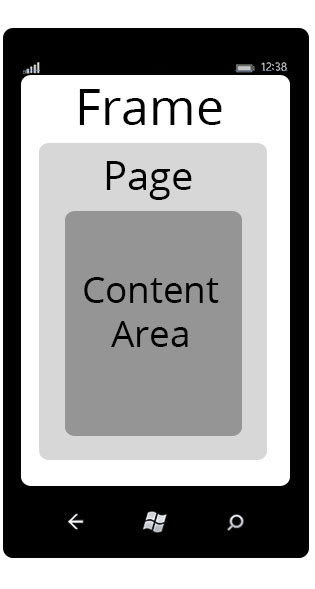
\includegraphics[scale=0.5]{Gambar/nav_hierarchy}
	\caption{Hirarki navigasi}
	\label{fig:nav_hierarchy}
\end{figure}


% SUBSUB Mengenai Tata Letak
\subsubsection{Kontrol Tata Letak}
\label{subsubsec:Kontrol Tata Letak}
\hspace{0.5cm} Kontrol tata letak merupakan penampung pada antarmuka Windows Phone untuk objek di antarmuka dan kontrol yang lain (tombol radio, \textit{textbox}, dan lain-lain). Kontrol tata letak digunakan untuk meletakan objek-objek di layar. Ketika pertama membuat aplikasi Windows Phone maka tata letak dasar sebagai penampung akan langsung dibuat berikut panel judul dan panel konten. Selanjutnya untuk penambahan kontrol tata letak yang lain dapat ditambahkan di panel konten.


\hspace{0.5cm} Terdapat 3 jenis panel yang digunakan untuk menangani tata Letak yaitu \textit{Grid}, \textit{StackPane}, dan \textit{Canvas}. Perlu diperhatikan bahwa setiap halaman hanya memiliki satu jenis panel. Berikut adalah 3 jenis panel pada Windows Phone:

\begin{itemize}
	\item \textit{StackPanel} merupakan panel yang memposisikan element menjadi 1 baris dan beberapa elemen di setiap halaman diposisikan horizontal atau vertical saja.
	\item \textit{Grid} merupakan panel yang mendukung tata letak yang rumit. Panel ini memposisikan elemen di baris dan kolom mana saja di setiap halaman.
	\item \textit{Canvas} memposiskan elemen sebagai absolut kordinat. Jadi setiap elemen di dalam \textit{canvas} dapat diposisikan spesifik sesuai kordinat x dan y.
\end{itemize}

Kode untuk mengatur jenis panel pada Windows Phone dapat dilihat pada \textit{listing}~\ref{lst:grid}.
\begin{lstlisting} [caption= {Kode tata letak grid},label={lst:grid}]
	<Grid x:Name="ContentPanel">
	</Grid>
\end{lstlisting}
	
% SUBSUB Mengenai Kontrol Masukan
\subsubsection{Kontrol Terhadap Teks}
\label{subsubsec:Kontrol Terhadap Teks}
\hspace{0.5cm} Kontrol terhadap teks  akan menampilkan konten yang memiliki tipe \textit{String}. Terdapat berbagai macam kontrol terhadap teks di Windows Phone yaitu \textit{TextBlock}, \textit{TextBox} dan \textit{PasswordBox}. Ketiga macam kontrol tersebut dibedakan berdasarkan tujuannya. Berikut keterangan, gambar~\ref{fig:kontrol_teks}, dan kode pada \textit{listing}~\ref{lst:text} kontrol teks.

\begin{itemize}
	\item \textit{TextBlock} merupakan tempat menaruh potongan teks yang hanya bisa dilihat.
	\item \textit{TextBox} biasanya digunakan untuk teks masukan yang pendek. Tapi bisa juga dipakai untuk masukan yang banyak dan beberapa baris.
	\item \textit{PasswordBox} biasanya digunakan untuk masukan yang bersifat rahasia. Karakter yang dimasukan langsung disamarkan menjadi bentuk titik.
\end{itemize}

\begin{figure}[h]
	\centering
		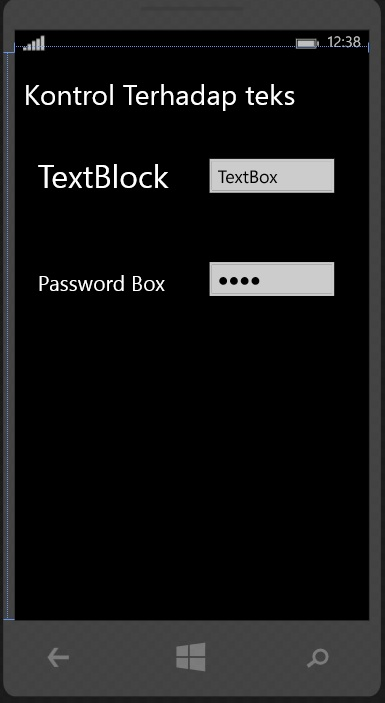
\includegraphics[scale=0.5]{Gambar/Tombol/kontrol_teks}
	\caption{\textit{TextBlock}, \textit{TextBox} dan \textit{PasswordBox}}
	\label{fig:kontrol_teks}
\end{figure}

\begin{lstlisting} [caption= {Kode untuk menampilkan \textit{TextBlock} dan \textit{TextBox}},label={lst:text}]
	<TextBlock x:Name="TextBlock1" Text="TextBlock"/>
	<TextBox x:Name="TextBox1"Text="TextBox"/>
\end{lstlisting}

% SUBSUB Mengenai Kontrol Masukan
\subsubsection{Tombol dan Kontrol Pilihan}
\label{subsubsec:Tombol dan Kontrol Pilihan}
\hspace{0.5cm} Tombol memungkinkan pengguna untuk berpindah halaman. Sedangkan kontrol pilihan memudahkan dalam memilih. Berikut keterangan, gambar~\ref{fig:kontrol_tombol}, dan kode pada \textit{listing}~\ref{lst:tombol} tombol dan kontrol pilihan.
 
\begin{itemize}
	\item \textit{Button} merupakan kontrol yang dipakai pengguna untuk mengaktifkan \textit{event} tekan.
	\item \textit{HyperlinkButton} merupakan kontrol yang menampilkan tautan. Jika \textit{HyperlinkButton} ditekan maka akan berpindah ke halaman yang akan dituju.	
	\item \textit{CheckBox} merupakan kontrol yang memungkinkan pengguna memilih beberapa item.
	\item \textit{RadioButton} merupakan kontrol yang memungkinkan pengguna memilih satu pilihan dari beberapa pilihan.
	\item \textit{Slider} merupakan kontrol yang memungkinkan pengguna memilih nilai kisaran dari jalur yang sudah disediakan.
\end{itemize}

\begin{figure}[h]
	\centering
		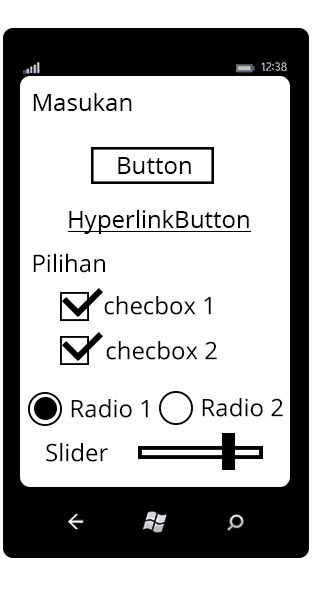
\includegraphics[scale=0.5]{Gambar/Tombol/tombol_dan_pilihan}
	\caption{Gambar kontrol pada Windows Phone}
	\label{fig:kontrol_tombol}
\end{figure}

\begin{lstlisting} [caption= {Kode untuk menampilkan \textit{TextBlock}, \textit{TextBox}, dan \textit{PasswordBox}},label={lst:tombol}]
	<Button x:Name="find" Content="Button"/>
\end{lstlisting}

% SUBSUB Kontrol Daftar
\subsubsection{Kontrol Daftar}
\label{subsubsec:Kontrol Daftar}
\hspace{0.5cm} Kontrol yang dipakai untuk menampilkan daftar dari beberapa \textit{item}. Berikut keterangan, gambar~\ref{fig:antarmukaListBox}, dan kode pada \textit{listing}~\ref{lst:listBox} kontrol daftar. 

\begin{itemize}
	\item \textit{ListBox} akan menampilkan daftar \textit{item}. Daftar ini dapat dipilih dengan cara ditekan.
	\item \textit{LongListSelector} dipakai untuk mengelompokan, menampilkan, dan melakukan penggulungan terhadap daftar yang panjang.
\end{itemize}

\begin{figure}[h]
	\centering
		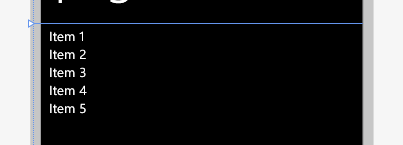
\includegraphics[scale=0.4]{Gambar/kontrol/listBox.PNG}
	\caption{Antarmuka \textit{ListBox}}
	\label{fig:antarmukaListBox}
\end{figure}

\begin{lstlisting} [caption= {Kode untuk menampilkan \textit{listBox}},label={lst:listBox}]
	<ListBox>
		<ListBoxItem Content="Item 1" />
		<ListBoxItem Content="Item 2" />
		<ListBoxItem Content="Item 3" />
		<ListBoxItem Content="Item 4" />
		<ListBoxItem Content="Item 5" />
	</ListBox>
\end{lstlisting}

% SUB Mengenai Siklus Hidup Aplikasi
\subsection{Siklus Hidup Aplikasi}
\label{subsec:Siklus Hidup Aplikasi}
\hspace{0.5cm} Siklus hidup aplikasi merupakan waktu mulai dari aplikasi dijalankan sampai dengan aplikasi diberhentikan dari memori. Siklus hidup aplikasi penting diketahui agar pengguna tidak kecewa menggunakan aplikasi serta memastikan sumber daya tersedia (dalam aplikasi ini yaitu sumber daya GPS). Seringkali pengguna tidak berhati-hati dalam menggunakan aplikasi, maka dari itu penulis harus memahami kapan aplikasi harus diaktifkan, ditangguhkan, atau bahkan dinonaktifkan karena sudah tidak digunakan. Gambar~\ref{fig:Siklus Hidup Aplikasi} adalah ilustrasi dari siklus hidup pada Windows Phone.

\begin{figure}[h]
	\centering
		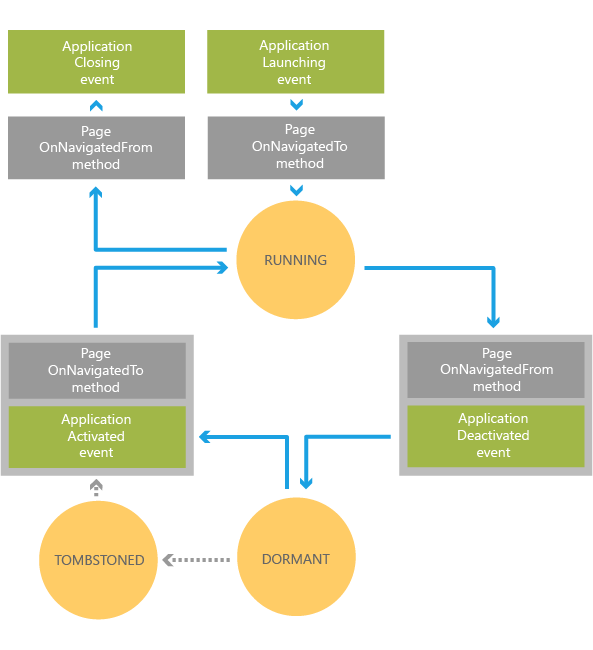
\includegraphics[scale=0.4]{Gambar/lifecycle_wp8}
	\caption{Gambar siklus hidup aplikasi\cite{MSDN}}
	\label{fig:Siklus Hidup Aplikasi}
\end{figure}
%sumber http://msdn.microsoft.com/en-us/library/windows/apps/ff817008%28v=vs.105%29.aspx

Sesuai gambar~\ref{fig:Siklus Hidup Aplikasi} lingkaran melambangkan keadaan aplikasi, persegi panjang menunjukan peristiwa aplikasi atau tingkat peristiwa di halaman. Berikut ini adalah keterangan untuk siklus hidup Windows Phone pada gambar~\ref{fig:Siklus Hidup Aplikasi}. 
\begin{itemize}
	\item \textit{The Launching Event} \\
	Merupakan tampilan awal saat aplikasi dipilih yang memberitahukan pengguna bahwa aplikasi sedang dijalankan. \textit{Event} ini akan dipanggil ketika aplikasi di jalankan pertama kali. \textit{Event} ini akan berjalan di belakang (\textit{background processing}) ketika aplikasi ditutup sementara atau sedang berada pada keadaan \textit{Dormant} atau \textit{Tombstoned} menjadi \textit{running}.
	\item \textit{Running} \\
	Setelah dijalankan, aplikasi akan masuk ke keadaan \textit{running}. Hal ini akan terus berlangsung sampai pengguna berpindah ke halaman depan, atau mundur melewati halaman utama aplikasi. Aplikasi keluar dari keadaan \textit{running} jika perangkat di kunci. Keadaan \textit{running} masih dapat terjadi saat perangkat di kunci dengan menonaktifkan \textit{idle detection} pada aplikasi.
	\item Metode \textit{OnNavigatedFrom} \\
	Merupakan metode yang dipanggil ketika berpindah ke halaman lain aplikasi. Ketika metode ini dipanggil maka aplikasi akan menyimpan keadaan dari halaman sebelum ditinggalkan. Hal tersebut dibutuhkan agar halaman tersebut bisa dikembalikan ke keadaan sebelum ditinggalkan saat pengguna ingin kembali ke halaman tersebut. Pemanggilan dilakukan ketika berpindah antara halaman di aplikasi atau ketika berpindah aplikasi.
	\item \textit{The Deactivated Event} \\
	\textit{Event} ini akan terjadi ketika pengguna berpindah aplikasi dan menekan tombol "\textit{start}" atau menjalankan aplikasi lain. Untuk penanganan \textit{deactivated event}, aplikasi harus menyimpan data sebelumnya, sehingga data sebelumnya dapat dikembalikan suatu saat. Windows Phone 8 juga mendukung sistem pengembalian data dengan \textit{State Object}. \textit{State Object} akan digunakan untuk menyimpan keadaan aplikasi sebelum aplikasi dinonaktifkan. 
	\item \textit{Dormant} \\
	Keadaan ini akan terjadi setelah \textit{deactivated event}. Pada keadaan ini, semua \textit{thread} aplikasi akan dihentikan dan tidak ada proses yang terjadi, tetapi kondisi aplikasi tetap utuh di memori. Tetapi jika sistem operasi membutuhkan memori yang lebih besar maka aplikasi yang dalam keadaan \textit{Dormant} akan menjadi \textit{Tombstone} untuk membebaskan memori.
	\item \textit{Tombstoned} \\
	Aplikasi yang masuk ke keadaan \textit{Tombstoned} akan dihentikan, namun sistem operasi akan menyimpan informasi aplikasi pada saat aplikasi berada di keadaan \textit{deactivated}.
	\item \textit{The Activated Event} \\
	\textit{Event} ini dipanggil ketika aplikasi meninggalkan keadaan \textit{Dormant} atau \textit{Tombstoned}. Operasi ini dilakukan pada latar belakang. 
	\item \textit{The OnNavigatedTo Method} \\
	Metode ini dipanggil ketika pengguna berpindah ke halaman yang sebelumya ditinggalkan. Metode ini akan memeriksa keadaan aplikasi dan memulihkannya jika keadaan sebelumnya pernah disimpan. 
	\item \textit{The Closing Event} \\
	\textit{Event} ini akan tercapai ketika pengguna berpindah mundur keluar dari halaman utama. Pada kasus ini, aplikasi akan dihentikan dan tidak ada keadaan yang disimpan. 
\end{itemize}

% SUB Peta di Windows Phone
\subsection{Peta di Windows Phone}
\label{subsec:Peta di Windows Phone}
\hspace{0.5cm} Peta yang dipakai di Windows Phone adalah \textit{Windows Phone Maps}. Windows Phone menawarkan beberapa pilihan dalam tampilan peta mulai dari kartografi, pencahayaan dan pandangan. Selain tampilan pada Sub Bab ini akan dibahas mengenai mendapatkan lokasi, petunjuk arah, \textit{MapPolyline} dan \textit{Pushpin}.

% SUBSUB Mengenai Penambahan Peta Ke Aplikasi
\subsubsection{Penambahan Peta Ke Aplikasi}
\label{subsubsec:Penambahan Peta Ke Aplikasi}
\hspace{0.5cm} Untuk penambahan peta pada Windows Phone menggunakan kontrol peta. Kontrol peta merupakan bagian dari \textit{library} Windows Phone. Dengan begitu untuk dapat menggunakannya perlu direferensikan. Untuk dapat menggunakannya juga harus ditambah \textit{capability} ID\_CAP\_MAP. Setelah hal tersebut dilakukan barulah peta dapat ditampilkan. Berikut gambar~\ref{fig:peta}, kode XAML pada \textit{listing}~\ref{lst:mapXAML}, dan kode program pada \textit{listing}~\ref{lst:mapCode} peta.

\begin{figure}[h]
	\centering
		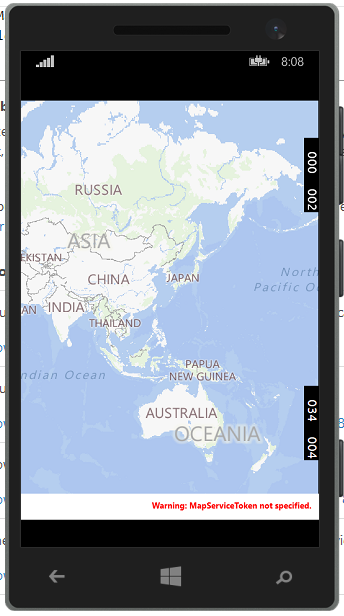
\includegraphics[scale=0.1]{Gambar/map}
	\caption{Tampilan peta pada Windows Phone}
	\label{fig:peta}
\end{figure}

\begin{lstlisting} [caption= {Menampilkan peta dengan nama MyMap dari XAML},label={lst:mapXAML}]
	<Controls:Map x:Name="MyMap"/>
\end{lstlisting}

\begin{lstlisting} [caption= {Menampilkan peta dengan nama MyMap dari kode program},label={lst:mapCode}]
	public mapFrom()
  {
		InitializeComponent();
		Map MyMap = new Map();
		ContentPanel.Children.Add(MyMap);
  }
\end{lstlisting}

% SUBSUB Tampilan Peta di Windows Phone
\subsubsection{Tampilan Peta di Windows Phone}
\label{subsubsec:Tampilan Peta di Windows Phone}
\hspace{0.5cm} Dalam tampilannya ada beberapa hal yang perlu diperhatikan agar pengguna merasa nyaman saat melihat peta di Windows Phone. Beberapa tampilan yang bisa ditampilkan dibuat untuk hal yang berbeda-beda. Berikut akan dibahas menentukan pusat dan tingkat zoom, kartografi, warna dan tampilan peta.

\begin{itemize}
	\item Menentukan pusat peta berarti menentukan titik tengah sebagai pandangan awal di peta. Untuk penentuan titik tengah dibutuhkan 2 nilai yaitu \textit{latitude} dan \textit{longitude}. Sedangkan \textit{zoom} merupakan properti untuk mengatur seberapa dekat atau jauh pandangan yang akan ditampilkan di peta. \textit{Zoom} memiliki nilai yang bisa diatur dari satu hingga dua puluh. Kode untuk mengatur titik tengah peta dan tingkat \textit{zoom} dapat dilihat pada \textit{listing}~\ref{lst:zoomXAML} dan \textit{listing}~\ref{lst:zoomCode}.\\
	
	\begin{lstlisting} [caption= {Mengatur tingkat zoom dari XAML},label={lst:zoomXAML}]
		<Controls:Map x:Name="MyMap" ZoomLevel="10" Margin="-25,0,-16,0"/>
	\end{lstlisting}

	\begin{lstlisting} [caption= {Mengatur tingkat zoom dari dari kode program},label={lst:zoomCode}]
		public mapFrom()
		{
			InitializeComponent();
			Map MyMap = new Map();

			//Mengatur titik tengah peta
			MyMap.Center = new GeoCoordinate(47.6097, -122.3331);

			//mengatur tingkat zoom
			MyMap.ZoomLevel = 10;
			ContentPanel.Children.Add(MyMap);
		}
	\end{lstlisting}

	
	\item Kartografi peta di Windows Phone merupakan cara pandang dalam melihat dan menerjemahkan peta. Terdapat empat jenis kartografi, yaitu:
		
		\begin{itemize}
			\item \textit{Road}: Tampilan normal 2 dimensi.
			\item \textit{Aerial}: Tampilan peta yang diambil dari foto di udara.
			\item \textit{Hybrid}: Tampilan Aerial yang digabung dengan jalan dan label.
			\item \textit{Terrain}: Menampilkan gambar fisik bumi termasuk ketinggian dan air.
		\end{itemize}
		
		\begin{figure}[h]
			\centering
				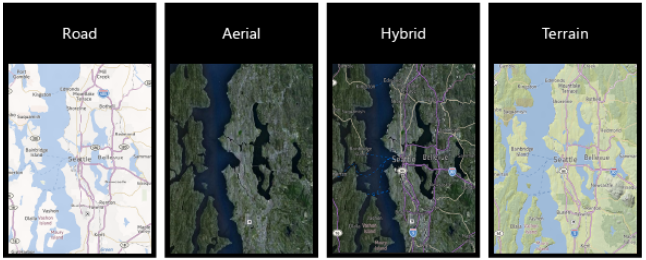
\includegraphics[scale=0.4]{Gambar/kartografi}
			\caption{Kartografi}
			\label{fig:Kartografi}
		\end{figure}
		
	\item	Mode warna yang disediakan Windows Phone ada dua yaitu terang dan gelap. Secara \textit{default} mode pada peta di Windows Phone adalah terang.
	
	\item Tampilan pada Peta di Windows Phone dapat berubah karena hasil diputar, dimiringkan, ditarik, dan diturunkan. Berikut beberapa hal yang dapat diatur sebagai tampilan di peta.
	
		\begin{itemize}
			\item \textit{Heading} merupakan representasi dari derajat secara geometri. Derajat ini didefinisikan dalam 0 sampai 360 yang dipakai untuk memutar peta. Contoh, 0 atau 360 ke arah utara, 90 ke arah barat, 180 ke arah selatan, dan 270 derajat ke arah timur.
			\item \textit{Pitch} merupakan derajat kemiringan dari peta dari sudut pengguna. Contoh, \textit{Pitch} = 0 berarti melihat dari atas ke bawah sedangkan \textit{Pitch} = 45 berarti melihat dari samping ke bawah dengan sudut 45 derajat.
		\end{itemize} 
\end{itemize}

% SUBSUB Pushpin ke Peta
\subsubsection{\textit{Pushpin} ke Peta}
\label{subsubsec:Pushpin ke Peta}
\hspace{0.5cm} \textit{Pushpin} merupakan elemen yang dapat ditempatkan pada peta secara spesifik dan bisa dipakai untuk interaksi pada peta. Peta tidak mendukung langsung penggunaan \textit{pushpin} karena merupakan elemen dari \textit{MapOverlay} (bagian/lapisan terpisah dari peta). Untungnya di Windows Phone memiliki Windows Phone 8 \textit{Toolkit} yang memiliki set objek agar dapat menggunakan \textit{pushpin} pada peta di Windows Phone. Contoh keluaran \textit{pushpin} dapat dilihat pada Gambar~\ref{fig:toolkit_pushpin} dan kode untuk menampilkannya dapat dilihat pada \textit{listing}~\ref{lst:pushpin}.

\begin{figure}[h]
	\centering
		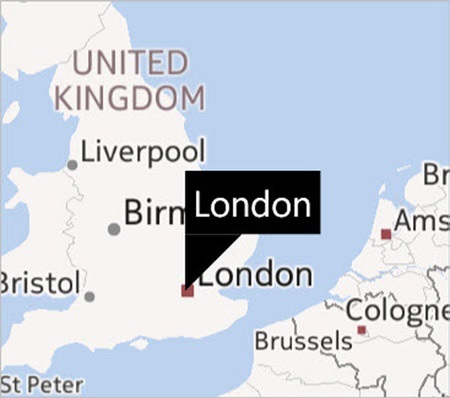
\includegraphics[scale=0.5]{Gambar/toolkit_pushpin}
	\caption{Keluaran Toolkit Pushpin pada peta \cite{Manning}}
	\label{fig:toolkit_pushpin}
\end{figure}

\begin{lstlisting} [caption= {Kode untuk menampilkan pushpin},label={lst:pushpin}]
	MapOverlay overlay = new MapOverlay
	{
		GeoCoordinate = map.Center,
		Content = new Border
		{
		BorderBrush = new SolidColorBrush(Color.FromArgb(120, 255, 0, 0)),
		Child = new TextBlock(){Text="Pushpin"},
		BorderThickness = new Thickness(1),
		Background = new SolidColorBrush(Color.FromArgb(120,255,0,0)),
		Width = 80,
		Height = 60
		}
	};
	MapLayer layer = new MapLayer();
	layer.Add(overlay);

	map.Layers.Add(layer);
\end{lstlisting}

% SUBSUB Polyline pada Peta
\subsubsection{\textit{Polyline} pada Peta}
\label{subsubsec:Polyline pada Peta}
\hspace{0.5cm} Dalam menentukan arah dibutuhkan dua titik yaitu titk awal dan titik tujuan. Tentu saja arah tersebut butuh ditandai dengan garis. \textit{Polyline} merupakan tentetan garis lurus yang saling terhubung satu sama lain. Dengan \textit{polyline} arah pada peta dapat ditandai dengan warna maupin tebal atau tipisnya garis. Contoh keluaran \textit{polyline} dapat dilihat pada Gambar~\ref{fig:TampilanpolylinepadaPeta} dan kode untuk menampilkannya dapat dilihat pada \textit{listing}~\ref{lst:polyline}.

\begin{figure}[h]
	\centering
		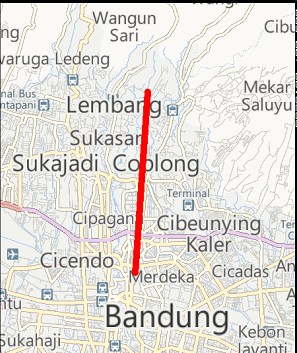
\includegraphics[scale=0.5]{Gambar/kontrol/polyline}
	\caption{Tampilan polyline pada Peta}
	\label{fig:TampilanpolylinepadaPeta}
\end{figure}

\begin{lstlisting} [caption= {Kode untuk menampilkan polyline},label={lst:polyline}]
	MapPolyline line = new MapPolyline();
	line.StrokeColor = Colors.Red;
	line.StrokeThickness = 10;
	line.Path.Add(new GeoCoordinate(-6.8619546, 107.614441));
	line.Path.Add(new GeoCoordinate(-6.908693, 107.611185));
\end{lstlisting}

% SUBSUB Namespace Map
\subsubsection{\textit{Namespace Control Map}}
\label{subsubsec:Namespace Control Map}
\hspace{0.5cm} \textit{Namespace} merupakan nama yang dipakai untuk mengatur kelas-kelas. Windows Phone 8 sudah menyediakan \textit{namespace} bawaan untuk mengatur peta. \textit{Namespace} yang disediakan adalah \textit{Maps.Controls}. \textit{Namespace} ini yang berisi kelas-kelas yang paling sering digunakan untuk mengatur peta pada Windows Phone.  Agar dapat menggunakan kelas pada \textit{namespace} tersebut perlu ditambahkan \textit{namespace} dan \textit{capabilities}. \textit{Namespace} yang harus ditambahkan pada baris awal XAML adalah \textit{Microsoft.Phone.Maps.Controls}. Selanjutnya ada penambahan \textit{capabilities} \textit{ID\_CAP\_MAP}. Penambahan \textit{capabilities} ditambahkan pada \textit{WMAppManifest.xml}.

% SUBSUB Kelas Map
\subsubsection{Kelas Map}
\label{subsubsec:Kelas Map}
\hspace{0.5cm} Merupakan kelas yang mewakili kontrol map.

Berikut properti yang dapat digunakan pada kelas ini.
\begin{table}[h]
	\centering
		\begin{tabular}{ |c|c|}
				\hline
					Nama & Deskripsi \\ \hline
					\textit{CartographicMode} & Mengatur dan mendapatkan tipe dari peta. \\ \hline
					\textit{Center} & Mengatur dan mendapatkan titik tengah pada peta. \\ \hline
					\textit{ColorMode} & Mengatur dan mendapatkan mode warna peta. \\ \hline
					\textit{Heading} & Mengatur dan mendapatkan arah pandang peta. \\ \hline
					\textit{Height} & Mengatur dan mendapatkan tinggi. \\ \hline
					\textit{LandmarksEnabled} & Indikasi apakah bangunan 3D ditampilkan. \\ \hline
					\textit{Name} & Mengatur dan mendapatkan nama untuk identifikasi objek. \\ \hline
					\textit{PedestrianFeaturesEnabled} & Indikasi fitur pejalan kaki ditampilkan. \\ \hline
					\textit{Pitch} & Mengatur dan mendapatkan derajat kemiringan peta. \\ \hline
					\textit{Tag} & Mengatur dan mendapatkan nilai objek. \\ \hline
					\textit{TileSources} & Mendapatkan koleksi lapisan lantai. \\ \hline
					\textit{Width} & Mengatur dan mendapatkan lebar. \\ \hline
					\textit{ZoomLevel} & Mengatur dan mendapatkan tingkat zoom pada peta. \\ \hline
				\hline
		\end{tabular}
	\caption{Properti kelas Map}
	\label{tab:PropertiKelasMap}
\end{table}

Berikut metode yang dapat digunakan pada kelas ini.
\begin{itemize}
	\item \textit{SetView(LocationRectangle)} \\
	Metode untuk mengatur pandangan di atas peta secara spesifik sesuai wilayah geografis. Metode ini tidak mengembalikan nilai.
	\item \textit{SetView(GeoCoordinate, Double)} \\
	Metode untuk mengatur pandangan di atas peta secara spesifik sesuai titik tengah dan tingkat zoom. Metode ini tidak mengembalikan nilai.
	\item \textit{SetView(LocationRectangle, MapAnimationKind)}\\
	Metode untuk mengatur pandangan di atas peta secara spesifik sesuai region geografis dan animasi. Metode ini tidak mengembalikan nilai.
	\item \textit{SetView(LocationRectangle, Thickness)} \\
	Metode untuk mengatur pandangan di atas peta secara spesifik sesuai region geografis dengan batas tertentu. Metode ini tidak mengembalikan nilai.
	\item \textit{SetView(GeoCoordinate, Double, MapAnimationKind)} \\
	Metode untuk mengatur pandangan di atas peta secara spesifik sesuai titik tengah, tingkat zoom, dan animasi. Metode ini tidak mengambalikan nilai.
	\item \textit{SetView(GeoCoordinate, Double, Double)} \\
	Metode untuk mengatur pandangan di atas peta secara spesifik sesuai titik tengah, tingkat zoom, dan \textit{heading}. Metode ini tidak mengembalikan nilai.
	\item \textit{SetView(LocationRectangle, Thickness, MapAnimationKind)} \\
	Metode untuk mengatur pandangan di atas peta secara spesifik sesuai wilayah geografis dengan batas tertentu, dan animasi. Metode ini tidak mengembalikan nilai.
	\item \textit{SetView(GeoCoordinate, Double, Double, MapAnimationKind)} \\
	Metode untuk mengatur pandangan di atas peta secara spesifik sesuai titik tengah, tingkat zoom, \textit{heading}, dan animasi. Metode ini tidak mengembalikan nilai.	
	\item \textit{SetView(GeoCoordinate, Double, Double, Double)} \\
	Metode untuk mengatur pandangan di atas peta secara spesifik sesuai titik tengah, tingkat zoom, \textit{heading}, \textit{pitch}. Metode ini tidak mengembalikan nilai.
	\item \textit{SetView(GeoCoordinate, Double, Double, Double, MapAnimationKind)} \\
	Metode untuk mengatur pandangan di atas peta secara spesifik sesuai titik tengah, tingkat zoom, \textit{heading}, \textit{pitch}, dan animasi. Metode ini tidak mengembalikan nilai.
	\item \textit{UpdateLayout} \\
	Metode yang memastikan semua posisi objek turunan mengikuti tata letak. 
\end{itemize}

% SUBSUB Polyline Class
\subsubsection{\textit{Polyline Class}}
\label{subsubsec:Polyline Class}
\hspace{0.5cm} Merupakan kelas yang dipakai untuk menggambarkan garis lurus yang saling terhubung. Kelas ini tergabung ke dalam \textit{namespace Microsoft.Phone.Maps.Controls}. 

Berikut properti yang dapat digunakan pada kelas ini.
\begin{table}[h]
	\centering
		\begin{tabular}{ |c|c|}
				\hline
					Nama & Deskripsi \\ \hline
					\textit{Dispacher} & Mendapatkan objek yang terkait. \\ \hline
					\textit{Path} & Mengatur dan mendapatkan kumpulan nilai \textit{GeoCoordinates} yang membuat \textit{polyline}. \\ \hline
					\textit{StrokeColor} & Mengatur dan mendapatkan warna garis. \\ \hline
					\textit{StrokeDashed} & Mengatur dan mendapatkan nilai untuk menggambar \textit{polyline} pustus-putus. \\ \hline
					\textit{StrokeThickness} & Mengatur dan mendapatkan lebar garis untuk menggambar \textit{polyline}. \\ \hline
				\hline
		\end{tabular}
	\caption{Properti \textit{Polyline Class}}
	\label{tab:PropertiKelasPolyline}
\end{table}

Berikut metode yang dapat digunakan pada kelas ini.
\begin{itemize}
	\item \textit{CheckAccess}\\
	Metode yang menentukan bisa atau tidaknya pemanggilan \textit{thread} untuk mengakses objek.
	\item \textit{ClearValue}\\
	Metode yang akan membersihkan nilai lokal
	\item \textit{Finalize} \\
	Metode yang dipakai untuk melakukan pembersihan pada sumber daya yang tidak terpakai sebelum objek dihancurkan.
\end{itemize}

% SUBSUB Pushpin Class
\subsubsection{\textit{Pushpin Class}}
\label{subsubsec:Pushpin Class}
\hspace{0.5cm} Merupakan kelas yang dipakai untuk menggambarkan elemen terpisah diatas peta. Meskipun pushpin merupakan bawaan pada peta untuk menunjuk suatu lokasi tetapi \textit{pushpin} dari peta tidak dapat diubah-ubah. \textit{Pushpin} pada Windows Phone 8 dapat dibuat sesuai kebutuhan. Namun ada cara lain dengan menambahkan Windows Phone Toolkit. Windows Phone Toolkit mempunyai komponan untuk menggambar pushpin diatas peta.  
%sumber http://developer.nokia.com/resources/library/Lumia/change-history/archived-content/maps-and-navigation/guide-to-the-wp8-maps-api.html

% SUB Lokasi
\subsection{Lokasi}
\label{subsec:Lokasi}
\hspace{0.5cm} Aplikasi di Windows Phone 8 dapat memanfaatkan lokasi dimana perangkat berada. Aplikasi dapat melacak lokasi sesaat  pengguna atau pelacakan selama periode tertentu. Data lokasi perangkat berasal dari berbagai sumber termasuk \textit{Global Positioning System} (GPS), \textit{Wireless Fidelity} (Wi-Fi), dan jaringan seluler. Ada 2 set API berbeda yang dapat dimanfaatkan di Windows Phone yaitu \textit{Runtime Location} API dan .NET \textit{Location} API. Windows Phone \textit{Runtime Location} memiliki keunggulan fitur yang banyak sedangkan .NET \textit{Location} direkomendasikan jika aplikasi ditargetkan pada Windows Phone 7.1 dan Windows Phone 8.

\hspace{0.5cm} Hal yang perlu diperhatikan dalam menentukan layanan lokasi adalah penangkap GPS, Wi-Fi, dan jaringan seluler. Perangkat tersebut berfungsi sebagai penyedia data lokasi dengan berbagai tingkat akurasi dan konsumsi daya. Perangkat diatas juga berkomunikasi langsung untuk memutuskan sumber mana yang digunakan untuk menentukan lokasi perangkat berdasarkan ketersediaan data lokasi dan prasyarat yang ditentukan aplikasi. Lapisan diatas penyedia data lokasi tersebut adalah pengelola antarmuka. Aplikasi akan mengunakan antarmuka tersebut untuk memulai dan menghentikan layanan lokasi, mengatur tingkat akurasi, dan menerima data lokasi.

\hspace{0.5cm} Karena pengguna dapat berpindah tempat untuk menuju tempat yang lain, maka pelacakan lokasi harus dilakukan terus menerus. Pelacakan lokasi secara terus menerus ini dapat dilakukan di depan maupun di belakang aplikasi Windows Phone 8. Pelacakan aplikasi di depan akan memungkinkan aplikasi melacak lokasi pengguna sekaligus melakukan perbaruan antarmuka. Jika pelacakan lokasi di belakang aplikasi maka tidak ada perubahan pada antarmuka namun pelacakan dilakuan secara terus menerus. Pelacakan yang terus menerus di belakang aplikasi akan membuat keadaan aplikasi cepat dipulihkan dari keadaan \textit{Dormant}.

% SUBSUB Mendapatkan Posisi Pengguna
\subsubsection{Mendapatkan Posisi Pengguna}
\label{subsubsec:Mendapatkan Posisi Pengguna}
\hspace{0.5cm} Di Windows Phone 8 telah ada \textit{GeoCoordinate class} yang dapat digunakan untuk mengetahui posisi pengguna. \textit{Geolocator class} dari \textit{Windows.Devices.Geolocation} akan mengembalikan posisi saat ini. Untuk menggunakan \textit{Geolocator}, perlu menghidupkan \textit{ID\_CAP\_LOCATION} di \textit{\textbackslash properties\textbackslash WMAppManifest.xml}. Dalam mendapatkan posisi perlu diperhatikan status dari GPS karena membutuhkan waktu dari awal pengaktifan hingga mendapatkan lokasi pengguna secara akurat. Untuk lebih jelas mengenai status posisi dapat dilihat pada nilai status dibawah ini.

\begin{itemize}
	\item \textit{Ready} : Jika lokasi tersedia.
	\item \textit{Initializing} : Jika status penangkap GPS belum memiliki cukup satelit untuk mendapatkan posisi yang akurat. 
	\item \textit{NoData} : Data lokasi belum tersedia. Status ini muncul jika aplikasi sedang mamanggil \textit{GetGeopositionAsync()} atau \textit{register}.
	\item \textit{Disable} : Status mengindikasikan tidak diperbolehkannya pengaksesan lokasi.
	\item \textit{NotInitialized} : Data lokasi belum tersedia. Status ini muncul jika aplikasi belum mamanggil \textit{GetGeopositionAsync()} atau \textit{register}.
	\item \textit{NotAvailable} : Jika sensor arah mata angin dan lokasi tidak tersedia.
\end{itemize}

% SUBSUB Namespace Geolocator
\subsubsection{\textit{Namespace Geolocator}}
\label{subsubsec:Namespace Geolocator}
\hspace{0.5cm} \textit{Namespace} merupakan nama yang dipakai untuk mengatur kelas-kelas. Windows Phone 8 sudah menyediakan \textit{namespace} bawaan untuk mengakses lokasi. \textit{Namespace} yang disediakan adalah \textit{namespace geolocator}. \textit{Namespace} ini akan mengakses lokasi geografis dari perangkat dan mendukung pelacakan lokasi dari waktu ke waktu. Agar dapat menggunakan kelas pada \textit{namespace} tersebut perlu ditambahkan \textit{namespace} dan \textit{capabilities}. \textit{Namespace} yang harus ditambahkan pada baris awal XAML adalah \textbf{Windows.Device.Geolocator}. Selanjutnya ada penambahan \textit{capabilities ID\_CAP\_LOCATION}. Penambahan \textit{capabilities} ditambahkan pada \textit{WMAppManifest.xml}. Kelas yang diatur oleh \textit{namespace geolocator} dapat di lihat pada tabel ~\ref{tab:KelasPadaNamespaceGeolocator}.
\begin{table}[h]
	\centering
		\begin{tabular}{ |c|c|}
				\hline
				Kelas & Deskripsi \\ \hline
				\textit{Geocoordinate} & Berisi informasi untuk mengidentifikasi lokasi geografis. \\ \hline
				\textit{Geolocator} & Mendukung dalam pengaksesan lokasi perangkat. \\ \hline
				\textit{Geoposition} & Memberikan data lokasi beserta \textit{latitude} dan \textit{longitude} atau data alamat. \\ \hline
				\hline
		\end{tabular}
	\caption{Kelas pada \textit{Namespace Geolocator}}
	\label{tab:KelasPadaNamespaceGeolocator}
\end{table}

% SUBSUB Kelas Geocoordinate
\subsubsection{\textit{Geocoordinate}}
\label{subsubsec:Kelas Geocoordinate}
\hspace{0.5cm} Geocoordinate adalah kelas yang menunjukan lokasi sebagai kordinat geografis. Kelas ini hanya menyediakan properti yang hanya bisa dibaca. Kelas ini menyediakan properti yang ditunjukan pada tabel ~\ref{tab:PropertiPadaKelasGeocoordinate}.

\begin{table}[h]
	\centering
		\begin{tabular}{ |c|c|}
				\hline
				Properti & Deskripsi \\ \hline
				\textit{Altitude} & Ketinggian lokasi dalam satuan meter. \\ \hline
				\textit{Heading} & \vtop{\hbox{\strut Arah menghadap perangkat dalam satuan derajat yang} \hbox{\strut relative terhadap mata angin utara.}} \\ \hline
				\textit{Latitude} & Garis lintang dalam satuan derajat. \\ \hline
				\textit{Longitude}  & Garis bujur dalam satuan derajat. \\ \hline
				\textit{Point} & Lokasi dari \textit{Geocoordinate}. \\ \hline
				\textit{Speed} & Kecepatan dalam satuan meter per detik. \\ \hline
				\hline
		\end{tabular}
	\caption{Properti pada \textit{Geocoordinate}}
	\label{tab:PropertiPadaKelasGeocoordinate}
\end{table} 

% SUBSUB Kelas Geolocator
\subsubsection{\textit{Geolocator}}
\label{subsubsec:Kelas Geolocator}
\hspace{0.5cm} \textit{Geolocator} merupakan kelas yang mendukung pengaksesan terhadap lokasi.

Berikut metode yang disediakan \textit{Geolocator}:
\begin{itemize}
	\item \textit{public IAsyncOperation<Geoposition> GetGeopositionAsync()} \\
		Operator await diatas dimaksudkan untuk meminta posisi lokasi terus menerus sampai selesai dan menunda tugas yang lain. \\
		\textit{GetGeopositionAsync()} merupakan bawaan kelas \textit{Geolocator} akan meminta data lokasi dan menanganinya sampai selesai.
		Kembalian dari \textit{GetGeopositionAsync()} adalah objek \textit{Geoposition}.
\end{itemize}

Berikut Properti yang disediakan kelas Geolocator:
\begin{itemize}
	\item \textit{public PositionStatus LocationStatus { get; }} \\
		Merupakan properti dari kelas \textit{geolocator} untuk mendapatkan status posisi dengan mengembalikan kelas \textit{PositionStatus}. Status pada kelas \textit{PositionStatus} adalah \textit{Ready}, \textit{Initializing}, \textit{NoData}, \textit{Disable}, \textit{NotInitialized}, dan \textit{NotAvailable}.
	\item \textit{public PositionAccuracy DesiredAccuracy { get; set; }} \\
		Properti yang digunakan untuk mengatur dan mendapatkan tingkat akurasi. Untuk tingkat akurasi dapat dipilih tingkat \textit{High} untuk tingkat akurasi tinggi dan dipilih tingkat {Default} untuk menghemat daya. Keluaran dari properti ini adalah tipe data \textit{PositionAccuracy}.
	\item \textit{public Nullable<uint> DesiredAccuracyInMeters { get; set; }}\\
		Sama seperti properti \textit{DesiredAccuracy} diatas tetapi dalam satuan meter. Keluaran dari properti ini adalah tipe data \textit{uint}.
	\item \textit{public uint ReportInterval { get; set; }} \\
		Merupakan properti untuk mendapatkan selang waktu pembaruan lokasi. Properti ini mengeluarkan tipe data unit.
\end{itemize}

% SUBSUB Kelas Geoposition
\subsubsection{\textit{Geoposition}}
\label{subsubsec:Kelas Geoposition}
\hspace{0.5cm} \textit{Geoposition} merupakan kelas yang memuat lokasi (\textit{latitude} dan \textit{longitude}).
Berikut Properti yang disediakan kelas \textit{Geoposition}:
\begin{itemize}
	\item \textit{public CivicAddress CivicAddress { get; }} \\
		Data alamat sipil yang terkait dengan lokasi geografis.
	\item \textit{public Geocoordinate Coordinate { get; }} \\
		Data latitude dan longitude yang terkait lokasi geografis.
\end{itemize}

% SUB Memanfaatkan Sumber Data
\subsection{Memanfaatkan Sumber Data}
\label{subsec:Memanfaatkan Sumber Data}
\hspace{0.5cm} Hal yang penting dari sebuah aplikasi adalah informasi. Windows Phone 8 memiliki kemampuan dalam menghubungkan aplikasi dengan sumber data lainnya. Memanfaatkan sumber data ada dua cara yaitu yang lokal atau berada di perangkat dan \textit{web service}. \textit{Web Service} merupakan metode komunikasi antara dua perangkat melalui jaringan. 

\hspace{0.5cm} Sebelum data dapat dikirim antar perangkat perlu dilakukan \textit{Serialization}. \textit{Serialization} disini merupakan proses mentransformasikan objek ke format yang bisa dengan mudah dikirim melewati jaringan atau disimpan di database. Formatnya disini berupa string yang direpresentasikan sebagai objek di XML atau JSON(Javascript Object Notation). Ada beberapa objek yang dapat melakukan serialisasi, tetapi yang akan dibahas penulis disini hanya serialisasi JSON. 

\hspace{0.5cm} Banyak \textit{web service} yang mengembalikan data dalam format JSON. JSON memiliki struktur yang mudah dipahami dimana kurung kurawal mengindikasikan objek, kurung siku berarti array, dan properti berupa nama dan nilai pasangan yang dipisahkan oleh titik dua. JSON format memiliki ukuran data yang kecil dan baik untuk penggunaan perangkat bergerak. Untuk contoh format JSON dapat dilihat di bagian Kiri API pada Bab dua ini karena Kiri API menggunakan format JSON. Serialisasi menggunakan \textit{DataContractJsonSerializer} membuat serialisasi mudah untuk menerjemahkan form String JSON ke objek yang dapat langsung digunakan. \textit{DataContractJsonSerializer} memakai \textit{WriteObject()} untuk serialisasi and \textit{ReadObject()} untuk de-serialisasi.

% SUBSUB Kelas HttpClient
\subsubsection{\textit{HttpClient}}
\label{subsubsec:Kelas HttpClient}
\hspace{0.5cm} Merupakan Kelas yang dipakai untuk mengirim permintaan HTTP dan menerima kembalian HTTP dari \textit{Uniform Resource Identifier}(URI) yang dapat diidentifikasi. Berikut metode yang disediakan kelas \textit{HttpClient}.
\begin{itemize}
	\item \textit{DeleteAsync(Uri)} \\
	Metode yang dipakai untuk mengirimkan permintaan DELETE ke URI yang spesifik sebagai operasi \textit{asynchronous}. Maksud dari operasi \textit{asynchronous} adalah memungkinkan aplikasi untuk melanjutkan pekerjaan selagi metode ini dipanggil\footnotemark[2]. Metode ini membutuhkan parameter URI sebagai tujuan dari permintaan. Sedangkan kembaliannya berupa objek yang mewakili operasi \textit{asynchronous} disertai kemajuan. Objek tersebut memiliki 2 parameter yaitu hasil berupa pesan kembalian dari http dan kemajuan dari data yang dikirim.
	\item \textit{GetAsync(Uri)} \\
	Metode yang dipakai untuk mengirimkan permintaan \textit{GET} ke URI yang spesifik sebagai operasi \textit{asynchronous}. Maksud dari operasi \textit{asynchronous} adalah memungkinkan aplikasi untuk melanjutkan pekerjaan selagi metode ini dipanggil\footnotemark[2]. Metode ini membutuhkan parameter URI sebagai tujuan dari permintaan. Sedangkan kembaliannya berupa objek yang mewakili operasi \textit{asynchronous} disertai kemajuan. Objek tersebut memiliki 2 parameter yaitu hasil berupa pesan kembalian dari http dan kemajuan dari data yang dikirim.
	\item \textit{GetAsync(Uri,HttpCompletionOption)} \\
	Metode yang dipakai untuk mengirimkan permintaan \textit{GET} ke URI yang spesifik sebagai operasi \textit{asynchronous}. Maksud dari operasi \textit{asynchronous} adalah memungkinkan aplikasi untuk melanjutkan pekerjaan selagi metode ini dipanggil\footnotemark[2]. Metode ini membutuhkan parameter URI sebagai tujuan dari permintaan dan nilai tambahan yang dimaksukan sebagai indikasi operasi dianggap selesai. Sedangkan kembaliannya berupa objek yang mewakili operasi \textit{asynchronous} disertai kemajuan. Objek tersebut memiliki 2 parameter yaitu hasil berupa pesan kembalian dari http dan kemajuan dari data yang dikirim.
	\item \textit{GetBufferAsync(Uri)} \\
	Metode yang dipakai untuk mengirimkan permintaan \textit{GET} ke URI yang spesifik sebagai operasi \textit{asynchronous}. Maksud dari operasi \textit{asynchronous} adalah memungkinkan aplikasi untuk melanjutkan pekerjaan selagi metode ini dipanggil\footnotemark[2]. Metode ini membutuhkan parameter URI sebagai tujuan dari permintaan. Sedangkan kembaliannya berupa objek yang mewakili operasi \textit{asynchronous} disertai kemajuan. Objek tersebut memiliki 2 parameter yaitu hasil berupa pesan kembalian yang dikirimkan secara buffer(disimpan dalam memori) dan kemajuan dari data yang dikirim.
	\item \textit{GetInputStreamAsync(Uri)} \\
	Metode yang dipakai untuk mengirimkan permintaan \textit{GET} ke URI yang spesifik sebagai operasi \textit{asynchronous}. Maksud dari operasi \textit{asynchronous} adalah memungkinkan aplikasi untuk melanjutkan pekerjaan selagi metode ini dipanggil\footnotemark[2]. Metode ini membutuhkan parameter URI sebagai tujuan dari permintaan. Sedangkan kembaliannya berupa objek yang mewakili operasi \textit{asynchronous} disertai kemajuan. Objek tersebut memiliki 2 parameter yaitu hasil berupa pesan kembalian yang dikirimkan secara stream(langsung sesuai waktu) dan kemajuan dari data yang dikirim.
	\item \textit{GetStringAsync(Uri)} \\
	Metode yang dipakai untuk mengirimkan permintaan \textit{GET} ke URI yang spesifik sebagai operasi \textit{asynchronous}. Maksud dari operasi \textit{asynchronous} adalah memungkinkan aplikasi untuk melanjutkan pekerjaan selagi metode ini dipanggil\footnotemark[2]. Metode ini membutuhkan parameter URI sebagai tujuan dari permintaan. Sedangkan kembaliannya berupa objek yang mewakili operasi \textit{asynchronous} disertai kemajuan. Objek tersebut memiliki 2 parameter yaitu hasil berupa pesan kembalian dalam bentuk string dan kemajuan dari data yang dikirim.
	\item \textit{PostAsync(Uri)} \\
	Metode yang dipakai untuk mengirimkan permintaan \textit{POST} ke URI yang spesifik sebagai operasi \textit{asynchronous}. Maksud dari operasi \textit{asynchronous} adalah memungkinkan aplikasi untuk melanjutkan pekerjaan selagi metode ini dipanggil\footnotemark[2]. Metode ini membutuhkan parameter URI sebagai tujuan dari permintaan. Sedangkan kembaliannya berupa objek yang mewakili operasi \textit{asynchronous} disertai kemajuan. Objek tersebut memiliki 2 parameter yaitu hasil berupa pesan kembalian dari http dan kemajuan dari data yang dikirim.
	\item \textit{SendRequestAsync(HttpRequestMessage)} \\
	Metode yang dipakai untuk mengirimkan permintaan HTTP sebagai operasi \textit{asynchronous}. Maksud dari operasi \textit{asynchronous} adalah memungkinkan aplikasi untuk melanjutkan pekerjaan selagi metode ini dipanggil\footnotemark[2]. Metode ini membutuhkan parameter pesan dari permintaan. Sedangkan kembaliannya berupa objek yang mewakili operasi \textit{asynchronous} disertai kemajuan. Objek tersebut memiliki 2 parameter yaitu hasil berupa pesan kembalian dari http dan kemajuan dari data yang dikirim.
	\item \textit{SendRequestAsync(HttpRequestMessage, HttpCompletionOption)} \\
	Metode yang dipakai untuk mengirimkan permintaan HTTP sebagai operasi \textit{asynchronous}. Maksud dari operasi \textit{asynchronous} adalah memungkinkan aplikasi untuk melanjutkan pekerjaan selagi metode ini dipanggil\footnotemark[2]. Metode ini membutuhkan parameter pesan dari permintaan dan nilai tambahan yang dimaksukan sebagai indikasi operasi dianggap selesai. Sedangkan kembaliannya berupa objek yang mewakili operasi \textit{asynchronous} disertai kemajuan. Objek tersebut memiliki 2 parameter yaitu hasil berupa pesan kembalian dari http dan kemajuan dari data yang dikirim.
\end{itemize}

\footnotetext[2]{\url{http://msdn.microsoft.com/en-us/library/ms734701\%28v=vs.110\%29.aspx}}
% http://msdn.microsoft.com/en-us/library/windows/apps/xaml/dn440594.aspx
% http://msdn.microsoft.com/en-us/library/windows/apps/xaml/windows.web.http.httpclient.aspx

% Kiri API
\section{Kiri API}
\label{sec:Kiri API}
\hspace{0.5cm} API atau \textit{Application Programming Interface} merupakan aturan yang dikodekan secara spesifik yang dapat digunakan untuk komunikasi antar aplikasi. Jadi API disini memfasilitasi untuk pemanggilan fungsi-fungsi tertentu diluar aplikasi itu sendiri. Pemanfaatan Kiri API dilakukan dengan menggunakan JSON atau \textit{JavaScript Object Notation} format. 

\hspace{0.5cm} Pemanfaatan Kiri API dengan melakuan permintaan dengan parameter \textit{POST} atau \textit{GET} lalu Kiri akan mengembalikan hasil dalam format JSON. Permintaan tersebut dikirimkan ke URL atau \textit{Uniform Resource Locator}. Berikut URL yang disediakan Kiri Api.
\begin{itemize}
	\item \url{http://preview.kiri.travel/handle.php} \\
	Merupakan URL untuk uji coba. Untuk kemampuannya juga menurut dokumentasi Kiri API masih tidak stabil.
	\item \url{http://kiri.travel/handle.php} \\
	Merupakan URL produksi. Ini merupakan URL yang direkomendasikan untuk menangani permintaan pengguna.
\end{itemize}
Untuk setiap permintaan membutuhkan \textit{API key} yang didapat dengan mendaftar\cite{Kiri}. Penggunaan API memungkinkan pengaksesan dimana saja dengan menggunakan koneksi internet. Pada sub bab~\ref{subsec:Web Service Penentuan Rute} sampai sub bab~\ref{subsec:Service Menemukan Transportasi Terdekat} penulis akan membahas beberapa layanan Kiri API.

Berikut langkah-langkah untuk mendapatkan \textit{API key}.
\begin{itemize}
	\item Masuk ke situs \url{dev.kiri.travel}.
	\item Register dengan memasukan alamat email, nama, dan nama perusahaan.
	\item Password akan dikirimkan ke alamat email. Tentunya password akan dibuat otomatis oleh pihak Kiri.
	\item Login dengan menggunakan password yang dikirim ke alamat email. 
	\item Setelah berhasil login, di menu utama pilih \textit{API Keys Managements}.
	\item Pilih tombol Add lalu masukan deskripsi penggunaan \textit{API key}.
	\item \textit{API key} didapat dan dapat digunakan.
\end{itemize}

% SUB Web Service Penentuan Rute
\subsection{\textit{Web Service} Penentuan Rute}
\label{subsec:Web Service Penentuan Rute}
\hspace{0.5cm} \textit{Web service} penentuan rute merupakan layanan Kiri API yang digunakan untuk mendapatkan langkah perjalanan dari lokasi asal ke lokasi tujuan. Parameter dan keterangan untuk layanan ini dapat dilihat pada tabel~\ref{tab:routingWebService}.

\begin{table}[H]
	\centering
		\begin{tabular}{|l|l|l|}
			\hline
			\textit{version} & 2 & \vtop{\hbox{\strut Memberitahukan bahwa layanan yang } \hbox{\strut dipakai adalah protokol veris 2}} \\ \hline
			\textit{mode} & "findroute" & Mengintruksikan layanan untuk mencari rute \\ \hline
			\textit{locale} & "en" or "id" & Bahasa yang digunakan untuk balasan \\ \hline
			\textit{start} & lat,lng & Titik awal \textit{latitude} dan \textit{longitude} \\ \hline
			\textit{finish} & lat,lng & Titik akhir \textit{latitude} dan \textit{longitude}  \\ \hline
			\textit{presentation} & "mobile" or "desktop" & \vtop{\hbox{\strut Menentukan tipe presentasi untuk keluaran.}\hbox{\strut Contoh, jika tipe presentasi "mobile", }\hbox{\strut maka link "tel:" akan ditambahkan di hasil.}} \\ \hline
			\textit{apikey} & 16-digit hexadecimals & \textit{API key} yang digunakan \\ \hline
			\hline
		\end{tabular}
	\caption{Tabel parameter layanan penentuan rute}
	\label{tab:routingWebService}
\end{table}

Format kembalian layanan penentuan rute dapat dilihat pada \textit{listing}~\ref{lst:pencarian}:

\begin{lstlisting} [caption= {Kode kembalian pencarian rute},label={lst:pencarian}]
{ 
    "status": "ok" or "error" 
    "routingresults": [ 
        {
            "steps": [
                [
                    "walk" or "none" or others,
                    "walk" or vehicle_id or "none",
                    ["lat_1,lon_1", "lan_2,lon_2", ... "lat_n,lon_n"],
                    "human readable description, dependant on locale",
                    URL for ticket booking or null (future)
                ],
                [
                    "walk" or "none" or others,
                    "walk" or vehicle_id or "none",
                    ["lat_1,lon_1", "lan_2,lon_2", ... "lat_n,lon_n"],
                    "human readable description, dependant on locale",
                    URL for ticket booking or null (future)
                ]
            ],
            "traveltime": any text string, null if and only if route is not found.
        } ,
        {
            "steps": [ ... ],
            "traveltime": "..."
        } ,
        {
            "steps": [ ... ],
            "traveltime": "..."
        } ,
        ...     
    ]
}
\end{lstlisting}
Berikut maksud dari \textit{listing}~\ref{lst:pencarian}: \newline
\hspace{0.5cm} Ketika pencarian rute sukses dilakukan maka status akan memberitahukan "ok" seperti di baris 2. Selanjutnya setiap langkah dari posisi awal ke posisi tujuan akan ditampung di elemen \textit{array} untuk menampung langkah. Berikut keterangan dari setiap \textit{array} yang menampung langkah. 

\begin{itemize}
	\item Indeks ke 0 atau baris 7 pada \textit{listing}~\ref{lst:pencarian} dapat berisi "walk" atau "none" atau "others". Baris tersebut berarti jika "walk" untuk berjalan kaki, "none" jika rute tidak ditemukan dan "others" untuk menggunakan kendaran.
	\item Indeks ke 1 atau baris 8 pada \textit{listing}~\ref{lst:pencarian} merupakan detail dari indeks 0. Artinya jika indeks 0 menyatakan "walk" berarti indeks 1 harus "walk", "none" berarti indeks 1 harus "none", dan selain itu menyatakan id kendaraan yang mana bisa dipakai untuk ditampilkan gambarnya.
	\item Indeks ke 2 atau baris 9 pada \textit{listing}~\ref{lst:pencarian} adalah deretan nilai tipe \textit{String} yang berisi jalur dalam format "lat,lng". Maksud dari "lat,lng" disini adalah titik awal dan titik akhir dari setiap jalur yang dilewati.
	\item Indeks ke 3 atau baris 10 pada \textit{listing}~\ref{lst:pencarian} berisi bentuk yang akan ditampilkan kepada pengguna. Informasi yang disampaikan dapat berupa:
		\begin{itemize}
			\item \%fromicon = untuk menunjukan ikon "from". Biasanya untuk mode presentasi di perangkat bergerak.
			\item \%toicon = untuk menunjukan ikon "to". Biasanya untuk mode presentasi di perangkat bergerak. 
		\end{itemize}
	\item Indeks ke 4 atau bari 11 pada \textit{listing}~\ref{lst:pencarian} berisi URL untuk pemesanan tiket jika tersedia. Jika tidak tersedia akan bernilai \textit{null}.
\end{itemize}

\hspace{0.5cm} Kiri telah menyediakan gambar untuk setiap angkutan umum. Gambar tersebut dapat di akses di URL:
\begin{itemize}
	\item \url{http://kiri.travel/images/means/[means]/[means_details].png}
	\item \url{http://kiri.travel/images/means/[means]/baloon/[means_details].png}
\end{itemize}
Dimana \[means\] dapat diambil dari indeks 0 nilai kembalian dan \[means_details\] dapat diambil dari indeks 1 nilai kembalian. 
		
% SUB Web Service Pencarian Lokasi
\subsection{\textit{Web Service} Pencarian Lokasi}
\label{subsec:Pencarian Lokasi Service}
\hspace{0.5cm} Merupakan layanan Kiri API yang digunakan untuk mencari lokasi beserta kordinat \textit{latitude} dan \textit{longitude}. Parameter dan keterangan untuk layanan ini dapat dilihat pada tabel~\ref{tab:pencarianLokasi}.

\begin{table}[H]
	\centering
		\begin{tabular}{ |l|l|l| }
			\hline
			\textit{version} & 2 & \vtop{\hbox{\strut Memberitahukan bahwa layanan yang dipakai} \hbox{\strut adalah protokol veris 2}} \\ \hline
			\textit{mode} & "searchplace" & Mengintruksikan layanan untuk mencari tempat \\ \hline
			\textit{region} & "cgk" or "bdo" or "sub" & Kota yang akan dicari tempatnya \\ \hline
			\textit{querystring} & \vtop{\hbox{\strut teks apa saja dengan} \hbox{\strut minimum text satu karakter}} & \vtop{\hbox{\strut \textit{Query string} yang akan dicari menggunakan}  \hbox{\strut layanan ini}} \\ \hline
			\textit{apikey} & 16-digit hexadecimals & \textit{API key} yang digunakan \\ \hline
			\hline
		\end{tabular}
	\caption{Tabel parameter layanan pencarian lokasi}
	\label{tab:pencarianLokasi}
\end{table}

\vspace{5mm}
Format kembalian dari layanan pencarian lokasi dapat dilihat pada \textit{listing}~\ref{lst:pencarianLokasi}.

\begin{lstlisting} [caption= {Kode kembalian pencarian lokasi},label={lst:pencarianLokasi}]
{
    "status": "ok" or "error"
    "searchresult": [
        {
            "placename": "place name"
            "location": "lat,lon"
        },
        {
            "placename": "place name"
            "location": "lat,lon"
        },
        ...
    ]
    "attributions": [
        "attribution_1", "attribution_2", ...
    ]
}
\end{lstlisting}
Berikut maksud dari \textit{listing}~\ref{lst:pencarianLokasi}: 
\newline
\hspace{0.5cm} Ketika pencarian lokasi sukses dilakukan maka status akan memberitahukan "ok" seperti di baris 2. Selanjutnya akan ditampilkan hasil dari lokasi yang ada beserta atributnya. Berikut keterangan dari format dari pencarian lokasi:
\begin{itemize}
	\item "searchresult"' (pada baris 4 sampai 7, 8 sampai 11, dan seterusnya) berisi array dari tempat:
	\begin{itemize}
		\item placename: nama tempat
		\item location: latitude dan longitude dari tempat
	\end{itemize}
	\item "attributions" berisi kumpulan nilai yang berisikan atribut tambahan untuk dimunculkan.
\end{itemize}	

% SUB Web Service Memilih Transportasi Terdekat
\subsection{\textit{Web Service} Menemukan Transportasi Terdekat}
\label{subsec:Service Menemukan Transportasi Terdekat}
\hspace{0.5cm} Merupakan Kiri API yang digunakan untuk menemukan rute transportasi terdekat sesuai titik yang diinginkan pengguna. Parameter dan keterangan untuk layanan ini dapat dilihat pada tabel~\ref{tab:transportasiTerdekat}.

\begin{table}[H]
	\centering
		\begin{tabular}{ |l|l|l| }
			\hline
			\textit{version} & 2 & \vtop{\hbox{\strut Memberitahukan bahwa layanan yang dipakai} \hbox{\strut adalah protokol veris 2}} \\ \hline
			\textit{mode} & "nearbytransports" & \vtop{\hbox{\strut Mengintruksikan layanan untuk mencari rute} \hbox{\strut transportasi terdekat}} \\ \hline
			\textit{start} & \vtop{\hbox{\strut \textit{latitude} dan \textit{longitude}}} & Kota yang akan dicari tempatnya \\ \hline
			\textit{apikey} & 16-digit hexadecimals & \textit{API key} yang digunakan \\ \hline
			\hline
		\end{tabular}
	\caption{Tabel parameter layanan menemukan transportasi terdekat}
	\label{tab:transportasiTerdekat}
\end{table}


Format kembalian layanan menemukan transportasi terdekati dapat dilihat pada \textit{listing}~\ref{lokasiTerdekat}.

\begin{lstlisting} [caption= {Kode kembalian menemukan lokasi terdekat},label={lokasiTerdekat}]
{
    "status": "ok" or "error"
    "nearbytransports": [
        [
            "walk" or "none" or others,
            "walk" or vehicle_id or "none",
            text string,
            decimal value
        ],
        [
            "walk" or "none" or others,
            "walk" or vehicle_id or "none",
            text string,
            decimal value
        ],
        ...     
    ]
}\end{lstlisting}
Berikut maksud dari \textit{listing}~\ref{lokasiTerdekat}: \newline
\hspace{0.5cm} Ketika pencarian rute sukses dilakukan maka status akan memberitahukan "ok" seperti di baris 2. Selanjutnya akan diberikan array yang berisi transportasi terdekat yang diurutkan dari yang terdekat ke yang terjauh. Berikut keterangan dari setiap array tersebut: 
\begin{itemize}
	\item Indeks ke 0 atau baris 5 pada \textit{listing}~\ref{lokasiTerdekat} dapat berisi "walk" atau "none" atau "others". Artinya  jika "walk" berarti berjalan kaki, "none" jika rute tidak ditemukan dan "others" berarti menggunakan kendaran.
	\item Indeks ke 1 atau baris 6 pada \textit{listing}~\ref{lokasiTerdekat} merupakan detail dari indeks 0. Artinya jika indeks 0 "walk" berarti indeks 1 harus "walk", "none" berarti indeks 1 harus "none" dan selain itu menyatakan id kendaraan yang mana bisa dipakai untuk ditampilkan gambarnya.
	\item Indeks ke 2 atau baris 7 pada \textit{listing}~\ref{lokasiTerdekat} berisi nama kendaraan.
	\item Indeks ke 3 atau baris 8 pada \textit{listing}~\ref{lokasiTerdekat} berisi jarak dengan satuan kilometer.
\end{itemize}}{}
\ifdefstring{\vbabc}{1}{\chapter{Analisis}
\label{chap:analisi}

Pada bab ini dibahas mengenai analisis aplikasi sejenis, analisis kebutuhan aplikasi, analisi kontrol yang dipakai, analisis terhadap siklus hidup aplikasi, analisis peta, analisis pemanfaatan sumber data, analisis Kiri API, diagram \textit{Use Case}, dan diagram kelas.

%Analisis Aplikasi Sejenis
\section{Analisis Aplikasi Sejenis}
\label{lab:Analisis Aplikasi Sejenis}
% Aplikasi publik transport Android
\hspace{0.5cm} Aplikasi sejenis yang ditemui bernama Public Transport\footnotemark[1]. Namun aplikasi Public Transport tersebut hanya dapat dijalankan pada sistem aplikasi android. Aplikasi Public Transport ini memanfaatkan Kiri API yang penggunaannya sederhana. Di halaman awal pengguna dapat mengetik lokasi asal dan tujuan. Selain dengan mengetik pengguna juga dapat menunjuk lokasi pada peta. Setelah lokasi dipilih sistem memastikan dengan memberi daftar nama jalan dan tempat terkait. Jika sudah memilih maka sistem mengeluarkan hasil pencarian rute.
\footnotetext[1]{\url{https://play.google.com/store/apps/details?id=travel.kiri.smarttransportapp}}

Berikut adalah tampilan dari aplikasi Public Transport (Gambar ~\ref{fig:home} sampai ~\ref{fig:peta}):

\begin{figure}[h]
	\centering
		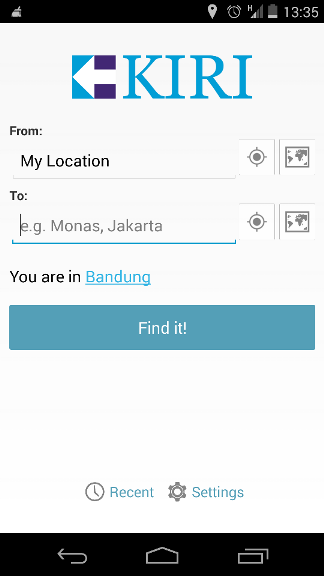
\includegraphics[scale=0.5]{Gambar/KIRI_Android/home}
	\caption{Tampilan Utama Aplikasi Public Transport}
	\label{fig:home}
\end{figure}

Gambar ~\ref{fig:home} menunjukan halaman utama aplikasi Public Transport. Di halaman ini pengguna dapat memasukan lokasi asal dan lokasi tujuan. Cara memasukan lokasi ada 2 macam yaitu dengan mengetik dan menunjuk pada peta dengan mengetuk tombol peta. Bila pengguna ingin menunjuk lokasi pengguna berada dapat dilakukan dengan menunjuk lokasi pada peta lalu menekan tombol untuk memilih koordinat. Tersedia juga pilihan kota yang dapat dipilih oleh pengguna.

\begin{figure}[h]
	\centering
		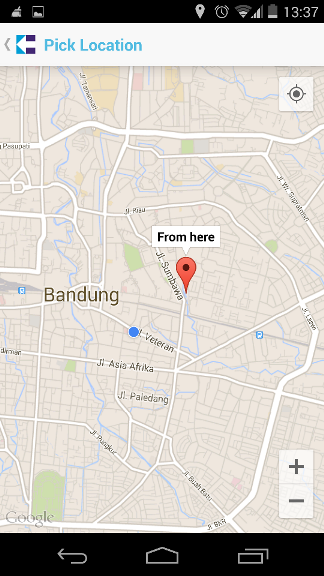
\includegraphics[scale=0.5]{Gambar/KIRI_Android/menunjuk_lokasi}
	\caption{Menunjuk Lokasi pada Peta}
	\label{fig:menunjuk}
\end{figure}

Gambar ~\ref{fig:menunjuk} jika pengguna sudah mengetahui lokasi namun tidak tahu nama lokasi. Pada halaman ini pengguna diarahkan untuk menemukan lokasi pada peta memilihnya.

\begin{figure}[h]
	\centering
		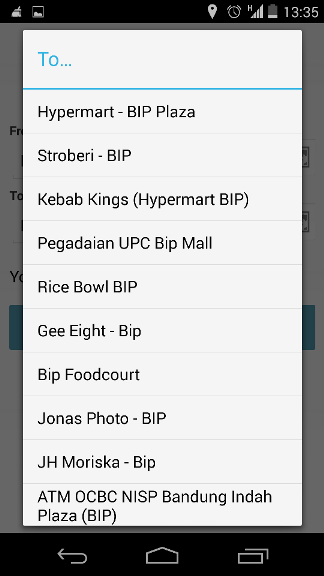
\includegraphics[scale=0.5]{Gambar/KIRI_Android/terkait}
	\caption{Memberikan Daftar Nama Tempat dan Nama Jalan Terkait}
	\label{fig:terkait}
\end{figure}

Pada gambar ~\ref{fig:terkait} pengguna dapat memilih nama tempat terkait. Pemilihan didasarkan sesuai masukan pengguna untuk memastikan tempat asal maupun tempat tujuan. Jika nama tempat sudah jelas maka tidak ada halaman yang menampilkan nama tempat.

\begin{figure}[h]
	\centering
		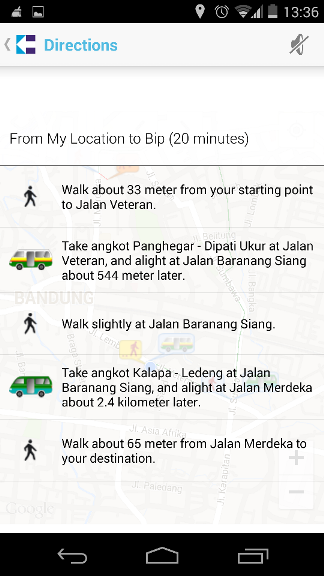
\includegraphics[scale=0.5]{Gambar/KIRI_Android/tampilan_daftar}
	\caption{Tampilan Rute Kendaraan Umum dalam Bentuk Daftar}
	\label{fig:daftar}
\end{figure}

Pada gambar ~\ref{fig:daftar} menampilkan daftar rute kendaraan umum yang harus dinaiki beserta gambar untuk mempermudah pengguna. Selain itu disertakan juga jarak dan perkiraan waktu sampai di lokasi tujuan.

\begin{figure}[h]
	\centering
		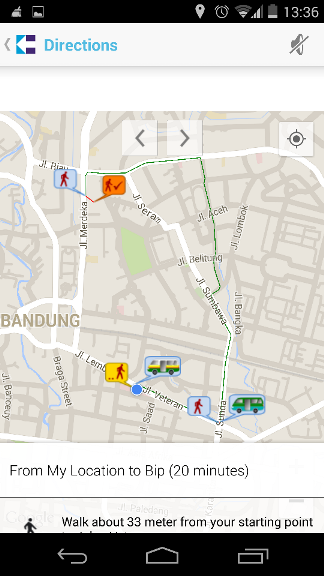
\includegraphics[scale=0.5]{Gambar/KIRI_Android/tampilan_peta}
	\caption{Tampilan Rute Kendaraan Umum di Peta}
	\label{fig:peta}
\end{figure}
\newpage
Pada gambar ~\ref{fig:peta} menampilkan rute kendaraan umum dan jalur yang harus dilalui pada peta. Dengan cara ini pengguna dapat mengetahui posisi dan jalur yang harus dilalui.

% tampilannya, cara kerja, hal yang dapat dilakukan

%Analisis Analisis Program
\section{Analisis Aplikasi}
\label{lab:Analisis Aplikasi}
\hspace{0.5cm} Aplikasi dibuat menggunakan bahasa pemograman C\#. Aplikasi yang digunakan untuk membangun Aplikasi Pencari Rute Kendaraan Umum untuk Windows Phone adalah Visual Studio Express 2012. Pada sub-bab ini dibahas kebutuhan aplikasi, anaslisis kontrol yang dipakai, analisis terhadap siklus hidup aplikasi, analisis peta, analisis pemanfaatan sumber data, analisa Kiri API, diagram \textit{use case}, dan diagram kelas dari aplikasi yang dibangun. 

%Analisis Kebutuhan Aplikasi
\subsection{Kebutuhan Aplikasi}
\label{lab:Kebutuhan Aplikasi}
\hspace{0.5cm} Dari hasil observasi dalam menentukan lokasi asal dan lokasi tujuan ada dua cara. Kedua cara tersebut yaitu dengan menulis alamat atau tempat dan dengan menunjuk pada peta. Cara menuliskan alamat atau tempat yaitu dengan menuliskan alamat atau tempat pada tempat yang disediakan untuk asal dan tujuan. Cara menunjuk pada peta yaitu dengan menunjuk peta pada koordinat yang diinginkan. Kedua hal tersebut pada dasarnya sama saja tetapi ada faktor kemudahan pengguna dalam pemakaiannya. Jadi aplikasi menyediakan dua cara tersebut dengan tujuan agar pengguna dapat memilih salah satunya.

Pada saat menuliskan lokasi atau tempat atau menunjuk langsung pada peta mungkin saja terjadi kesalahan. Kesalahan tersebut bisa saja disebabkan salah pengetikan atau nama tempat yang tidak ada. Maka dari itu dibutuhkan pemeriksaan terhadap masukan pengguna. Pemeriksaan tersebut dilakukan setelah pengguna memulai pencarian dengan menekan tombol "FIND".

Untuk hasil keluaran ada dua tipe seperti aplikasi peta lainnya. Kedua tipe tersebut adalah bentuk daftar dan bentuk peta. Bentuk daftar memudahkan dalam melihat tiap langkah rute. bentuk peta memudahkan pengguna dalam melihat arah dan posisi lingkungan pada rute yang dipilih.

\hspace{0.5cm} Berdasarkan kebutuhan aplikasi diatas maka aplikasi yang dibangun didasarkan pada kebutuhan sebagai berikut.
\begin{enumerate}
	\item Pengguna dapat memasukan lokasi asal dan lokasi tujuan pada \textit{textbox} yang disediakan atau menunjuk langsung lokasi pada peta.
	\item Mendapatkan lokasi terkait menurut lokasi yang dimasukan pengguna.
	\item Menampilkan hasil rute angkutan umum dari lokasi asal ke lokasi tujuan.
\end{enumerate}

% SUB Analisis Kontrol yang Dipakai
\subsection{Analisis Kontrol yang Dipakai}
\label{lab:Analisis Kontrol yang Dipakai}
\hspace{0.5cm} Dari kebutuhan yang telah disebutkan diatas disadari pentingnya kontrol yang harus dipakai. Kontrol yang dimaksud termasuk tata letak, teks, pilihan, dan daftar. Kebutuhan kontrol penting bukan hanya untuk kebutuhan tapi memudahkan pengguna.

Untuk kontrol tata letak dibutuhkan pengaturan yang tertata rapih dan beberapa elemen dalam satu baris atau kolom. Penggunaan kontrol tata letak yang rumit tidak diharapkan dalam aplikasi karena akan membingungkan pengguna. Dari hasil pengamatan kontrol tata letak yang cocok adalah tata letak \textit{grid}. Kontrol tata letak ini dipilih karena mudah diposisiskan sesuai baris dan kolom. Kelebihan tata letak \textit{grid} adalah menyesuaikan jika layar diputar dari posisi pemandangan ke posisi potret dan sebaliknya.

Kontrol terhadap teks juga diperlukan untuk aplikasi. Kebutuhan yang diperlukan adalah mengeluarkan potongan teks yang dapat dibaca dan tempat pengguna memasukan teks. Untuk mengeluarkan teks yang dapat dilihat pengguna diperlukan penggunakan \textit{textblock}. \textit{textblock} digunakan untuk menampilkan tulisan "from" dan "to" pada halaman utama aplikasi. Untuk masukan pengguna, aplikasi menyediakan \textit{textbox} sebagai tempat masukan teks. \textit{textbox} digunakan sebagai masukan untuk lokasi asal dan lokasi tujuan.

Suatu aplikasi tentunya tidak hanya mempunyai satu halaman, aplikasi yang dibuat memiliki beberapa halaman yang mempunyai tugas berbeda. Karena hal tersebut dibutuhkan kontrol untuk berpindah dari satu halaman ke halaman lain. Kontrol yang dibutuhkan yaitu kontrol tombol. Kontrol tombol mengeksekusi \textit{event click} yang memungkinkan pindah halaman dan melakukan perintah. Kontrol tombol digunakan untuk berpindah ke halaman peta, menemukan lokasi pengguna, dan pencarian rute. Pada halaman utama terdapat 5 buah dengan penjelasan sebagai berikut.
\begin{itemize}
	\item Tombol "map" pada bagian from\\
	Tombol untuk berpindah dari halaman utama menuju halaman peta. Pada halaman peta pengguna dapat menunjuk lokasi asal dan kembali lagi ke halaman utama. Saat kembali ke halaman utama lokasi yang dipilih akan disimpan dan pada \textit{TextBox} bagian from akan tertulis "Maps".
	\item Tombol "here" pada bagian from\\
	Tombol untuk mancari lokasi pengguna. Setelah tombol ini di tekan maka lokasi pengguna akan disimpan dan pada bagian \textit{TextBox} bagian from akan tertulis "Here".
	\item Tombol "map" pada bagian to\\
	Tombol untuk berpindah dari halaman utama menuju halaman peta. Pada halaman peta pengguna dapat menunjuk lokasi tujuan dan kembali lagi ke halaman utama. Saat kembali ke halaman utama lokasi yang dipilih akan disimpan dan pada \textit{TextBox} bagian to akan tertulis "Maps".
	\item Tombol "here" pada bagian to\\
	Tombol untuk mancari lokasi pengguna. Setelah tombol ini di tekan maka lokasi pengguna akan disimpan dan pada bagian \textit{TextBox} bagian to akan tertulis "Here".
	\item Tombol find\\
	Tombol ini akam mencari rute angkutan umum dan menampilkannya pada halaman peta.
\end{itemize}

Pada aplikasi ini ditampilkan daftar tempat dan daftar rute angkutan umum yang dipakai. Bentuk daftar digunakan karena hasil tempat dan rute angkutan umum yang ditampilkan cukup banyak jumlahnya. Bentuk daftar yang dapat dipakai di Windows Phone adalah menggunakan \textit{ListBox}. \textit{ListBox} menampilkan daftar tempat dan daftar rute satu per satu menurun ke bawah.

% SUB Analisis Terhadap Siklus Hidup Aplikasi
\subsection{Analisis Terhadap Siklus Hidup Aplikasi}
\label{lab:Analisis Terhadap Siklus Hidup Aplikasi}
\hspace{0.5cm} Aplikasi pada Windows Phone memiliki siklus hidup yang dijelaskan pada bab ~\ref{subsec:Siklus Hidup Aplikasi}. Pengaturan aplikasi ini diatur sesuai konfigurasi awal sistem operasi Windows Phone. Tetapi pengaturan ini dapat diatur sesuai kebutuhan aplikasi. Karena di aplikasi ini terdapat keadaan yang berbeda dengan konfigurasi awal sistem operasi Windows Phone maka perlu dilakukan pengaturan ulang siklus hidup.

Saat aplikasi dijalankan, pengguna memasukkan lokasi asal dan lokasi tujuan. Setelah memasukkan lokasi pengguna lalu mencari rute. Ketika rute berhasil ditemukan maka aplikasi berada di keadaan Running. Tetapi ada kemungkinan pengguna berpindah aplikasi atau mematikan layar untuk menghemat daya. Dalam kasus tersebut sistem operasi Windows Phone menganggap aplikasi tidak aktif dan aplikasi masuk pada keadaan \textit{dormant}. Untuk menangani kasus tersebut maka aplikasi harus menyimpan keadaan dan informasi sesaat sebelum aplikasi menjadi tidak aktif. Penanganan yang digunakan adalah menyimpan keadaan sebelumnya di memori.

Pada saat aplikasi masuk keadaan Dormant semua \textit{thread} dan proses akan dihentikan. Pada saat tersebut juga GPS Windows Phone terhenti dan tidak akan mengetahui posisi pengguna. GPS akan kembali aktif mengetahui posisi pengguna jika pengguna masuk ke aplikasi dan tentunya membutuhkan waktu untuk pelacakan lokasi. Tetapi Windows Phone mendukung proses di belakang untuk pelacakan GPS selama keluar dari aplikasi atau layar perangkat dimatikan. Maka dari itu aplikasi yang dibuat harus mendukung pengaksesan lokasi meskipun layar perangkat dimatikan atau berpindah aplikasi. 

Ketika aplikasi sudah berada pada keadaan \textit{Dormant} atau \textit{Tombstoned}, pengguna masih dapat memulihkan keadaan aplikasi saat aplikasi berada di keadaan \textit{Running} sebelumnya. Penanganan yang dilakukan untuk hal tersebut adalah menggunakan \textit{method} OnNavigatedTo(). Menggunakan \textit{method} tersebut bertujuan memulihkan informasi halaman pada keadaan \textit{Running} sebelumnya.
%mendukung backgorund execution, running bacground event

% SUB Analisis Peta
\subsection{Analisis Peta}
\label{lab:Analisis Peta}
\hspace{0.5cm} Untuk tampilan peta ada beberapa aspek yang perlu diperhatikan untuk memudahkan pengguna. Aspek yang perlu diperhatikan adalah sebagai berikut.
\begin{itemize}
	\item Pemetaan terhadap peta atau \textit{cartographic} dan mode warna
	\item Tingkat \textit{zoom}
	\item Menampilkan gambar dan keterangan angkutan umum menggunakan \textit{pushpin}
	\item Menggambar rute pada peta menggunakan \textit{polyline}
\end{itemize}

Untuk cara pandang peta terdapat 4 pandangan yang disediakan peta di Windows Phone yaitu \textit{Road}, \textit{Aerial}, \textit{Hybrid}, dan \textit{Terrain}. Aplikasi ini adalah aplikasi pencari rute dan pandangan lebih banyak diarahkan ke jalanan perkotaan. Kebutuhan pengguna adalah nama jalan, kondisi jalan, dan kondisi sekitar. Dari dasar pandangan tersebut pandangan yang dipilih untuk aplikasi ini adalah \textit{Road}. Tambahan setelah mengatur pandangan peta yaitu mengatur warna dan menggunakan mode warna terang sesuai bawaan peta di Windows Phone.

Tampilan awal peta di Windows Phone akan mengeluarkan peta dengan pandangan dunia. Karena aplikasi pencarian rute ini masih terbatas di Pulau Jawa, Indonesia terutama Jawa Barat maka tingkat \textit{zoom} harus diatur agar mengikuti lokasi pengguna dan di satu daerah saja. Jika pengguna berada di daerah Bandung maka tingkat \textit{zoom} pada peta disesuaikan pada daerah tersebut. Tingkat \textit{zoom} dapat dapat diatur dari kode dan XAML. Tingkat \textit{zoom} yang digunakan adalah 14. Tingkat \textit{zoom} 14 menampilkan satu kota dengan jelas.
%kasih gambar zoom 14

Di setiap kota ada satu angkutan umum yang banyak dipakai yaitu angkutan kota(angkot). Namun bagi yang baru pertama mengunjungi suatu daerah dan mencari angkot mungkin akan mengalami kesulitan membaca trayek/rute dari angkot tersebut. Namun ada satu cara yang mudah untuk membedakan angkot di setiap rute yaitu dari warna dan coraknya. Agar dapat memudahkan pengguna dan menghindari pengguna dari kesalahan naik angkot maka Kiri API sudah menyediakan gambar angkot yang seusai dengan setiap rute. Gambar angkot tersebut akan ditempatkan di peta dengan suatu penampung beserta keterangannya. Salah satu teknik untuk menempatkan gambar tersebut adalah dengan membuat lapisan terpisah di atas peta tempat gambar tersebut. Untuk hal tersebut dimanfaatkan \textit{pushpin} sebagai lapisan terpisah untuk menaruh gambar dan keterangan angkutan umum. Berikut tampilan \textit{pushpin} untuk angkot~\ref{fig:pushpin_angkot} dan \textit{pushpin} untuk jalan kaki~\ref{fig:pushpin_jalan}.

\begin{figure}[h]
	\centering
		
\includegraphics[scale=0.5]{Gambar/out_kiri/angkot}
	\caption{Tampilan \textit{Pushpin} untuk Angkot}
	\label{fig:pushpin_angkot}
\end{figure}

\begin{figure}[h]
	\centering
		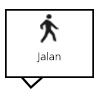
\includegraphics[scale=0.5]{Gambar/out_kiri/jalan}
	\caption{Tampilan \textit{Pushpin} untuk Jalan Kaki}
	\label{fig:pushpin_jalan}
\end{figure}

Pencarian rute yang digunakan untuk aplikasi yaitu dengan memakai Kiri API. Kiri API memberikan kembalian berupa titik-titik rute perjalanan dari lokasi asal ke lokasi tujuan. Karena hal itu aplikasi harus menggambar rute tersebut sesuai jalan pada peta. Untuk hal tersebut digunakan \textit{polyline} pada Windows Phone untuk menggambarnya. \textit{Polyline} yang digambar harus terlihat dengan jelas dan diberi warna yang kontras dengan tampilan peta. Warna polyline yang dipilih adalah merah dengan ketebalan 4.

% SUB Analisis Pemanfaatan Sumber Data
\subsection{Analisis Pemanfaatan Sumber Data}
\label{lab:Analisis Pemanfaatan Sumber Data}
\hspace{0.5cm} Aplikasi yang dibuat memanfaatkan sumber data dari luar. Sumber data yang didapatkan dalam format JSON (\textit{Javascript object Notation}). Pengambilan sumber data tersebut dilakukan dengan melakukan permintaan melalui protokol HTTP dengan parameter \textit{Uniform Resource Identifier} / URI. 

Untuk dapat memanfaatkan sumber data di Windows Phone perlu memanfaatkan kelas HttpClient.\textit{Method} yang digunakan adalah GetStringAsync(). \textit{Method} ini mengirimkan permintaan dengan parameter URI dan hasil yang dikembalikan memiliki tipe data \textit{string}. Karena \textit{method} ini mengembalikan hasil dalam tipe data \textit{string} maka mudah disesuaikan dengan kebutuhan tugas akhir ini. Selanjutnya agar data dalam bentuk \textit{string} tersebut dapat dimanfaatkan maka diperlukan proses \textit{Deserialization}. Proses \textit{Deserialization} dimaksudkan untuk mengubah bentuk \textit{string} ke objek. Untuk melakukan \textit{Deserialization} perlu memanfaatkan \textit{library} Json.NET. Aplikasi memanfaatkan \textit{library} Json.NET karena memiliki performa yang baik. Untuk hal tersebut aplikasi yang dibuat perlu menggunakan \textit{method} DeserializeObject().
%penggunaan getString

% SUB Analisis Kiri API
\subsection{Analisis Kiri API}
\label{lab:Analisis Kiri API}
%parameter get karena hanya untuk mendapatkan data dan tidak ada data sensiti yg dikirimkan.
\hspace{0.5cm} Kiri API menyediakan 2 jenis permintaan yaitu \textit{POST} dan \textit{GET}. Dalam tugas akhir ini digunakan protokol \textit{GET} untuk melakukan permintaan. Permintaan \textbf{GET} dipilih karena dalam tugas akhir ini aplikasi banyak mendapatkan data dan tidak ada data sensitif yang dikirimkan. Untuk hal ini maka mengirim ke URI \url{http://kiri.travel/handle.php}.

Untuk setiap permintaan terhadap Kiri API dibutuhkan \textit{API key}. Kegunaan \textit{API key} adalah password untuk mengakses Kiri API. \textit{API key} dapat didapatkan di \url{dev.kiri.travel}. \textit{API key} yang digunakan pada tugas akhir ini adalah 97A7A1157A05E***. %97A7A1157A05ED6F
     
Untuk tugas akhir ini digunakan 2 layanan yang ada pada Kiri API. Layanan yang digunakan adalah pencarian lokasi dan penentuan rute. Pencarian lokasi adalah layanan untuk menemukan tempat atau nama jalan yang terkait dengan masukan pengguna. Penentuan rute adalah layanan untuk menemukan langkah yang harus ditempuh pengguna untuk sampai ke lokasi tujuan dari lokasi asal. 

Pemanfaatan layanan pencarian lokasi yaitu dengan parameter \textit{GET} melalui protokol HTTP. Berikut parameter yang harus dikirimkan beserta keterangannya.
\begin{itemize}
	\item \textit{version}: 2 \\
	Karena acuan yang digunakan adalah Kiri API versi 2 maka di parameter version aplikasi menggunakan versi 2.
	\item \textit{mode}: "searchplace" \\
	Mode "searchplace" digunakan untuk mencari lokasi terkait.
	\item \textit{region}: "cgk" untuk Jakarta, "bdo" untuk Bandung, dan "sub" untuk Surabaya \\
	Karena Kiri API baru tersedia di 3 kota yaitu Jakarta, Bandung, dan Surabaya maka region harus dimasukan untuk pencarian. Region harus dipilih antara "cgk"/"bdo"/"sub" sebagai parameter. Pengguna dapat menentukan masukan region jika menuliskannya pada lokasi asal atau lokasi tujuan. Tetapi, jika pengguna tidak menuliskannya maka sistem yang akan menentukan. Cara penentuan region oleh sistem adalah sistem akan menampung titik tengah dari ketiga region tersebut lalu membandingkannya dengan lokasi pengguna berada. Jarak terdekat antara lokasi pengguna dan salah satu region menandakan pengguna berada di region tersebut.
	\item \textit{querystring}: merupakan kata kunci lokasi 
	\item \textit{apikey}: 16 digit heksadesimal
\end{itemize}
Format layanan yang dikirim melalui URL adalah \url{kiri.travel/handle.php?version=2&mode=searchplace&region=cgk/bdo/sub&querystring="string"&apikey=97A7A1157A05E***}.
\newline
\\Percobaan mencari lokasi bip dari kata kunci "bip" yang berada di bandung. Layanan dikirimkan ke URL \url{kiri.travel/handle.php}. 
Berikut format layanan yang dikirimkan:\newline
{\url{http://kiri.travel/handle.php?version=2&mode=searchplace&region=bdo&querystring=bip&apikey=97A7A1157A05E***}}
\newline
\\Berikut hasil kembalian dari Kiri API: 

\begin{lstlisting} [caption= Kode Kembalian dari Pencarian Rute]
{ 
	"status":"ok",
	"searchresult":[
		{
			"placename":"Hypermart - BIP Plaza",
			"location":"-6.90864,107.61108"
		},
		{
			"placename":"Stroberi - BIP",
			"location":"-6.90834,107.61115"
		},
		{
			"placename":"Kebab Kings (Hypermart BIP)",
			"location":"-6.91503,107.61017"
		},
		{
			"placename":"Pegadaian UPC Bip Mall",
			"location":"-6.90916,107.61052"
		},
		{
			"placename":"Rice Bowl BIP",
			"location":"-6.90873,107.61088"
		},
		{	
			"placename":"Gee Eight - Bip",
			"location":"-6.90817,107.61080"
		},
		{
			"placename":"Jonas Photo - BIP",
			"location":"-6.91066,107.61016"
		},
		{
			"placename":"Bip Foodcourt",
			"location":"-6.91081,107.61015"
		},
		{
			"placename":"Mister Baso BIP",
			"location":"-6.90348,107.61709"
		},
		{
			"placename":"JH Moriska - Bip",
			"location":"-6.90868,107.61070"
		}
	],
	"attributions":null
}
\end{lstlisting}

Hasil dari kembalian berupa kumpulan \textit{placename} dan \textit{location}. Hasil tersebut ditampung aplikasi, namun yang ditampilkan ke pengguna hanya \textit{placename}. Menampilkan \textit{location} tidak efektif karena akan membingungkan pengguna. Dari percobaan yang dilakukan, nilai dari \textit{attributions} selalu bernilai "null". Karena hal tersebut maka nilai \textit{attributions} diabaikan.

Layanan lainnya yang dimanfaatkan adalah layanan penentuan rute. Pemanfaatan layanan penentuan rute digunakan mendapatkan langkah-langkah yang harus ditempuh pengguna untuk menuju lokasi tujuan dari lokasi asal. Pemanfaatan layanan ini yaitu dengan permintaan \textit{GET} melalui protokol HTTP. Berikut parameter yang harus dikirim:
\begin{itemize}
	\item \textit{version}: 2 \\
	Karena acuan adalah Kiri API versi 2 maka pada parameter versi ditulis 2.
	\item \textit{mode}: "findroute" \\
	Mode "findroute" digunakan untuk mendapatkan langkah yang harus ditempuh menuju lokasi tujuan.
	\item \textit{locale}: "en" untuk bahasa Inggris dan "id" untuk bahasa Indonesia. \\
	Karena aplikasi ini bertujuan untuk memudahkan pemakaian transportasi di Indonesia maka diputuskan untuk menggunakan bahasa Indonesia.
	\item \textit{start}: koordinat lokasi asal dalam bentuk \textit{string} bernilai \textit{latitude} dan \textit{longitude} yang dipisahkan koma. \\
	Masukan untuk lokasi awal harus dalam bentuk kordinat. Jika masukan dari pengguna adalah alamat atau tempat maka perlu dicari kordinatnya dahulu.
	\item \textit{finish}: koordinat lokasi tujuan dalam bentuk \textit{string} bernilai \textit{latitude} dan \textit{longitude} yang dipisahkan koma. \\
	Masukan untuk lokasi tujuan harus dalam bentuk kordinat. Jika masukan dari pengguna adalah alamat atau tempat maka perlu dicari kordinatnya dahulu.
	\item \textit{presentation}: "mobile" untuk perangkat \textit{mobile} dan "desktop" untuk komputer. \\
	Karena aplikasi ini dirancang untuk Windows Phone 8, presentasi yang dipilih adalah "desktop". Pemilihan ini didasarkan karena deskripsi yang ditampilkan tidak ada tulisan "image from" dan "image to", selain itu presentasi "desktop" juga memungkinkan rute alternatif. 
	\item \textit{apikey}: 16 digit heksadesimal.
\end{itemize}

Format layanan yang dikirim melalui URL adalah \url{kiri.travel/handle.php?version=2&mode=findroute&locale=en/id&start=lat,lng&finish=lat,lng&presentation=mobile/desktop&apikey=97A7A1157A05ED6}

Percobaan pernentuan rute menuju Jalan Merdeka dari Jalan Ciumbuleuit. Layanan dikirimkan ke URL \url{kiri.travel/handle.php}. Format layanan yang dikirim dengan \textit{presentation mobile} adalah \url{http://kiri.travel/handle.php?version=2&mode=findroute&locale=id&start=-6.8747337,107.6048829&finish=-6.9114646,107.6104887&presentation=mobile&apikey=97A7A1157A05ED6F}.
\newline
Berikut hasil kembalian dari Kiri API:
\begin{lstlisting} [caption= Kode Kembalian Pencarian Rute dengan \textit{Presentation Mobile}]
{
	"status":"ok",
	"routingresults":[
		{
			"steps":[
				[
					"walk",
					"walk",
					["-6.8747337,107.6048829","-6.87445,107.60465"],
					"Jalan dari lokasi mulai Anda \%fromicon ke Jalan Ciumbuleuit \%toicon sejauh kurang lebih 41 meter.",
					null,
					null
				],
				[
					"angkot",
					"ciumbuleuitsthalllurus",
					["-6.87445,107.60465","-6.87541,107.60443","-6.87637,107.60421","-6.87734,107.60400",
					"-6.87830,107.60378", "-6.87926,107.60356","-6.87926,107.60356","-6.87963,107.60352",
					"-6.87978,107.60352","-6.88093,107.60392","-6.88209,107.60433","-6.88209,107.60433",
					"-6.88328,107.60490","-6.88328,107.60490","-6.88347,107.60481","-6.88452,107.60459",
					"-6.88556,107.60436","-6.88660,107.60413","-6.88764,107.60390","-6.88764,107.60391",
					"-6.88782,107.60392","-6.88887,107.60404","-6.88991,107.60416","-6.88991,107.60416",
					"-6.89161,107.60428","-6.89161,107.60428","-6.89166,107.60421","-6.89275,107.60424",
					"-6.89275,107.60424","-6.89405,107.60408","-6.89405,107.60408","-6.89496,107.60400"],
					"Naik angkot Ciumbuleuit - St. Hall (lurus) di Jalan Ciumbuleuit \%fromicon, dan turun di Jalan Cihampelas \%toicon kurang lebih setelah 3,3 kilometer.",
					null,
					https:\/\/angkot.web.id\/go\/route\/640?ref=kiri
				],
				[
					"walk",
					"walk",
					["-6.90424,107.60433","-6.90429,107.60440"],
					"Jalan dari Jalan Cihampelas \%fromicon ke Jalan Abdul Rivai \%toicon sejauh kurang lebih 10 meter.",
					null,
					null
				],
				[
					"angkot",
					"kalapaledeng",
					["-6.89501,107.60403","-6.89562,107.60398","-6.89623,107.60395","-6.89732,107.60401",
					"-6.89732,107.60401","-6.89882,107.60414","-6.89882,107.60414","-6.89969,107.60418",
					"-6.90071,107.60426","-6.90173,107.60433","-6.90173,107.60433","-6.90297,107.60437",
					"-6.90420,107.60440","-6.90420,107.60440","-6.90426,107.60456","-6.90422,107.60481",
					"-6.90399,107.60546","-6.90406,107.60617","-6.90454,107.60697","-6.90454,107.60697",
					"-6.90512,107.60745","-6.90618,107.60778","-6.90618,107.60778","-6.90643,107.60787",
					"-6.90651,107.60807","-6.90675,107.60914","-6.90675,107.60914","-6.90694,107.60939",
					"-6.90723,107.60939","-6.90891,107.60943","-6.90891,107.60943","-6.90909,107.60934",
					"-6.90914,107.60857","-6.90933,107.60846","-6.91021,107.60887","-6.91021,107.60887",
					"-6.91030,107.60897","-6.91028,107.60927","-6.90986,107.61040","-6.90986,107.61040"],
					"Naik angkot Kalapa - Ledeng di Jalan Abdul Rivai \%fromicon, dan turun di Jalan Aceh \%toicon kurang lebih setelah 1,1 kilometer.",
					"https:\/\/angkot.web.id\/go\/route\/156?ref=kiri"
				],
				[
					"walk",
					"walk",
					["-6.90986,107.61040","-6.9114646,107.6104887"],
					"Walk about 178 meter from Jalan Aceh \%fromicon to your destination \%toicon.",
					null,
					null
				]
				],
					"traveltime":"30 minutes"
				}
			]
}
\end{lstlisting}

Format layanan yang dikirim dengan \textit{presentation desktop} adalah \\
\url{http://kiri.travel/handle.php?version=2&mode=findroute&locale=id&start=-6.8747337,107.6048829&finish=-6.9114646,107.6104887&presentation=desktop&apikey=97A7A1157A05ED6F}.

Berikut hasil kembalian dari Kiri API:
\begin{lstlisting} [caption= Kode Kembalian Pencarian Rute dengan \textit{Presentation Desktop}]
{
	"status":"ok",
	"routingresults":[
		{
			"steps":[
				[
					"walk",
					"walk",
					["-6.8747337,107.6048829","-6.87445,107.60464"],
					"Jalan dari lokasi mulai Anda ke Jalan Ciumbuleuit sejauh kurang lebih 41 meter.",
					null,
					null
				],
				[
					"angkot",
					"ciumbuleuitsthalllurus",
					["-6.87445,107.60464","-6.87541,107.60443","-6.87541,107.60443","-6.87637,107.60422",
					"-6.87637,107.60422","-6.87734,107.60400","-6.87734,107.60400","-6.87830,107.60378",
					"-6.87830,107.60378","-6.87926,107.60356","-6.87926,107.60356","-6.87926,107.60356",
					"-6.87963,107.60352","-6.87978,107.60352","-6.88093,107.60393","-6.88093,107.60393",
					"-6.88209,107.60433","-6.88209,107.60433","-6.88209,107.60433","-6.88328,107.60490",
					"-6.88328,107.60490","-6.88328,107.60490","-6.88347,107.60481","-6.88452,107.60458",
					"-6.88452,107.60458","-6.88556,107.60435","-6.88556,107.60435","-6.88660,107.60413",
					"-6.88660,107.60413","-6.88764,107.60390","-6.88764,107.60390","-6.88764,107.60390",
					"-6.88782,107.60392","-6.88887,107.60404","-6.88887,107.60404","-6.88991,107.60416",
					"-6.88991,107.60416","-6.88991,107.60416","-6.89161,107.60428","-6.89161,107.60428",
					"-6.89161,107.60428","-6.89166,107.60420","-6.89275,107.60424","-6.89275,107.60424",
					"-6.89275,107.60424","-6.89405,107.60407","-6.89405,107.60407","-6.89405,107.60407",
					"-6.89496,107.60400","-6.89496,107.60400","-6.89586,107.60392","-6.89586,107.60392",
					"-6.89586,107.60392","-6.89759,107.60397","-6.89759,107.60397","-6.89759,107.60397",
					"-6.89895,107.60406","-6.89895,107.60406","-6.89895,107.60406","-6.89970,107.60413",
					"-6.89999,107.60416","-6.90114,107.60426","-6.90114,107.60426","-6.90114,107.60426",
					"-6.90218,107.60428","-6.90218,107.60428","-6.90321,107.60431","-6.90321,107.60431",
					"-6.90424,107.60433"],
					"Naik angkot Ciumbuleuit - St. Hall (lurus) di Jalan Ciumbuleuit, dan turun di Jalan Cihampelas kurang lebih setelah 3,3 kilometer.",
					null,
					"https:\/\/angkot.web.id\/go\/route\/640?ref=kiri"
				],
				[
					"walk",
					"walk",
					["-6.90424,107.60433","-6.90429,107.60440"],
					"Jalan dari Jalan Cihampelas ke Jalan Abdul Rivai sejauh kurang lebih 10 meter.",
					null,
					null
				],
				[
					"angkot",
					"kalapaledeng",
					["-6.90429,107.60440","-6.90434,107.60490","-6.90398,107.60558","-6.90417,107.60619",
					"-6.90465,107.60702","-6.90465,107.60702","-6.90465,107.60702","-6.90521,107.60748",
					"-6.90600,107.60771","-6.90646,107.60775","-6.90755,107.60760","-6.90755,107.60760",
					"-6.90755,107.60760","-6.90866,107.60789","-6.90866,107.60789","-6.90866,107.60789",
					"-6.90911,107.60826","-6.91034,107.60892","-6.91034,107.60892","-6.91034,107.60892",
					"-6.91007,107.60985"],
					"Naik angkot Kalapa - Ledeng di Jalan Abdul Rivai, dan turun di Jalan Aceh kurang lebih setelah 1,1 kilometer.",
					null,
					"https:\/\/angkot.web.id\/go\/route\/156?ref=kiri"
				],
				[
					"walk",
					"walk",
					["-6.91007,107.60985","-6.9114646,107.6104887"],
					"Jalan dari Jalan Aceh ke tujuan akhir Anda sejauh kurang lebih 171 meter.",
					null,
					null
				]],
				"traveltime":"30 menit"}]}
\end{lstlisting}

Setiap langkah kembalian dari Kiri API ditampung dalam elemen \textit{array}. Untuk keterangan dan jenis angkutan umum aplikasi tampilkan dalam bentuk \textit{pushpin} pada peta atau daftar. Sedangkan untuk titik-titik kordinat digambarkan pada peta. Dari analisa didapatkan bahwa setiap langkah menunjukan perpindahan angkutan umum yang dipakai, berpindah dari angkutan umum atau jalan, dan dari jalan untuk menaiki angkutan umum. Keterangan yang ditambahkan harus berada antara setiap \textit{steps} tersebut. Dari analisa didapatkan kata "\%fromicon" dan "\%toicon" yang tidak menunjukan sesuatu untuk keluaran jika melakukan permintaan dengan \textit{presentation mobile}. Karena hal tersebut mode \textit{presentation} yang digunakan adalah \textit{desktop}. Gambar angkutan kota dan gambar jalan yang sudah disediakan dari Kiri diambil dengan memanfaatkan URL yang disediakan. 

%Analisis Diagram Use-Case dan Skenario
\subsection{Diagram \textit{Use Case} dan Skenario}
\label{lab:Diagram Use-Case dan Scenario}
\hspace{0.5cm} Diagram \textit{use case} adalah diagram yang menjelaskan interaksi sistem dengan lingkungan (contoh: pengguna). Berdasarkan analisa di atas maka pengguna dapat:
\begin{itemize}
	\item Mendapatkan lokasi pengguna berada.
	\item Memasukan lokasi asal dan lokasi tujuan.
	\item Menunjuk langsung lokasi asal dan tujuan pada peta.
	\item Memilih alamat atau tempat dari pilihan yang disediakan.
	\item Menampilkan rute kendaraan umum dalam bentuk titik dan \textit{pushpin} pada peta atau bentuk daftar dari tempat asal ke tempat tujuan.
\end{itemize}

\newpage
Diagram \textit{use case} saat pengguna mencari rute kendaraan umum dapat dilihat pada gambar (Gambar:~\ref{fig:UseCase}):
% Use case
\begin{figure}[h]
	\centering
		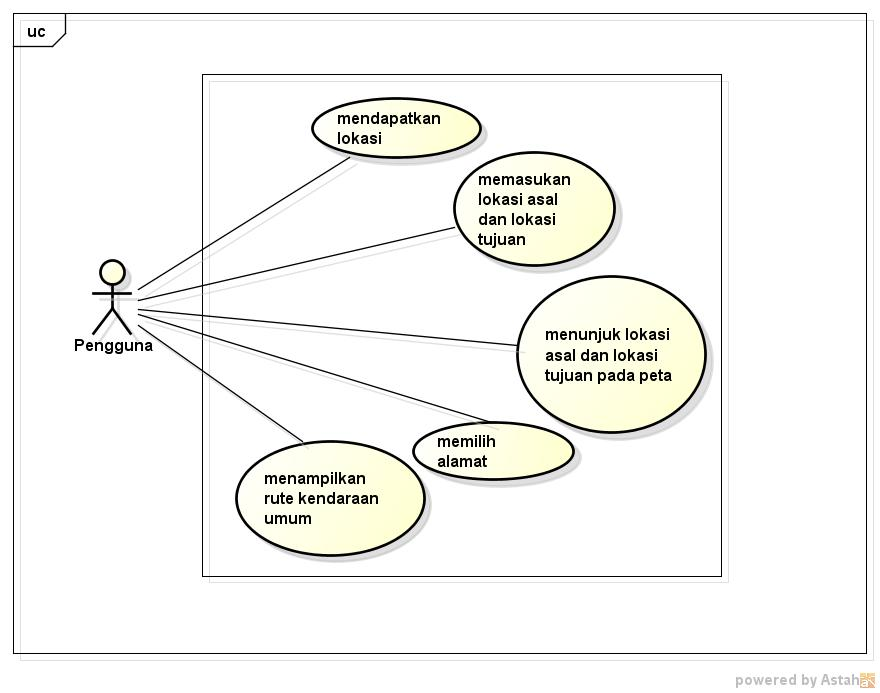
\includegraphics[scale=0.5]{Gambar/useCase_dan_Class/UseCase}
	\caption{Diagram \textit{Use Case}}
	\label{fig:UseCase}
\end{figure}

Skenario pencarian rute kendaraan umum dapat dilihat pada tabel~\ref{tab:mandapatLokasi} sampai tabel~\ref{tab:menampilkan}.
%\vtop{\hbox{\strut kalimat_1} \hbox{\strut kalimat_2}}
\begin{table}[H]
	\centering
		\begin{tabular}{ |p{2cm}|p{10cm}| }
			\hline
			Nama &  Mendapatkan lokasi perangkat\\ \hline
			Aktor & Pengguna  \\ \hline
			Deskripsi & Mendapatkan lokasi perangkat berada  \\ \hline
			Kondisi awal & \textit{textbox} masih kosong dan pengguna menekan tombol lokasi \\ \hline
			Kondisi akhir & Lokasi ditemukan dan \textit{textbox} berisi "here" \\ \hline
			Skenario utama & Pengguna menekan tombol lalu perangkat mencari lokasi perangkat dan \textit{textbox} berisi "here" \\ \hline
			Eksespsi & Lokasi tidak ditemukan jika GPS perangkat tidak aktif  \\ 
			\hline
		\end{tabular}
	\caption{Skenario Mendapatkan Lokasi untuk Masukan Lokasi Asal dan Lokasi Tujuan}
	\label{tab:mandapatLokasi}
\end{table}

\begin{table}[H]
	\centering
		\begin{tabular}{ |p{2cm}|p{10cm}| }
			\hline
			Nama &  Masukan pada \textit{textbox}\\ \hline
			Aktor & Pengguna  \\ \hline
			Deskripsi & Memasukan lokasi asal pengguna dan tujuan pengguna(masukan dapat berupa alamat, kordinat, atau tempat) \\ \hline
			Kondisi awal & \textit{textbox} masih dalam keadaan belum terisi \\ \hline
			Kondisi akhir & Lokasi awal dan tujuan sudah dimasukan   \\ \hline
			Skenario utama & Pengguna mengetikan lokasi awal dan tujuan pada \textit{textbox} yang sudah disediakan \\ \hline
			Eksespsi & Tidak ada  \\ 
			\hline
		\end{tabular}
	\caption{Skenario Memasukan Lokasi Asal dan Lokasi Tujuan pada \textit{textbox}}
	\label{tab:masukanLokasi}
\end{table}

\begin{table}[H]
	\centering
		\begin{tabular}{ |p{2cm}|p{10cm}| }
			\hline
			Nama &  Menunjuk lokasi pada peta\\ \hline
			Aktor & Pengguna  \\ \hline
			Deskripsi & Memasukan lokasi asal pengguna dan tujuan pengguna dengan menunjuk pada peta \\ \hline
			Kondisi awal & \textit{textbox} masih dalam keadaan belum terisi \\ \hline
			Kondisi akhir & \textit{textbox} terisi dengan "Maps"   \\ \hline
			Skenario utama & Pengguna menunjuk lokasi pada peta dan \textit{textbox} terisi dengan "Maps" \\ \hline
			Eksespsi & Tidak ada  \\ 
			\hline
		\end{tabular}
	\caption{Skenario Menunjuk Lokasi Asal dan Lokasi Tujuan pada Peta}
	\label{tab:lokasiPeta}
\end{table}

\begin{table}[H]
	\centering
		\begin{tabular}{ |p{2cm}|p{10cm}| }
			\hline
			Nama &  Memilih alamat\\ \hline
			Aktor & Pengguna  \\ \hline
			Deskripsi & Pengguna memilih alamat atau lokasi yang terkait masukan pengguna \\ \hline
			Kondisi awal & Lokasi awal dan lokasi tujuan terisi dan pengguna menekan tombol "Find" \\ \hline
			Kondisi akhir & Pengguna sudah memilih dan lokasi sudah dapat dipastikan  \\ \hline
			Skenario utama & Pengguna menekan tombol "Find". Sistem mengembalikan daftar yang berisi alamat atau tempat terkait masukan pengguna \\ \hline
			Eksespsi & Lokasi masukan pengguna tidak ditemukan  \\ 
			\hline
		\end{tabular}
	\caption{Skenario Memilih Alamat}
	\label{tab:memilihAlamat}
\end{table}

\begin{table}[H]
	\centering
		\begin{tabular}{ |p{2cm}|p{10cm}| }
			\hline
			Nama &  Menampilkan rute kendaraan umum\\ \hline
			Aktor & Pengguna  \\ \hline
			Deskripsi & Lokasi dari pengguna diolah menjadi rute kendaraan umum dari lokasi asal dan lokasi tujuan \\ \hline
			Kondisi awal & Lokasi sudah dapat dipastikan \\ \hline
			Kondisi akhir & Rute kendaraan umum dimunculkan pada peta dan dalam bentuk daftar \\ \hline
			Skenario utama & Lokasi dapat dipastikan sistem lalu istem akan memproses data masukan. Sistem akan mengembalikan hasil rute kendaraan umum pada peta dan dalam bentuk daftar \\ \hline
			Eksespsi & Rute kendaraan umum tidak ditemukan  \\ 
			\hline
		\end{tabular}
	\caption{Skenario Menampilkan Rute Kendaraan Umum}
	\label{tab:menampilkan}
\end{table}

%Analisis Kelas Diagram
\subsection{Kelas Diagram}
\label{lab:Kelas Diagram}
\hspace{0.5cm} Pembuatan kelas diagram didasarkan pada skenario pada sub-bab~\ref{lab:Diagram Use-Case dan Scenario}. Kelas diagram dapat dilihat pada gambar~\ref{fig:kelas}.

% Kelas
\begin{figure}[h]
	\centering
		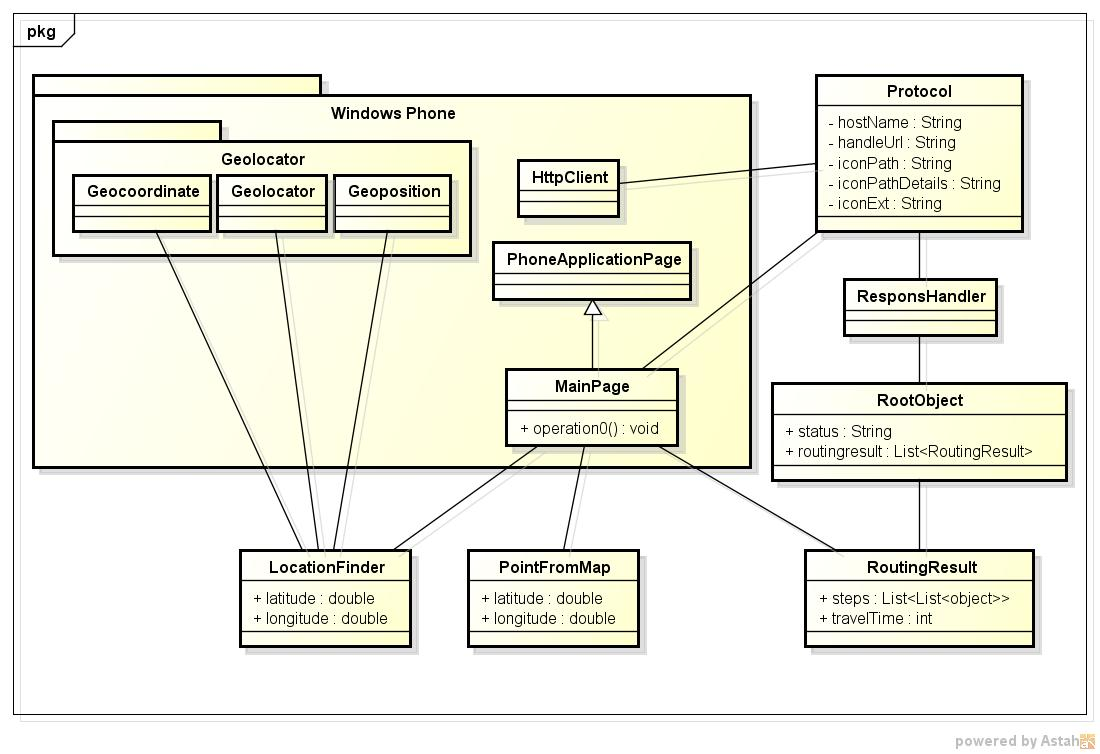
\includegraphics[scale=0.4]{Gambar/useCase_dan_Class/class}
	\caption{Diagram Kelas}
	\label{fig:kelas}
\end{figure}

Berikut deskripsi kelas pada gambar~\ref{fig:kelas}.
\begin{itemize}
	\item Kelas Protocol \\
	Merupakan kelas yang menampung semua alamat URL yang berhubungan dengan Kiri API. Semua pemanggilan ditangani oleh kelas ini.
	\item Kelas ResponsHandler \\
	Merupakan kelas yang menangani masukan dari pemanggilan layanan.
	\item Kelas RootObject \\
	Merupakan kelas untuk menampung status dan daftar dari layanan \textit{routing} Kiri API. Hasil kembalian dipisahkan di kelas ini untuk selanjutnya ditampung di kelas \textit{RoutingResult}. 
	\item Kelas RoutingResult \\
	Merupakan kelas untuk menampung setiap langkah dari rute sesuai masukan pengguna. Pada kelas ini juga rute digambarkan pada peta.
	\item Kelas PointFromMap \\
	Merupakan kelas yang dapat mengetahui lokasi yang ditunjuk pengguna pada peta. Kelas ini menyimpan lokasi yang ditunjuk pengguna dalam bentuk \textit{latitude} dan \textit{longitude}.
	\item Kelas LocationFinder \\
	Merupakan kelas yang digunakan untuk mencari lokasi. Kelas ini memanfaatkan kelas \textit{Geocoordinate} untuk mendapatkan lokasi. Setelah lokasi didapatkan dalam bentuk kelas \textit{Geoposition} maka diubah ke \textit{latitude} dan \textit{longitude}. 
\end{itemize}}{}
\ifdefstring{\vbabd}{1}{\chapter{Perancangan}
\label{chap:Perancangan}

Pada bab 4 akan dibahas mengenai perancangan seperti diagram \textit{sequence}, diagram kelas secara rinci, deskripsi artibut dan \textit{method} dari setiap kelas, dan perancangan antarmuka.

%Perancangan Diagram Sequence
\section{Diagram \textit{Sequence}}
\label{lab:Diagram Sequence}
\hspace{0.5cm} Diagram \textit{sequence} merupakan diagram yang menggambarkan interkasi antar objek dalam suatu skenario. Gambar diagram \textit{sequence} dapat dilihat pada gambar ~ref{fig:sequence lokasi perangkat} sampai ~ref{fig:sequence rute}. 

% Sequence mendapat lokasi perangkat
\begin{figure}[h]
	\centering
		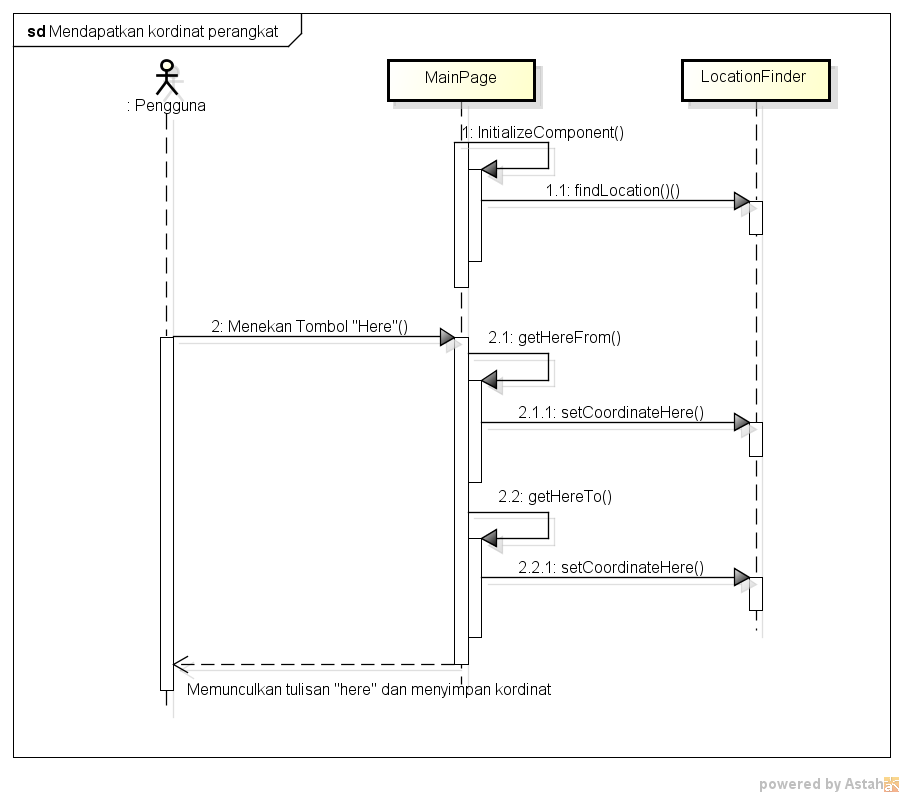
\includegraphics[scale=0.4]{Gambar/sequence/MendapatkanKordinatPerangkat}
	\caption{Diagram \textit{sequence} Mendapatkan Kordinat perangkat}
	\label{fig:sequence lokasi perangkat}
\end{figure}

\hspace{0.5cm} Diagram ~\ref{fig:sequence lokasi perangkat} merupakan diagram \textit{sequence} untuk memilih lokasi dengan lokasi perangkat berada. Diagram menunjukan bahwa setelah aplikasi dibuka maka aplikasi akan mencari dahulu lokasi perangkat dengan memanfaatkan kelas LocationFinder. Lalu setelah aplikasi terbuka jika pengguna ingin memilih lokasi tersebut sebagai lokasi asal maka pengguna harus menekan tombol "here". Setelah tombol "here" ditekan maka kelas MainPage akan mengambil nilai \textit{Latitude} dan nilai \textit{Longitude} dari kelas LocatonFinder. Setelah lokasi didapatkan maka akan muncul tulisan "here" pada masukan di kelas MainPage.

% Sequence mendapat lokasi dari peta
\begin{figure}[h]
	\centering
		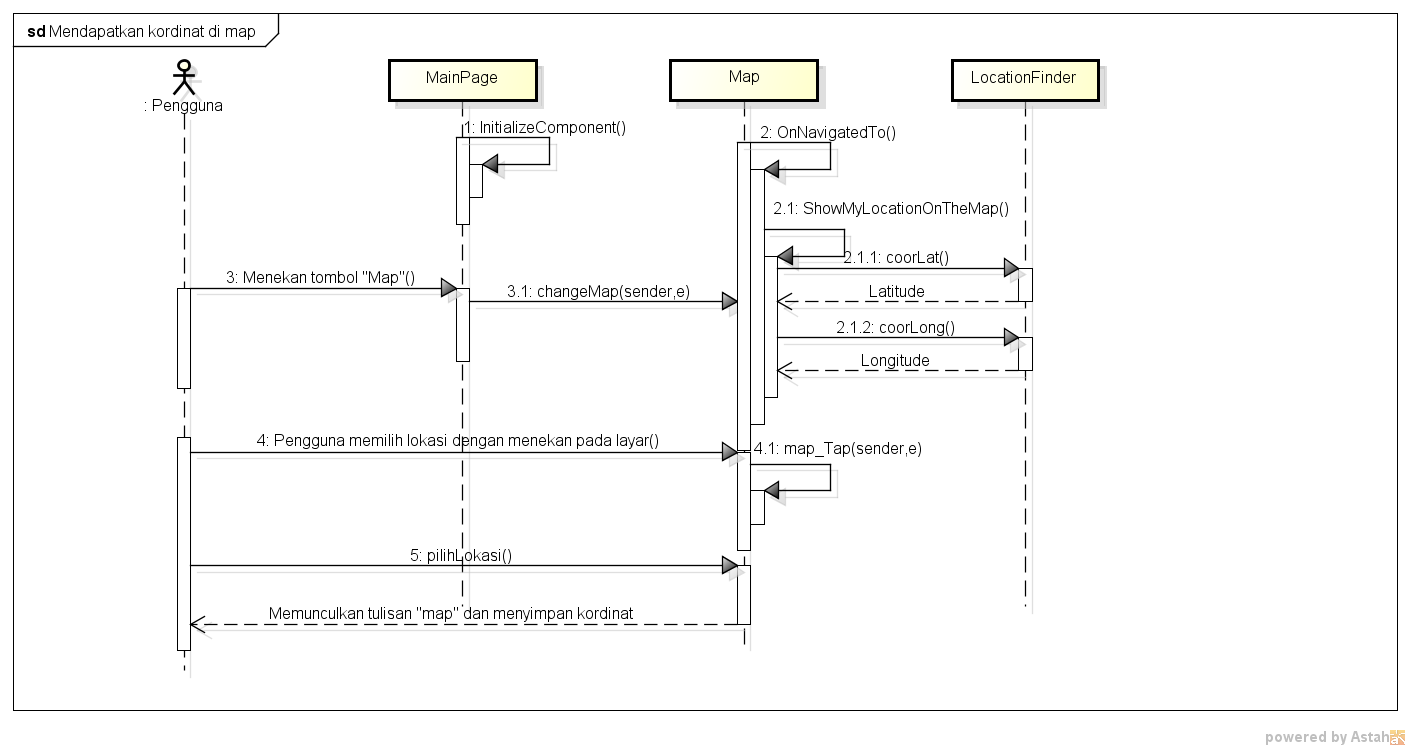
\includegraphics[scale=0.4]{Gambar/sequence/MendapatkanKordinatDiMap}
	\caption{Diagram \textit{sequence} Mendapatkan Kordinat pada Peta}
	\label{fig:sequence lokasi pada peta}
\end{figure}

\hspace{0.5cm} Diagram ~\ref{fig:sequence lokasi pada peta} merupakan diagram \textit{sequence} untuk memilih lokasi. Diagram menunjukan bahwa setelah aplikasi dibuka maka pengguna dapat menekan tombol "map". Setelah tombol "map" ditekan maka halaman akan dialihkan ke kelas Map. Saat kelas Map terbuka maka lokasi yang ditunjukan adalah lokasi dimana perangkat berada. Untuk mengetahui lokasi kelas Map mengambil kordinat \textit{latitude} dan \textit{longitude} dari kelas LocationFinder. Di kelas "Map" pengguna dapat memilih lokasi dengan memilih lokasi pada peta dan memanggil \textit{method map\_tap}, lalu setelah pengguna memilih tempat pengguna akan menekan tombol Pilih Lokasi yang akan memanggil \textit{method pilihLokasi}. Lokasi yang dipilih pengguna akan disimpan di kelas MainPage dan pada masukan akan tertulis "map". 

\hspace{0.5cm} Diagram ~\ref{fig:sequence rute} merupakan diagram \textit{sequence} untuk mencari rute. Diagram menunjukan bahwa setelah aplikasi dibuka maka aplikasi akan melakukan inisialisasi. Untuk mencari rute dari lokasi asal ke lokasi tujuan dibutuhkan kordinat \textit{latitude} lokasi asal, \textit{longitude} lokasi asal, \textit{latitude} lokasi tujuan, dan \textit{longitude} lokasi tujuan. Jika pengguna mendapatkan lokasi dari peta atau sesuai lokasi maka yang didapatkan sudah pasti kordinat, namun jika pengguna memasukan kata kunci perlu didapat kordinat \textit{latitude} dan \textit{longitude} dari kata kunci tersebut. Jika masukan yang didapat berupa kata kunci maka akan dilakukan pemeriksaan apakah kordinat untuk kata kunci tersebut tersedia. Pemeriksaan dilakukan dengan melakukan pemanggilan Kiri API. Tahap pemanggilan meliputi pemangilan \textit{method GetStringAsync} lalu mengjadikan objek kembaliannya dengan \textit{method Deselialize}. Jika sudah didapat dan hasilnya lebih dari satu maka akan dipanggil \textit{method getListItem} yang akan menampilkan daftar pilihan ke pengguna untuk dipilih. Pengguna dapat memilih tempat sesuai tempat asal maupun tujuan yang diinginkan. Setelah lokasi asal dan lokasi tujuan didapat maka kelas MainPage akan mengarahkan ke kelas Route untuk menampilkan hasilnya. Kelas Route akan memanggil \textit{method OnNavigatedTo} yang bertujuan untuk mendapatkan lokasi asal dan lokasi tujuan. Setelah itu akan memanggil \textit{method Find} lalu mengembalikan rute yang ditemukan kepada pengguna.

\newpage

% Sequence mendapat rute
\begin{figure}[h!]
	\centering
		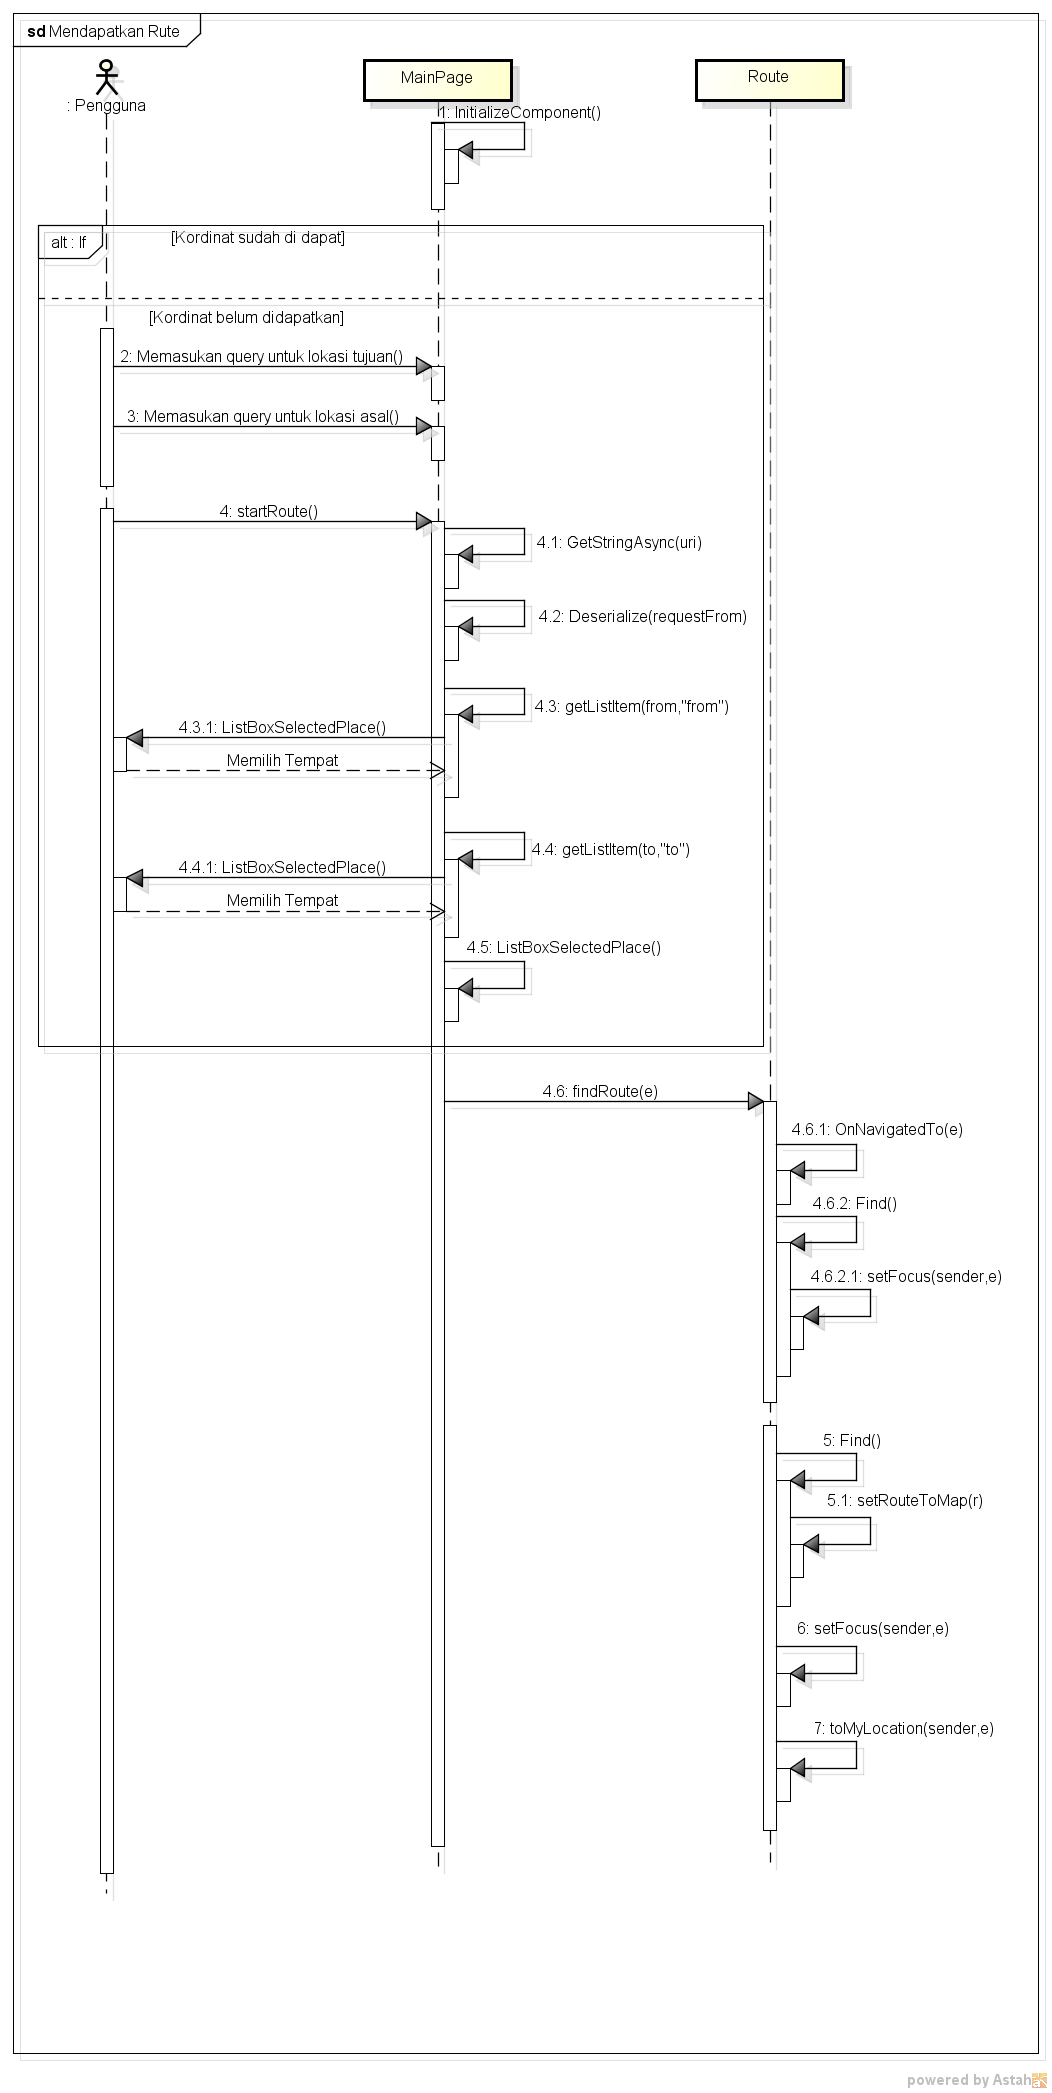
\includegraphics[scale=0.5]{Gambar/sequence/MendapatkanRute}
	\caption{Diagram \textit{sequence} Mendapatkan Rute}
	\label{fig:sequence rute}
\end{figure}


%Perancangan Kelas
\section{Perancangan Kelas}
\label{lab:Perancangan Kelas}
\hspace{0.5cm} Pada sub bab ini akan dibahas mengenai deskripsi kelas secara rinci pada aplikasi Pencari Rute Kendaraan Umum untuk Windows Phone. Untuk lebih jelas mengenai kelas yang ada pada aplikasi ini, penulis menyajikan gambar diagram kelas yang dapat dilihat pada  gambar ~\ref{fig:kelas}. 

% Kelas
\begin{figure}[h]
	\centering
		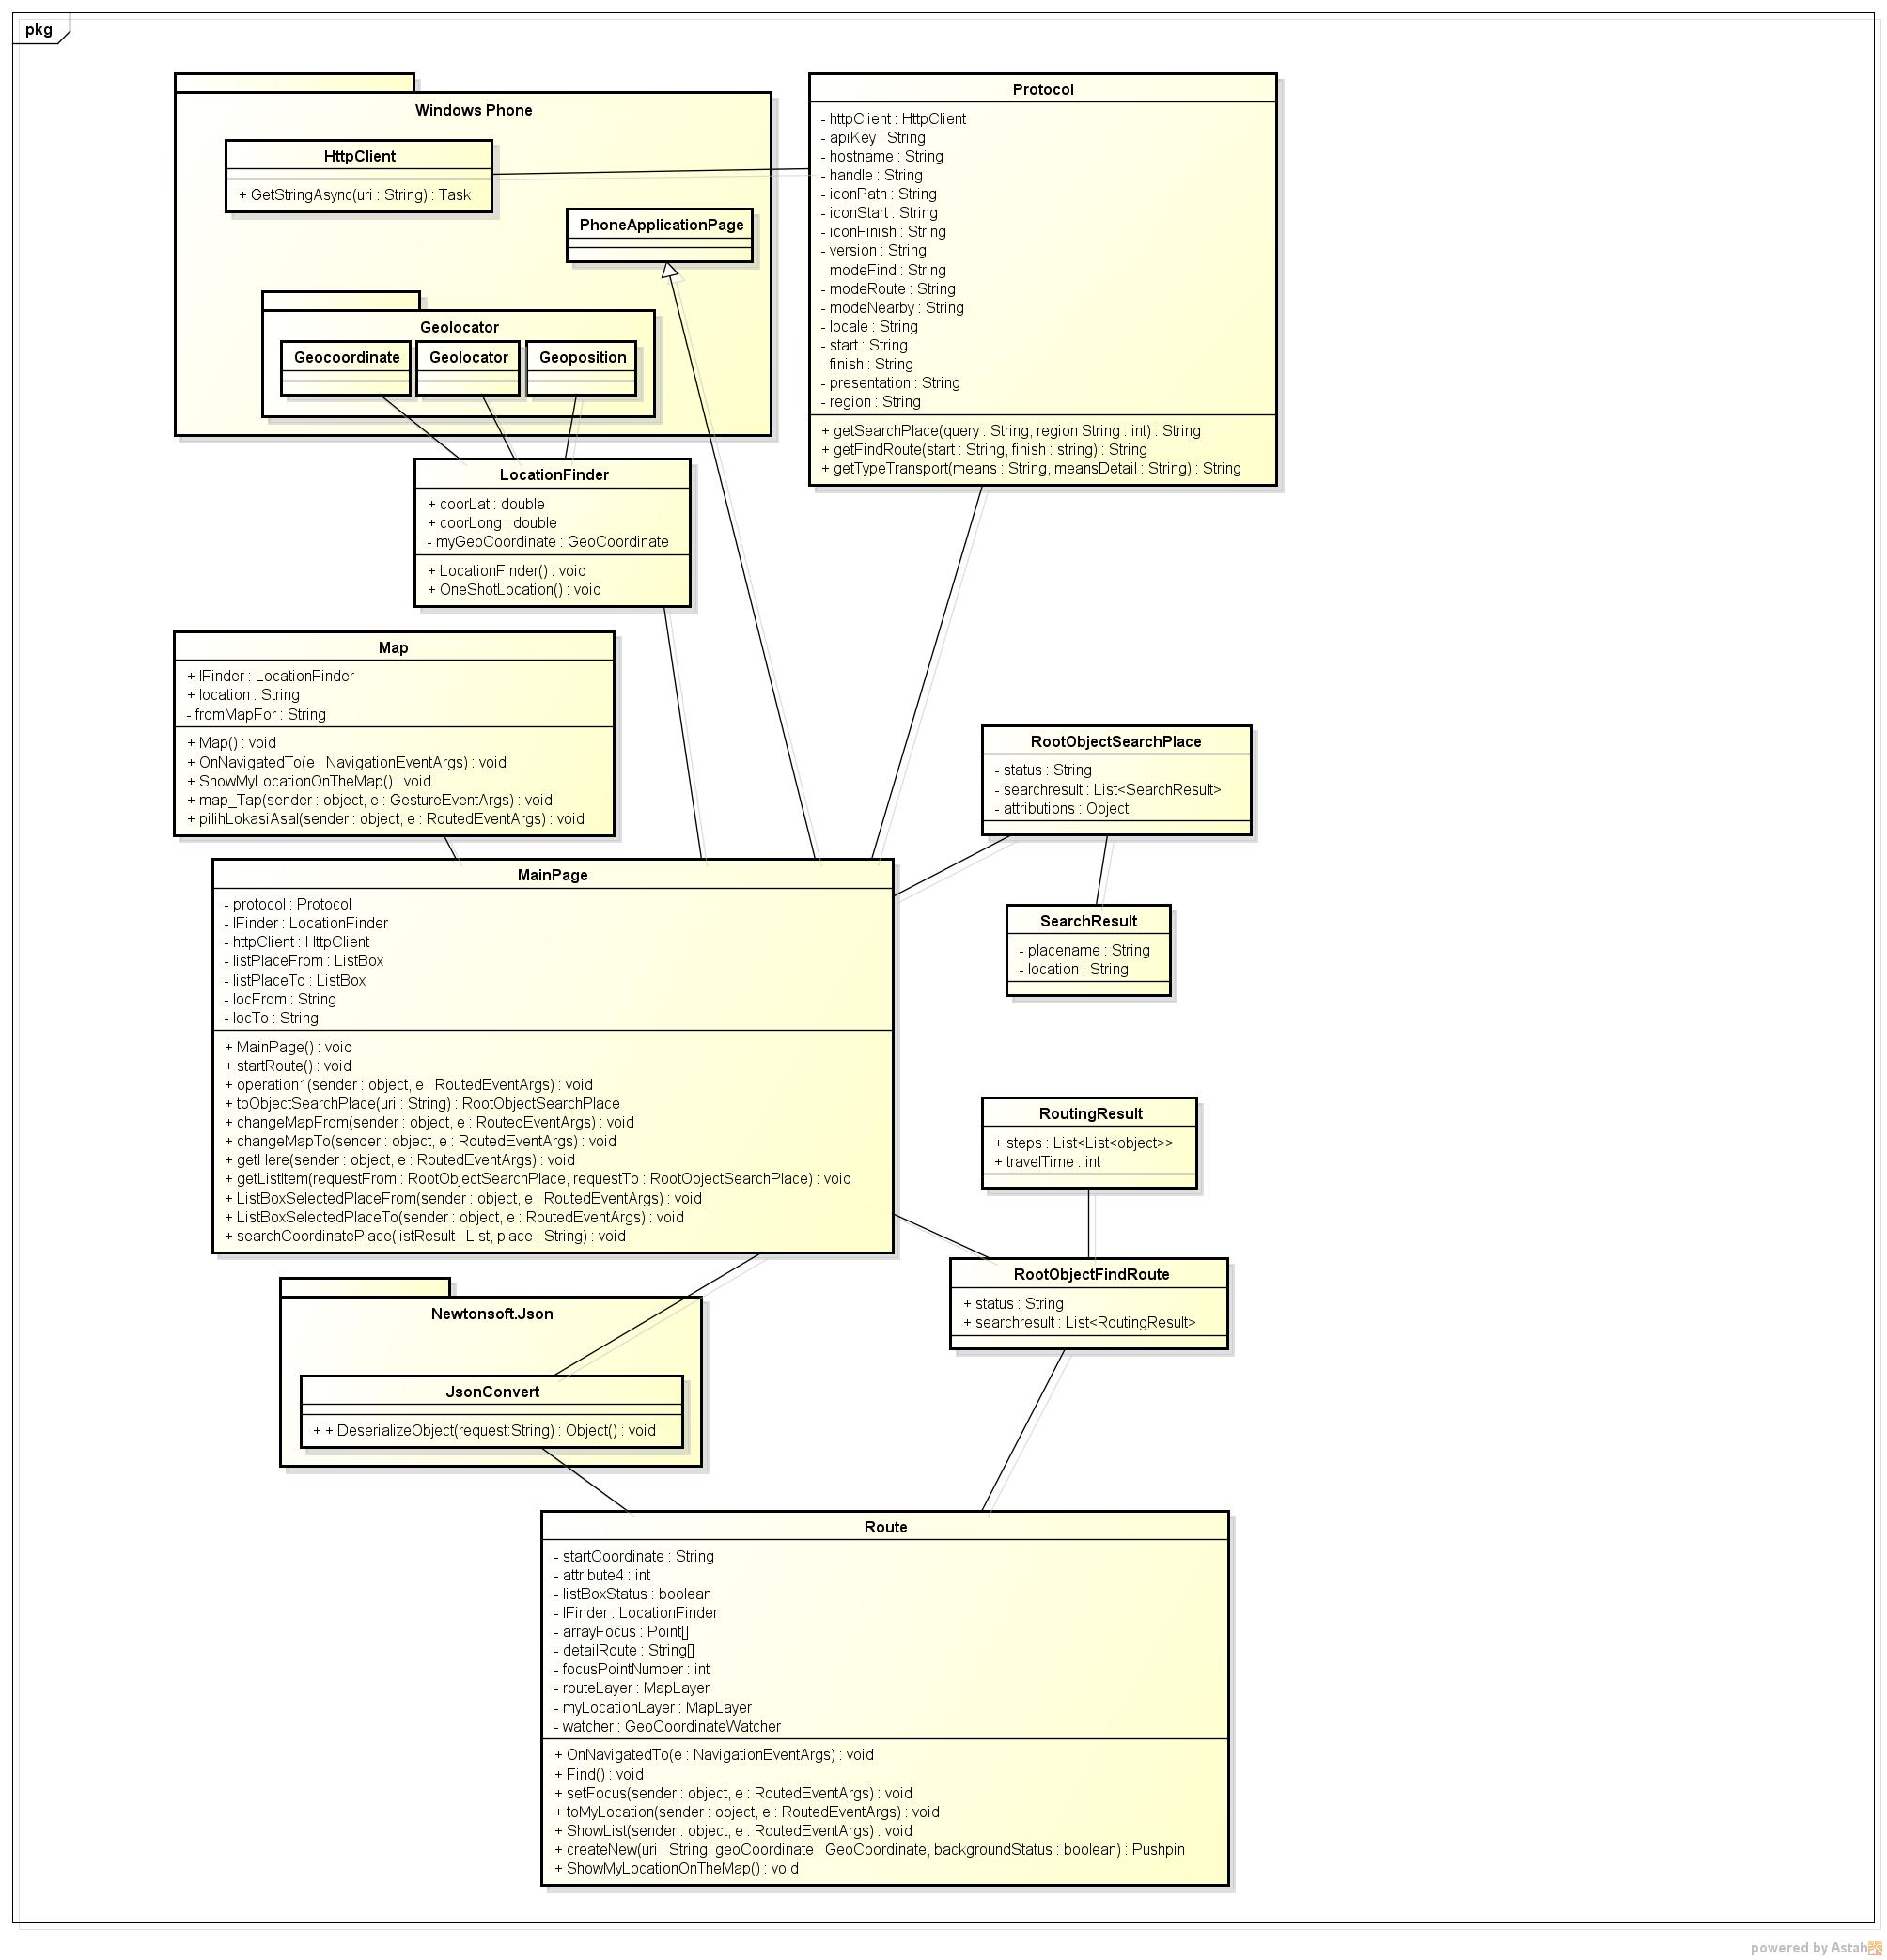
\includegraphics[scale=0.2]{Gambar/useCase_dan_Class/class4}
	\caption{Diagram Kelas}
	\label{fig:kelas}
\end{figure}


%Kelas PhoneApplicationPage
\subsection{Kelas \textit{PhoneApplicationPage}}
\label{lab:Kelas PhoneApplicationPage}
\hspace{0.5cm} \textit{PhoneApplicationPage} merupakan kelas bawaan Windows Phone yang menangani interksi pengguna dengan aplikasi dan siklus hidup aplikasi.

%Kelas MainPage
\subsection{Kelas \textit{MainPage}}
\label{lab:Kelas MainPage}
\hspace{0.5cm} \textit{MainPage} merupakan kelas turunan dari kelas \textit{PhoneApplicationPage} yang menangani interaksi langsung antara halaman aplikasi dengan pengguna. Pada kelas ini akan ditaruh kontrol yang diperlukan. Berikut adalah penjelasan atribut-atribut yang dimiliki kelas ini:
\begin{enumerate}
	\item protocol bertipe Protocol untuk mendapatkan URL yang digunakan dalam permintaan ke Kiri API.
	\item lFinder bertipe LocationFinder digunakan untuk menampung semua informasi mengenai lokasi.
	\item httpClient bertipe HttpClient merupakan objek yang akan mengurus permintaan dan kembalian dari Kiri API.
	\item city bertipe kumpulan String untuk menampung kota yang didukung oleh layanan Kiri.
	\item myCity bertipe String untuk menampung kode kota sesuai Kode Penerbangan IATA.
	\item backgroundWorker bertipe BackgroundWorker untuk mengurus pencarian lokasi di belakang layar.
\end{enumerate}

Berikut adalah penjelasan beberapa \textit{method} yang dimiliki kelas ini:
\begin{enumerate}
	\item Konstruktor MainPage digunakan untuk memuat komponen yang ada di halaman MainPage dan mendapatkan kota terdekat dari lokasi perangkat.
	\item \textit{method} OnNavigatedTo digunakan untuk mendapatkan lokasi dari peta dan mendapatkan objek LocationFinder. \textit{Method} ini secara otomatis dipanggil jika pengguna kembali ke kelas MainPage. \textit{method} ini memiliki parameter NavigationEventArgs.
	\item \textit{method} OnNavigatedFrom digunakan untuk mengirimkan \textit{state} objek LocationFinder saat berpindah kelas. \textit{Method} ini secara otomatis dipanggil jika pengguna berpindah dari kelas MainPage ke kelas lain. \textit{method} ini memiliki parameter NavigationEventArgs.
	\item \textit{method} Application\_Deactivated digunakan untuk menyimpan \textit{state} objek saat meninggalkan aplikasi. \textit{method} ini memiliki parameter object dan DeactivatedEventArgs.
	\item \textit{method} Application\_Activated digunakan untuk mengambil \textit{state} objek saat kembali ke aplikasi. \textit{method} ini memiliki parameter object dan ActivatedEventArgs.
	\item \textit{method} startRoute digunakan untuk mendapatkan masukan pengguna. Jika masukan didapat dari peta atau lokasi perangkat berarti sudah dalam kordinat, namun jika masukan didapat dari \textit{query} maka akan dicari lokasi yang terkait sesuai \textit{query} tersebut. Lokasi terkait yang didapatkan akan dikembalikan ke pengguna untuk dipilih. Setelah pengguna lokasi dalam bentuk kordinat didapatkan maka kelas akan diarahkan ke kelas Route. \textit{method} ini memiliki parameter objek tombol dan event.
	\item \textit{method} changeMapFrom digunakan untuk berpindah ke halaman mapFrom. \textit{method} ini memiliki parameter objek tombol dan event.
	\item \textit{method} changeMapTo digunakan untuk berpindah ke halaman mapTo. \textit{method} ini memiliki parameter objek tombol dan event.
	\item \textit{method} getHereFrom digunakan untuk mendapatkan kordinat perangkat lalu menyimpan nilainya di kordinat asal di kelas LocationFinder dan menulisakan "Here" pada TextBox lokasi asal. \textit{method} ini memiliki parameter objek tombol dan event.
	\item \textit{method} getHereTo digunakan untuk mendapatkan kordinat perangkat lalu menyimpan nilainya di kordinat tujuan di kelas LocationFinder dan menulisakan "Here" pada TextBox lokasi tujuan. \textit{method} ini memiliki parameter objek tombol dan event.
	\item \textit{method} getListItem digunakan untuk membuat listBox lalu menampilkan ke pengguna. \textit{method} ini memiliki parameter RootObjectSearchPlace dan string yang menunjukan \textit{list} yang ditampilkan untuk lokasi asal dan lokasi tujuan. 
	\item \textit{method} ListBoxSelectedPlace digunakan untuk mendapatkan tempat asal yang dipilih pengguna. \textit{method} ini memiliki parameter objek dan \textit{event SelectionChangedEventArgs}. 
	\item \textit{method} searchCoordinatePlace digunakan untuk mencari kordinat dari tempat pilihan pengguna. \textit{method} ini memiliki parameter ListBox dan tempat yang dipilih dalam bentuk string.
	\item \textit{method} findRoute digunakan untuk berpindah ke kelas Route jika lokasi asal dan lokasi tujuan sudah ditentukan.
	\item \textit{method} changeCity digunakan untuk mengubah kota tujuan dari pencarian. \textit{method} ini memiliki parameter objek dan \textit{event SelectionChangedEventArgs}.
	\item \textit{method} showCity digunakan untuk mencari kota yang paling dekat dengan lokasi perangkat.
	\item \textit{method} ShowSplash digunakan untuk menampilkan tampilan awal untuk proses inisialisasi aplikasi.
	\item \textit{method} StartLoadingData digunakan untuk memanggil BackgroundWorker. BackgroundWorker digunakan untuk melakukan aksi di belakang layar.
	\item \textit{method} backgroundWorker\_DoWork digunakan untuk melakukan pemanggilan aksi di belakang layar. \textit{method} ini memiliki parameter objek dan DoWorkEventArgs.
	\item \textit{method} backgroundWorker\_RunWorkerCompleted digunakan untuk melakukan pemanggilan saat BackgroundWorker selesai melakukan tugasnya. \textit{method} ini memiliki parameter objek dan RunWorkerCompletedEventArgs.
\end{enumerate}

%Kelas City
\subsection{Kelas \textit{City}}
\label{lab:Kelas City}
\hspace{0.5cm} \textit{City} merupakan kelas yang menyimpan kota-kota yang mendukung pencarian rute kendaraam umum dengan bantuan Kiri. Berikut adalah penjelasan atribut-atribut yang dimiliki kelas ini:
\begin{enumerate}
	\item centerCity bertipe \textit{array of GeoCoordinate} untuk menyimpan kordinat pusat dari kota.
	\item city bertipe \textit{array of String} untuk menyimpan nama kota.
	\item cityCode bertipe \textit{array of String} untuk menyimpan kode kota dalam huruf kecil sesuai aturan IATA Airport Code. 
\end{enumerate}

Berikut adalah penjelasan beberapa \textit{method} yang dimiliki kelas ini:
\begin{enumerate}
	\item Konstruktor City digunakan untuk untuk inisialisasi nilai atribut.
	\item \textit{method} getNearby digunakan untuk mencari kota terdekat dengan lokasi perangkat. \textit{method} ini mengembalikan interger yang merupakan index kota pada atribut city. \textit{method} ini memiliki 2 buah parameter yaitu \textit{latitude} dan \textit{longitude} yang bertipe double.
	\item \textit{method} getIndexFromCityCode digunakan untuk mencari index pada \textit{array}  sesuai kode kota. \textit{method} ini memiliki parameter bertipe String yang merupakan kode kota.
\end{enumerate}

%Kelas BackgroundWorker
\subsection{Kelas \textit{BackgroundWorker}}
\label{lab:Kelas BackgroundWorker}
\hspace{0.5cm} \textit{BackgroundWorker} merupakan kelas yang dipakai untuk mengeksekusi operasi pada \textit{thread} terpisah. Berikut adalah penjelasan \textit{event} yang dimiliki kelas ini dan dipakai untuk perancangan aplikasi:
\begin{enumerate}
	\item \textit{Event} DoWork
	\item \textit{Event} RunWorkerCompleted
\end{enumerate}
Berikut adalah penjelasan beberapa \textit{method} yang dimiliki kelas ini:
\begin{enumerate}
	\item \textit{method} RunWorkerAsync digunakan untuk memulai operasi di belakang layar.
\end{enumerate}

%Kelas Geocoordinate
\subsection{Kelas \textit{Geocoordinate}}
\label{lab:Kelas Geocoordinate}
\hspace{0.5cm} \textit{Geocoordinate} merupakan kelas bawaan dari Windows Phone yang akan dimanfaatkan untuk membaca \textit{latitude} dan \textit{longitude}.

%Kelas Geolocator
\subsection{Kelas \textit{Geolocator}}
\label{lab:Kelas Geolocator}
\hspace{0.5cm} \textit{Geolocator} merupakan kelas bawaan Windows Phone untuk mengkases lokasi. Dengan bantuan kelas ini maka dapat mengetahui status lokasi dari perangkat dan menemukan lokasi secara akurat.

%Kelas Geoposition
\subsection{Kelas \textit{Geoposition}}
\label{lab:Kelas Geoposition}
\hspace{0.5cm} \textit{Geoposition} merupakan kelas yang menampung lokasi sesuak kembalian \textit{Geolocator}.

%Kelas LocationFinder
\subsection{Kelas \textit{LocationFinder}}
\label{lab:Kelas LocationFinder}
\hspace{0.5cm} \textit{LocationFinder} merupakan kelas yang akan menampung lokasi dan pencarian lokasi. Berikut adalah penjelasan atribut-atribut yang dimiliki kelas ini:
\begin{enumerate}
	\item coorLat bertipe Double untuk menampung kordinat latitude pengguna.
	\item coorLong bertipe Double untuk menampung kordinat longitude pengguna.
	\item coorLatFrom bertipe Double untuk menampung kordinat latitude lokasi asal yang diinginkan pengguna.
	\item coorLongFrom bertipe Double untuk menampung kordinat longitude lokasi asal yang diinginkan pengguna.
	\item coorLatTo bertipe Double untuk menampung kordinat latitude lokasi tujuan yang diinginkan pengguna.
	\item coorLongTo bertipe Double untuk menampung kordinat longitude lokasi tujuan yang diinginkan pengguna.
	
	\item addressDevice bertipe String untuk menyimpan alamat perangkat berada.
	\item addressDeviceFrom bertipe String untuk menyimpan alamat berdasarkan lokasi lokasi asal yang diinginkan pengguna.
	\item addressDeviceTo bertipe String untuk menyimpan alamat berdasarkan lokasi tujuan yang diinginkan pengguna.
	
	\item geolocator bertipe Geolocator untuk menampung pengaturan mendapatkan lokasi.
	\item myReverseGeocodeQuery bertipe ReverseGeocodeQuery untuk konversi dari alamat ke lokasi dan sebalikny.
	\item myCoordinate bertipe GeoCoordinate untuk menampung kordinat geografis.
	\item accuracy bertipe double untuk menampung akurasi perangkat mendapatkan lokasi.
\end{enumerate}

Berikut adalah penjelasan beberapa \textit{method} yang dimiliki kelas ini:
\begin{enumerate}
	\item Konstruktor LocationFinder berfungsi mengatur atribut geolocator dan mencari lokasi perangkat.
	\item \textit{method} findLocation berfungsi inisialisasi GPS lalu mendapat kordinat dan menampungnya di atribut.
	\item \textit{method} updateAccuracy berfungsi untuk mengubah nilai akurasi dari perangkat.
	\item \textit{method} setPositionChanged berfungsi mengubah atribut coorLat, atribut coorLong, dan akurasi jika terdapat perubahan lokasi. \textit{method} ini memiliki parameter Geolocator dan PositionChangedEventArgs yang akan menjalankan \textit{method} jika terdapat perubahan yang diberitahukan melalui kelas Geolocator.
	\item \textit{method} GetCurrentCoordinate berfungsi mengubah posisi saat ini, posisi lokasi asal, dan lokasi tujuan. \textit{method} ini memiliki tiga buah parameter \textit{latitude} bertipe Double, \textit{longitude} bertipe Double, dan paramFor bertipe String. Parameter \textit{latitude} dan \textit{longitude} merupakan lokasi sedangkan parameter paramFor digunakan sebagai tujuan perubahan lokasi. 
	\item \textit{method} ReverseGeocodeQueryFrom\_QueryCompleted berfungsi untuk mencari alamat lokasi asal. \textit{method} ini memiliki parameter objek dan QueryCompletedEventArgs<IList<MapLocation>>.
	\item \textit{method} ReverseGeocodeQueryTo\_QueryCompleted berfungsi untuk mencari alamat lokasi tujuan. \textit{method} ini memiliki parameter objek dan QueryCompletedEventArgs<IList<MapLocation>>.
	\item \textit{method} ReverseGeocodeQuery\_QueryCompleted berfungsi untuk mencari alamat lokasi perangkat. \textit{method} ini memiliki parameter objek dan QueryCompletedEventArgs<IList<MapLocation>>.
	\item \textit{method} setCoordinateHere berfungsi untuk menyimpan kordinat dan alamat perangkat ke kordinat dan alamat lokasi asal dan lokasi tujuan. \textit{method} ini memiliki parameter paramFor bertipe String yang akan digunakan sebagai masukan disimpannya lokasi perangkat.
	\item \textit{method} reset berfungsi untuk memasang kembali lokasi asal dan lokasi tujuan.
\end{enumerate}

%Kelas Map
\subsection{Kelas \textit{Map}}
\label{lab:Kelas Map}
\hspace{0.5cm} \textit{Map} merupakan kelas yang akan mendapatkan titik yang ditunjuk pengguna pada peta lalu menerjemahkannya dalam bentuk titik kordinat. Berikut adalah penjelasan atribut-atribut yang dimiliki kelas ini:
\begin{enumerate}
	\item lFinder bertipe LocationFinder digunakan untuk menampung semua informasi mengenai lokasi.
	\item fromMapFor bertipe string digunakan sebagai indikator lokasi asal atau lokasi tujuan yang didapatkan dari map.
\end{enumerate}

Berikut adalah penjelasan beberapa \textit{method} yang dimiliki kelas ini:
\begin{enumerate}
	\item Konstruktor Map untuk inisialisasi dan penambahan \textit{event} mengetuk pada peta.
	\item \textit{method} OnNavigatedTo berfungsi untuk mendapatkan masukan lokasi asal atau lokasi tujuan yang akan ditentukan dari map untuk kemudian ditampung di Objek LocationFinder. \textit{method} ini memiliki sebuah parameter NavigationEventArgs.
	\item \textit{method} OnNavigatedFrom digunakan untuk mengirimkan \textit{state} objek LocationFinder saat berpindah kelas. \textit{method} ini memiliki parameter NavigationEventArgs.
	\item \textit{method} ShowMyLocationOnTheMap digunakan untuk memberitahu dan menandai lokasi perangkat.
	\item \textit{method} map\_Tap berfungsi untuk menandai lokasi yang ditunjuk pengguna lalu  menerjemahkan lokasi yang ditunjuk pengguna pada peta dan mengirimnya ke kelas LocationFinder.
	\item \textit{method} pilihLokasi berfungsi berpindah ke kelas MainPage dan memberitahu kelas MainPage bahwa lokasi sudah dipilih. \textit{method} ini memiliki parameter objek tombol dan event.
\end{enumerate}

%Kelas HttpClient
\subsection{Kelas \textit{HttpClient}}
\label{lab:Kelas HttpClient}
\hspace{0.5cm} \textit{HttpClient} merupakan kelas bawaan Windows Phone untuk mengatur pengiriman dan kembalian menggunakan protokol HTTP. Berikut adalah penjelasan \textit{method} kelas \textit{HttpClient} yang dipakai untuk perancangan aplikasi ini:
\begin{enumerate}
	\item \textit{method} GetStringAsync membutuhkan parameter alamat bertipe string dan mengembalikan kembalian dari Kiri dalam bentuk Task<string>.
\end{enumerate}

%Kelas JsonConvert
\subsection{Kelas \textit{JsonConvert}}
\label{lab:Kelas JsonConvert}
\hspace{0.5cm} \textit{JsonConvert} merupakan kelas yang menyediakan \textit{method} untuk mengkonversi berbagai jenis komponen \textit{common language runtime} dan \textit{JSON}. Kelas ini merupakan bagian \textit{namespace Newtonsoft}.  Berikut adalah penjelasan \textit{method} yang dipakai untuk perancangan aplikasi:
\begin{enumerate}
	\item \textit{method} DeserializeObject berfungsi untuk konversi dari bentuk string menjadi objek. \textit{method} ini memiliki satu parameter bertipe string lalu mengembalika string tersebut dalam bentuk objek.
\end{enumerate}

%Kelas Protocol
\subsection{Kelas \textit{Protocol}}
\label{lab:Kelas Protocol}
\hspace{0.5cm} \textit{Protocol} merupakan kelas untuk menampung semua alamat dalam pengiriman menggunakan protokol HTTP. Berikut adalah penjelasan atribut-atribut yang dimiliki kelas ini:
\begin{enumerate}
	\item uri\_version bertipe string digunakan untuk menyimpan nama dari parameter uri.
	\item uri\_mode bertipe string digunakan untuk menyimpan nama dari parameter mode.
	\item uri\_locale bertipe string digunakan untuk menyimpan nama dari parameter locale.
	\item uri\_start bertipe string digunakan untuk menyimpan nama dari parameter start.
	\item uri\_finish bertipe string digunakan untuk menyimpan nama dari parameter finish.
	\item uri\_presentation bertipe string digunakan untuk menyimpan nama dari parameter presentation.
	\item uri\_apikey bertipe string digunakan untuk menyimpan nama dari parameter apikey.
	\item uri\_region bertipe string digunakan untuk menyimpan nama dari parameter region.
	\item uri\_query bertipe string digunakan untuk menyimpan nama dari parameter query.

	\item apiKey bertipe string digunakan untuk menyimpan nilai kunci API untuk mengirim permintaan ke Kiri.
	\item hostname bertipe string digunakan untuk digunakan untuk menyimpan alamat host dari Kiri.
	\item handle bertipe string digunakan untuk menyimpan alamat host ditambah "handle.php".
	\item iconPath bertipe string digunakan untuk menyimpan lokasi gambar yang dibutuhkan.
	\item iconStart bertipe string digunakan untuk menyimpan lokasi gambar awal perjalanan dari lokasi awal.
	\item iconFinish bertipe string digunakan untuk menyimpan lokasi gambar akhir perjalanan ke lokasi tujuan.
	
	\item version\_2 bertipe string digunakan untuk menyimpan nilai versi dari API yang digunakan (saat pembuatan penelitian ini versi Kiri API yang digunakan adalah versi 2).
	\item modeFind bertipe string yang digunakan untuk menyimpan nilai "searchplace" yang merupakan mode mencari lokasi terkait pada Kiri API.
	\item modeRoute bertipe string yang digunakan untuk menyimpan nilai "findroute" yang merupakan mode mencari rute pada Kiri API.
	\item modeNearby bertipe string yang digunakan untuk menyimpan nilai "nearbytransport	" yang merupakan mode mencari lokasi terdekat pada Kiri API.
	
	\item localeId bertipe string yang digunakan untuk menyimpan nilai bahasa jika kembalian yang diinginkan ingin berbahasa Indonesia.
	\item localeEn bertipe string yang digunakan untuk menyimpan nilai bahasa jika kembalian yang diinginkan ingin berbahasa Inggris.
	\item presentationMobile bertipe string yang digunakan untuk menyimpan nilai penyajian untuk perangkat \textit{mobile}.
	\item presentationDesktop bertipe string yang digunakan untuk menyimpan nilai penyajian untuk perangkat \textit{desktop}.
\end{enumerate}

Berikut adalah penjelasan beberapa \textit{method} yang dimiliki kelas ini:
\begin{enumerate}
	\item \textit{method} getTypeTransport merupakan \textit{method} yang akan mengembalikan alamat dari gambar transportasi dengan bingkai. \textit{method} ini memiliki 2 parmeter yaitu means sebagai tipe transportasi dan meansDetail sebagai nama kendaraan.
	\item \textit{method} getTypeTransportWOBaloon merupakan \textit{method} yang akan mengembalikan alamat dari gambar transportasi tanpa bingkai tambahan. \textit{method} ini memiliki 2 parmeter yaitu means sebagai tipe transportasi dan meansDetail sebagai nama kendaraan.
	\item getSearchPlace merupakan \textit{method} yang akan mengembalikan URI pencarian lokasi sesuai paramater. Parameter yang dimaksud adalah kata kunci masukan pengguna.
	\item \textit{method} getFindRoute merupakan \textit{method} yang akan mengembalikan URI pencarian rute sesuai parameter. Parameter yang dimaksud adalah kordinat lokasi asal dan kordinat lokasi tujuan yang bertipe string.
	\item \textit{method} getRequestSearch digunakan untuk mendapatkan lokasi terkait sesuai masukan pengguna. \textit{method} ini akan mengembalikan Task<RootObjectSearchPlace> karena menggunakan operasi \textit{asynchronous}. \textit{method} ini memiliki parameter kata kunci masukan pengguna dan kota yang masing-masing parameter bertipe String.
		\item \textit{method} getRequestRoute digunakan untuk mendapatkan rute sesuai lokasi asal dan lokasi tujuan. \textit{method} ini akan mengembalikan Task<RootObjectFindRoute> karena menggunakan operasi \textit{asynchronous}. \textit{method} ini memiliki parameter \textit{latitude} lokasi asal, \textit{longitude} lokasi asal, \textit{latitude} lokasi tujuan, dan \textit{longitude} lokasi tujuan yang masing-masing bertipe double.
\end{enumerate}

%Kelas RootObjectSearchPlace
\subsection{Kelas \textit{RootObjectSearchPlace}}
\label{lab:Kelas RootObjectSearchPlace}
\hspace{0.5cm} \textit{RootObjectSearchPlace} merupakan kelas untuk menampung objek hasil pencarian lokasi. Berikut adalah penjelasan atribut-atribut yang dimiliki kelas ini:
\begin{enumerate}
	\item status bertipe \textit{string} digunakan untuk menampung hasil kembalian status dari Kiri.
	\item searchresult bertipe \textit{list} dan menampung banyak objek SearchResult. 
	\item attributions bertipe objek untuk menampung attributions.
\end{enumerate}


%Kelas SearchResult
\subsection{Kelas \textit{SearchResult}}
\label{lab:Kelas SearchResult}
\hspace{0.5cm} \textit{SearchResult} merupakan kelas untuk menampung nama tempat dan kordinat dari nama tempat tersebut. Berikut adalah penjelasan atribut-atribut yang dimiliki kelas ini:
\begin{enumerate}
	\item placename bertipe \textit{string} digunakan untuk menampung nama tempat. 
	\item location bertipe \textit{string} digunakan untuk menampung nama tempat.
\end{enumerate}

%Kelas RootObjectFindRoute
\subsection{Kelas \textit{RootObjectFindRoute}}
\label{lab:Kelas RootObjectFindRoute}
\hspace{0.5cm} \textit{RootObjectFindRoute} merupakan kelas untuk menampung hasil pencarian rute. Berikut adalah penjelasan atribut-atribut yang dimiliki kelas ini:
\begin{enumerate}
	\item status
	\item routingresults
\end{enumerate}

%Kelas RoutingResult
\subsection{Kelas \textit{RoutingResult}}
\label{lab:Kelas RoutingResult}
\hspace{0.5cm} \textit{RoutingResult} merupakan kelas untuk menampung langkah menuju tempat tujuan dan waktu yang dibutuhkan. Berikut adalah penjelasan atribut-atribut yang dimiliki kelas ini:
\begin{enumerate}
	\item steps
	\item traveltime
\end{enumerate}

%Kelas Route
\subsection{Kelas \textit{Route}}
\label{lab:Kelas Route}
\hspace{0.5cm} \textit{Route} merupakan kelas untuk pencarian rute dan menampilkannya kepada pengguna. Berikut adalah penjelasan atribut-atribut yang dimiliki kelas ini:
\begin{enumerate}
	\item listBoxStatus bertipe boolean digunakan untuk menentukan nilai status rute dalam bentuk daftar sedang tertutup atau terbuka. 
	\item lFinder bertipe LocationFinder digunakan untuk menampung semua informasi mengenai lokasi.
	\item arrayFocus bertipe \textit{array of Point} digunakan untuk menampung titik fokus perubahan jenis transportasi yang digunakan pengguna.  
	\item detailRoute bertipe \textit{array of String} digunakan untuk menampung keterangan yang dibutuhkan pengguna dari Kiri API.
	\item focusPointNumber bertipe \textit{integer} digunakan untuk menentukan \textit{index of} dari atribut arrayFocus dan detailRoute.
	\item routeLayer bertipe MapLayer digunakan untuk menampung \textit{Polyline} dan \textit{Pushpin}
	\item myLocationLayer bertipe MapLayer digunakan untuk menampung titik dari lokasi perangakt berada.
	\item p bertipe Protocol digunakan untuk menampung permintaan data dengan Kiri API.
	\item geolocator bertipe Geolocator untuk menangani perubahan lokasi yang terjadi.
	\item newTimer bertipe DispatcherTimer digunakan untuk membuat perngatur waktu.
	\item timeOut bertipe boolean digunakan untuk menentukan nilai status apakah waktu untuk satu proses sudah mencapai batas.
	\item backgroundWorker bertipe BackgroundWorker digunakan untuk menangain proses di belakang layar.
\end{enumerate}

Berikut adalah penjelasan beberapa \textit{method} yang dimiliki kelas ini:
\begin{enumerate}
	\item Konstruktor Route digunakan untuk memuat komponen yang ada di halaman Route, inisialisasi atribu, dan pemanggilan backgroundWorker.
	\item \textit{method} OnNavigatedTo digunakan untuk mendapatkan objek LocationFinder dan memanggil \textit{method} TrackLocation. \textit{method} ini memiliki parameter NavigationEventArgs.
	\item \textit{method} OnNavigatedFrom digunakan untuk mengirimkan \textit{state} objek LocationFinder saat berpindah kelas. \textit{method} ini memiliki parameter NavigationEventArgs.
	\item \textit{method} Application\_Deactivated digunakan untuk menyimpan \textit{state} objek saat meninggalkan aplikasi. \textit{method} ini memiliki parameter object dan DeactivatedEventArgs.
	\item \textit{method} TrackLocation digunakan untuk inisislisasi GeoLocator dan dan memulai pelacakan lokasi terus menerus. 
	\item \textit{method} geolocator\_StatusChanged digunakan untuk mengetahui status GeoLocator.
	\item \textit{method} geolocator\_PositionChanged digunakan untuk mengetahui perubahan lokasi yang terjadi dan menyimpannya di kelas LocationFinder.
	\item \textit{method} Find digunakan untuk mencari rute yang dicari pengguna.
	\item \textit{method} setRouteToMap digunakan untuk menggambar rute dan lokasi pada \textit{layer} peta. \textit{method} ini memiliki parameter RootObjectFindRoute yang merupakan objek untuk pencarian rute.
	\item \textit{method} setFocus digunakan untuk mengarahkan pusat pandangan ke titik lokasi pergantian jenis transportasi. \textit{method} ini memiliki parameter objek dan RoutedEventArgs.
	\item \textit{method} toMyLocation digunakan untuk mengarahkan pusat pandangan ke titik lokasi perangakt berada. \textit{method} ini memiliki parameter objek dan RoutedEventArgs.
	\item \textit{method} ShowList digunakan untuk membuka dan menutup rute dalam bentuk daftar. \textit{method} ini memiliki parameter objek dan RoutedEventArgs.
	\item \textit{method} createNew digunakan untuk membuat objek Pushpins. \textit{method} ini memiliki parameter uri bertipe String, transport bertipe String yang menandakan jenis transportasi, dan geoCoordinate bertipe GeoCoordinate sebagai lokasi dari Pushpins.
	\item \textit{method} drawMyLocationOnTheMap digunakan untuk membuat penanda lokasi di lapisan myLocationLayer pada peta. \textit{method} ini memiliki parameter latitude bertipe double dan longitude bertipe double.
	\item \textit{method} back digunakan untuk konfirmasi ke pengguna jika pengguna ingin meninggalkan aplikasi. \textit{method} ini memiliki dua buah parameter sender bertipe objek dan e bertipe RoutedEventArgs.
	\item \textit{method} ShowLoading digunakan untuk memunculkan \textit{popup} menunggu.
	\item \textit{method} StartLoadingData digunakan untuk pemanggilan BackgroundWorker.
	\item \textit{method} backgroundWorker\_DoWork digunakan untuk eksekusi \textit{method} dengan BackgroundWorker. \textit{method} ini memiliki dua buah parameter sender bertipe objek dan e bertipe DoWorkEventArgs.
	\item \textit{method} backgroundWorker\_RunWorkerCompleted digunakan untuk menutup \textit{popup} menunggu jika semua \textit{method} sudah selesai dijalankan. \textit{method} ini memiliki dua buah parameter sender bertipe objek dan e bertipe RunWorkerCompletedEventArgs.
	\item \textit{method} OnBackKeyPress digunakan untuk konfirmasi ke pengguna jika pengguna ingin meninggalkan aplikasi dengan menekan tombol "back". \textit{method} ini memiliki parameter e bertipe CancelEventArgs.
\end{enumerate}

%Perancangan Antar Muka
\section{Perancangan Antar Muka}
\label{lab:Perancangan Kelas}
\hspace{0.5cm} Pada sub bab ini akan dibahas mengenai antarmuka pada aplikasi Pencari Rute Kendaraan Umum untuk Windows Phone. Antarmuka berfungsi sebagai jembatan yang menghubungkan antara aplikasi dengan pengguna. Berikut ini akan dijelaskan mengenai rancangan antarmuka aplikasi Pencari Rute Kendaraan Umum untuk Windows Phone. 

%Kelas MainPage
\subsection{Antarmuka Kelas \textit{MainPage}}
\label{lab:Antarmuka Kelas MainPage}

% Antarmuka Main
\begin{figure}[h]
	\centering
		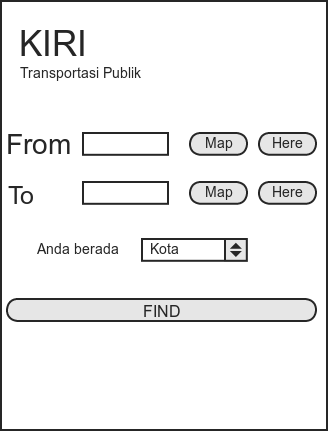
\includegraphics[scale=0.6]{Gambar/perancangan_antarmuka/Home}
	\caption{Antarmuka \textit{MainPage}}
	\label{fig:Antarmuka MainPage}
\end{figure}

\hspace{0.5cm} Antarmuka Kelas Map pada gambar ~\ref{fig:Antarmuka MainPage} merupakan tampilan awal saat aplikasi dijalankan. Antarmuka Kelas Map memiliki dua buah masukan, lima buah tombol, dan satu menu daftar. Berikut adalah detailnya.

Dua buah masukan yaitu.
\begin{itemize}
	\item Masukan lokasi asal\\
	Merupakan masukan lokasi asal mula pengguna ingin melakukan perjalanan.
	\item Masukan lokasi tujuan\\
	Merupakan masukan lokasi tujuan berhentinya perjalanan.
\end{itemize}

Lima buah tombol yaitu. 
\begin{itemize}
	\item Tombol map untuk lokasi asal\\
	Jika tombol ditekan maka akan berpindah ke kelas map untuk memilih lokasi asal di peta. Jika di kelas Map pengguna memilih lokasi maka pada masukan lokasi asal terdapat tulisan "Maps".
	\item Tombol here untuk lokasi asal\\
	Jika tombol ditekan maka lokasi asal adalah lokasi perangkat saat tombol ditekan dan masukan lokasi asal menjadi "here".
	\item Tombol map untuk lokasi tujuan\\
	Jika tombol ditekan maka akan berpindah ke kelas map untuk memilih lokasi tujuan di peta. Jika di kelas Map pengguna memilih lokasi maka pada masukan lokasi tujuan terdapat tulisan "Maps".
	\item Tombol here untuk lokasi tujuan\\
	Jika tombol ditekan maka lokasi tujuan adalah lokasi perangkat saat tombol ditekan dan masukan lokasi tujuan menjadi "here".
	\item Tombol find\\
	Jika tombol ditekan maka akan menampilkan daftar tempat asal dan tempat tujuan lalu mengarahkan ke Kelas Route.
\end{itemize}

Satu buah daftar yaitu.
\begin{itemize}
	\item Daftar kota yang tersedia\\
	Merupkan daftar kota yang tersedia (kota yang rute angkutan umumnya dapat ditemukan dengan aplikasi ini). Disaat aplikasi dijalankan maka daftar akan menunjuk ke kota terdekat tempat perangkat berada.
\end{itemize}

%Antarmuka list Tempat
\begin{figure}[h]
	\centering
		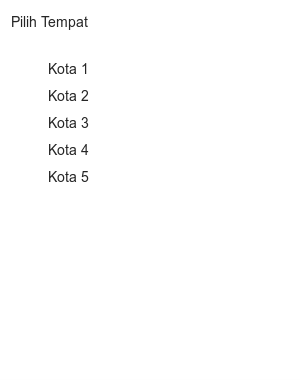
\includegraphics[scale=0.6]{Gambar/perancangan_antarmuka/ListTempat}
	\caption{Antarmuka Daftar Tempat}
	\label{fig:Antarmuka Daftar Tempat}
\end{figure}

\hspace{0.5cm} Antarmuka Daftar Tempat pada gambar ~\ref{fig:Antarmuka Daftar Tempat} merupakan daftar yang akan dimunculkan jika pengguna memasukan kata kunci pada pencarian tempat asal dan tempat tujuan. Daftar akan muncul jika didapat kembalian hasil pencarian lebih dari satu.

%Kelas Map
\subsection{Antarmuka Kelas \textit{Map}}
\label{lab:Antarmuka Kelas Map}

% Antarmuka Map
\begin{figure}[h]
	\centering
		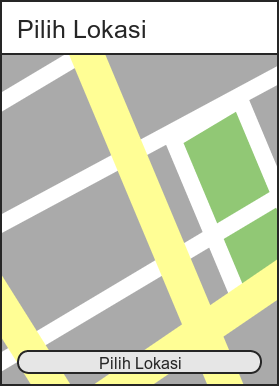
\includegraphics[scale=0.6]{Gambar/perancangan_antarmuka/Map}
	\caption{Antarmuka \textit{Map}}
	\label{fig:Antarmuka Map}
\end{figure}

\hspace{0.5cm} Antarmuka Kelas Map pada gambar ~\ref{fig:Antarmuka Map} merupakan antarmuka untuk menunjuk lokasi pada peta. Terdapat satu buah tombol yang akan dimunculkan jika pengguna sudah memilih lokasi. Jika tombol ditekan maka kordinat lokasi akan di simpan dan dikirim pada kelas MainPage dan halaman akan diarahkan ke kelas MainPage.

%Kelas Route
\subsection{Antarmuka Kelas \textit{Route}}
\label{lab:Antarmuka Kelas Route}

% Antarmuka route
\begin{figure}[h]
	\centering
		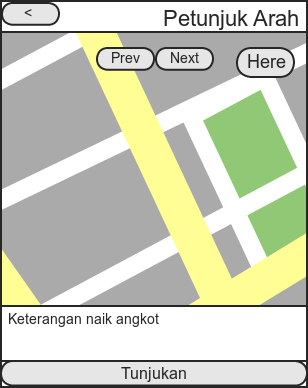
\includegraphics[scale=0.6]{Gambar/perancangan_antarmuka/Route}
	\caption{Antarmuka \textit{Route}}
	\label{fig:Antarmuka Route}
\end{figure}

\hspace{0.5cm} Antarmuka Kelas Route pada gambar ~\ref{fig:Antarmuka Route} merupakan antarmuka untuk melihat rute dari lokasi asal ke lokasi tujuan dalam bentuk daftar maupun peta. Terdapat empat buah tombol pada antarmuka Kelas Route. Berikut tombol yang terdapat pada Kelas Route. 
\begin{itemize}
	\item Tombol prev\\
	Jika tombol ditekan maka akan menunjuk titik sebelumnya pada rute peta.
	\item Tombol next\\
	Jika tombol ditekan maka akan menunjuk titik setelahnya pada rute peta.
	\item Tombol here\\
	Jika tombol ditekan maka akan menunjuk lokasi perangkat berada pada peta.
	\item Tombol Show List\\
	Jika tombol ditekan maka akan menunjuk atau menyembunyikan daftar rute.
\end{itemize}

% Antarmuka list route
\begin{figure}[h]
	\centering
		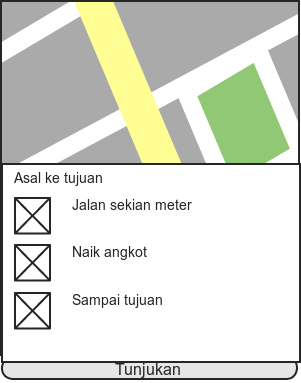
\includegraphics[scale=0.6]{Gambar/perancangan_antarmuka/ListRoute}
	\caption{Antarmuka Rute dalam bentuk Daftar}
	\label{fig:Antarmuka listRoute}
\end{figure}

\hspace{0.5cm} Antarmuka rute dalam bentuk daftar pada gambar ~\ref{fig:Antarmuka listRoute} merupakan antarmuka untuk melihat rute secara lebih jelas dengan keterangan tahap demi tahap disertai jarak dan waktu perjalanan. Antarmuka daftar dapat dilihat atau disembunyikan sesuai keinginan pengguna namun saat kelas Rute dibuka antarmuka daftar rute akan disembunyikan.}{}
\ifdefstring{\vbabe}{1}{\chapter{Implementasi dan Pengujian Aplikasi}
\label{chap:Implementasi dan Pengujian Aplikasi}

Pada bab 5 akan dibahas implementasi dan pengujian aplikasi pencari rute kendaraan umum untuk Windows Phone.

%Implementasi
\section{Implementasi}
\label{lab:Implementasi}
\hspace{0.5cm} Pada sub bab ini akan dijelaskan mengenai ligkungan yang digunakan untuk membangun aplikasi Pencari Rute Kendaraan Umum untuk Windows Phone. Pada lingkungan yang akan dibahas juga penulis membangun aplikasi sesuai rancangan yang telah dibahas pada bab 4 dan mengujinya.

%Perangkat Keras untuk Implementasi
\subsection{Perangkat Keras untuk Implementasi}
\label{lab:Perangkat Keras untuk Implementasi}
\hspace{0.5cm} Dalam membangun aplikasi ini perangkat keras yang digunakan adalah sebagai berikut:
\begin{enumerate}
	\item Komputer
		\begin{enumerate}
			\item Processor: intel Core i7-2620M CPU 2,7 GHz
			\item RAM: 4 GB
			\item Hardisk: 640 GB
			\item VGA: Intel HD 3000
		\end{enumerate}
		
	\item Perangkat Bergerak
		\begin{enumerate}
			\item Processor: 1,2 GHz
			\item RAM: 1 GB
			\item ROM: 8 GB
			\item Layar: 720 x 1280 pixel, 4,7 inch
			\item GPS
			\item Sensor: kompas, \textit{accelerometer}
		\end{enumerate}
\end{enumerate}

%Perangkat Lunak untuk Implementasi
\subsection{Perangkat Lunak untuk Implementasi}
\label{lab:Perangkat Lunak untuk Implementasi}
\hspace{0.5cm} Dalam membangun aplikasi ini perangkat lunak yang digunakan adalah sebagai berikut:
\begin{enumerate}
	\item Komputer
		\begin{enumerate}
			\item Sistem Operasi Windows 8.1
			\item IDE Visual Studio Express 2012
			\item Bahasa Pemrograman C\#
			\item Library .Net Framework 4.5
		\end{enumerate}
		
	\item Perangkat Bergerak
		\begin{enumerate}
			\item Sistem Operasi Windows Phone 8.1
		\end{enumerate}
\end{enumerate}

%Hasil Implementasi
\subsection{Hasil Implementasi}
\label{lab:Hasil Implementasi}
\hspace{0.5cm} Hasil implementasi dari perangkat lunak ini terbagi dalam tiga bagian, yaitu:
\begin{enumerate}
	\item Kode Program \\
	Kode Program pada perangkat lunak ditulis dengan menggunakan bahasa c\#. Bahasa C\# dipilih berdasarkan analisa pada bab 3 dan kemampuan penulis.
	\item Hasil kompilasi program \\
	Hasil dari kompilasi program berupa \textit{file} Kiri\_Debug\_AnyCPU.xap. \textit{File} ini dapat dipasang pada perangkat dengan sistem operasi Windows Phone versi 8 atau lebih tinggi.
	\item Antarmuka Aplikasi \\
	Berikut merupakan hasil implementasi antarmuka aplikasi Pencari Rute Kendaraan Umum untuk Windows phone.
\end{enumerate}

% Gambar antarmuka kelas MainPage
	\begin{figure}[!h]
		\centering
			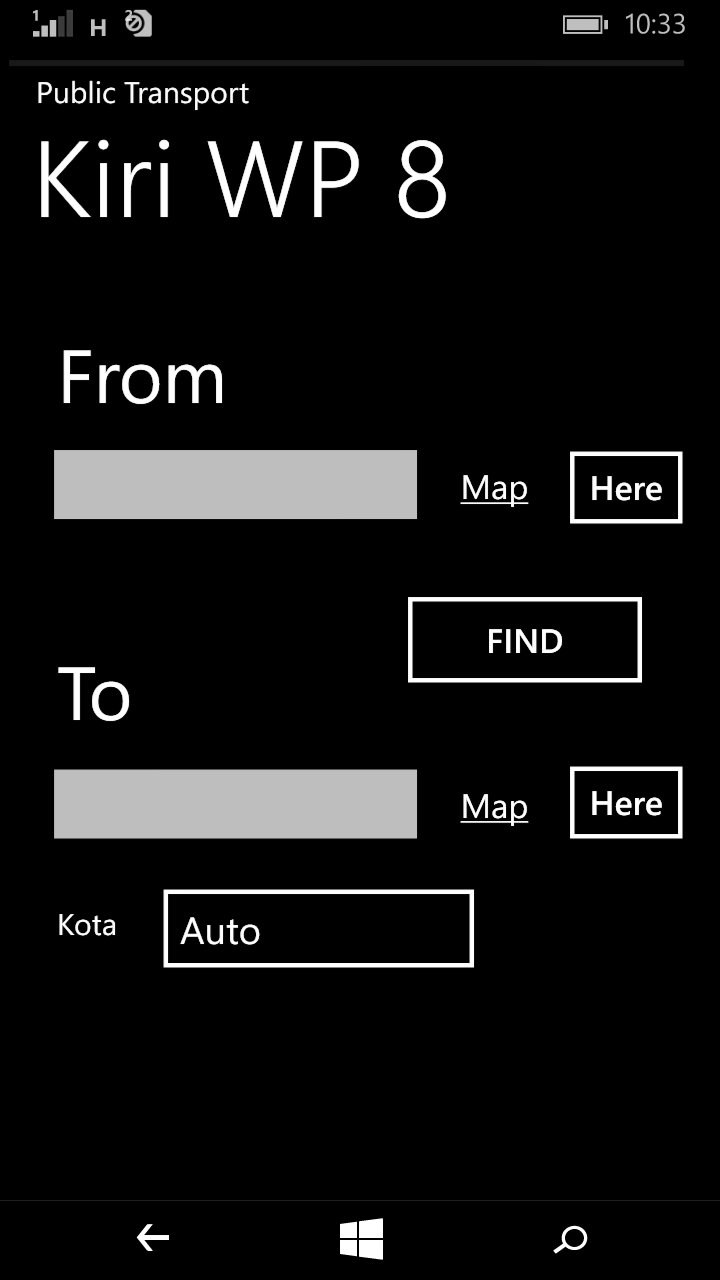
\includegraphics[scale=0.2]{Gambar/antarmuka/home}
		\caption{Gambar antarmuka kelas MainPage}
		\label{fig:antarmuka MainPage}
	\end{figure}
	
	\newpage
	
	% Gambar antarmuka Splash MainPage
	\begin{figure}[!h]
		\centering
			
\includegraphics[scale=0.2]{Gambar/antarmuka/splash}
		\caption{Gambar antarmuka Splash di kelas MainPage}
		\label{fig:antarmuka splash MainPage}
	\end{figure}	
	
	% Gambar antarmuka list di kelas MainPage
	\begin{figure}[!h]
		\centering
			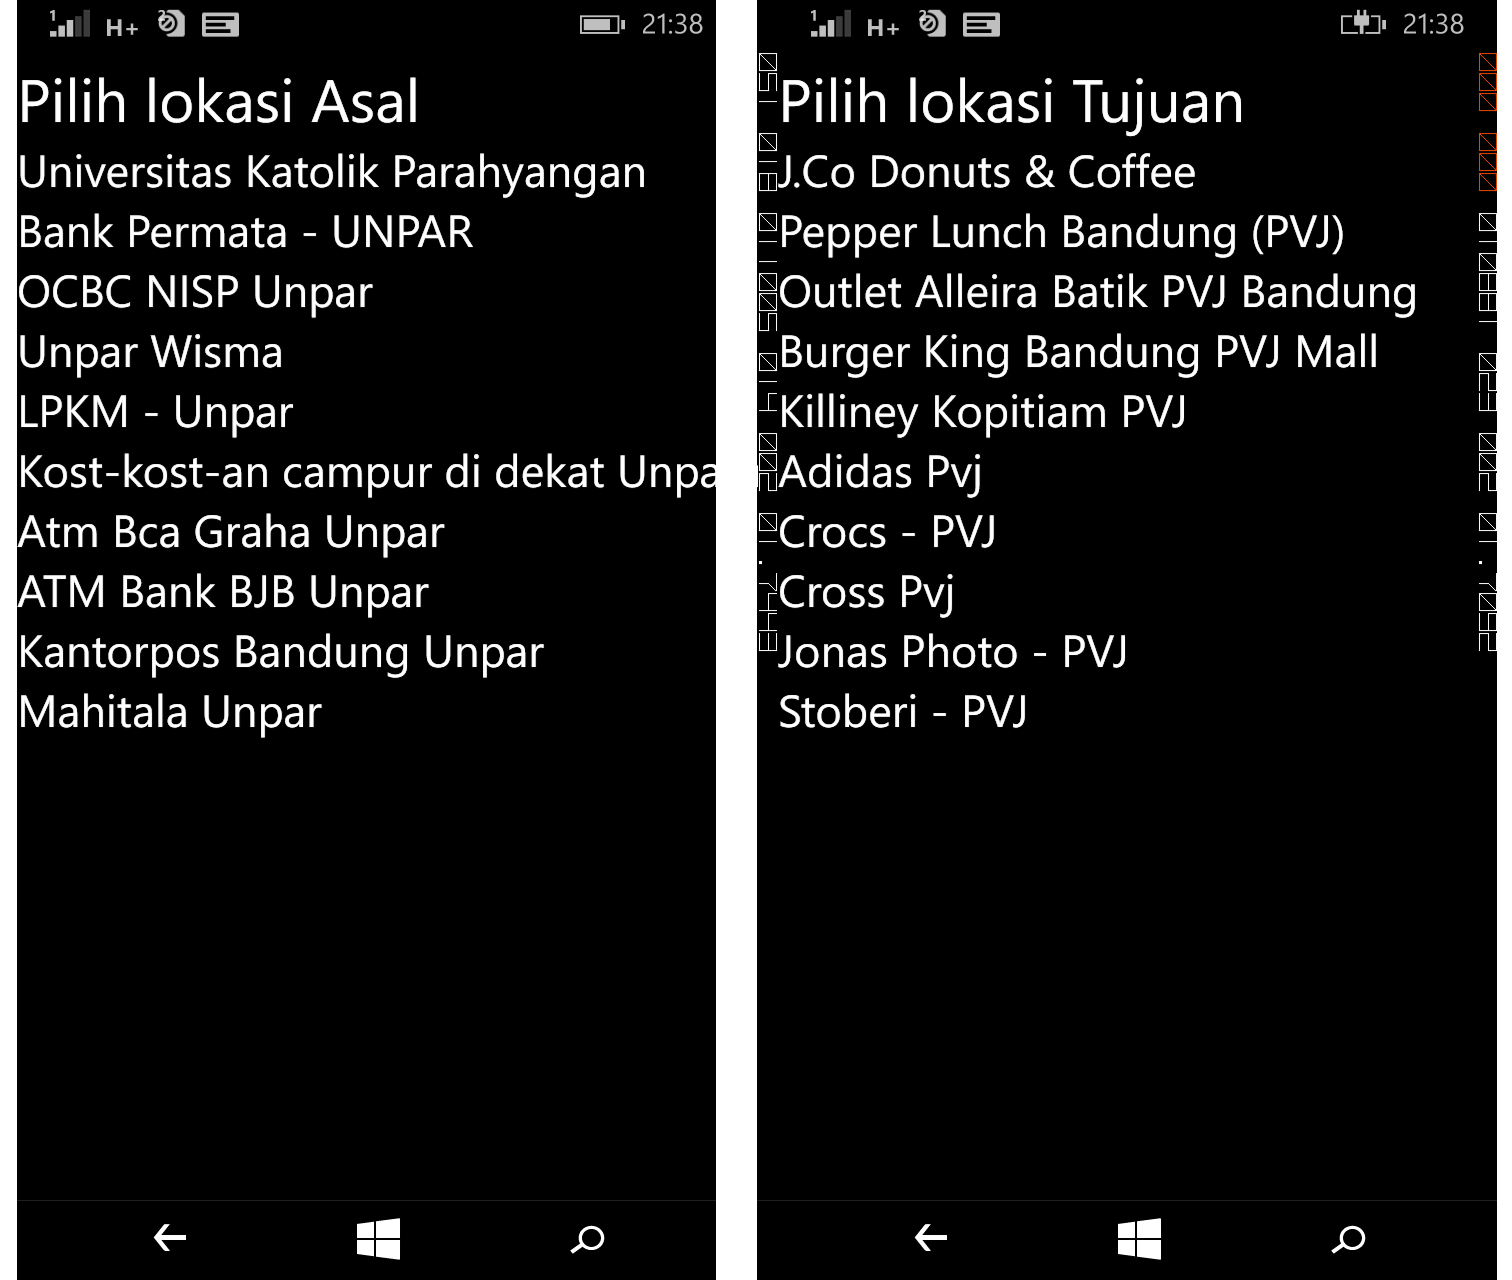
\includegraphics[scale=0.2]{Gambar/antarmuka/list_main}
		\caption{Gambar antarmuka \textit{list} asal dan \textit{list} tujuan di kelas MainPage}
		\label{fig:antarmuka list MainPage}
	\end{figure}
	
	% Gambar antarmuka kelas Map
	\begin{figure}[!h]
		\centering
			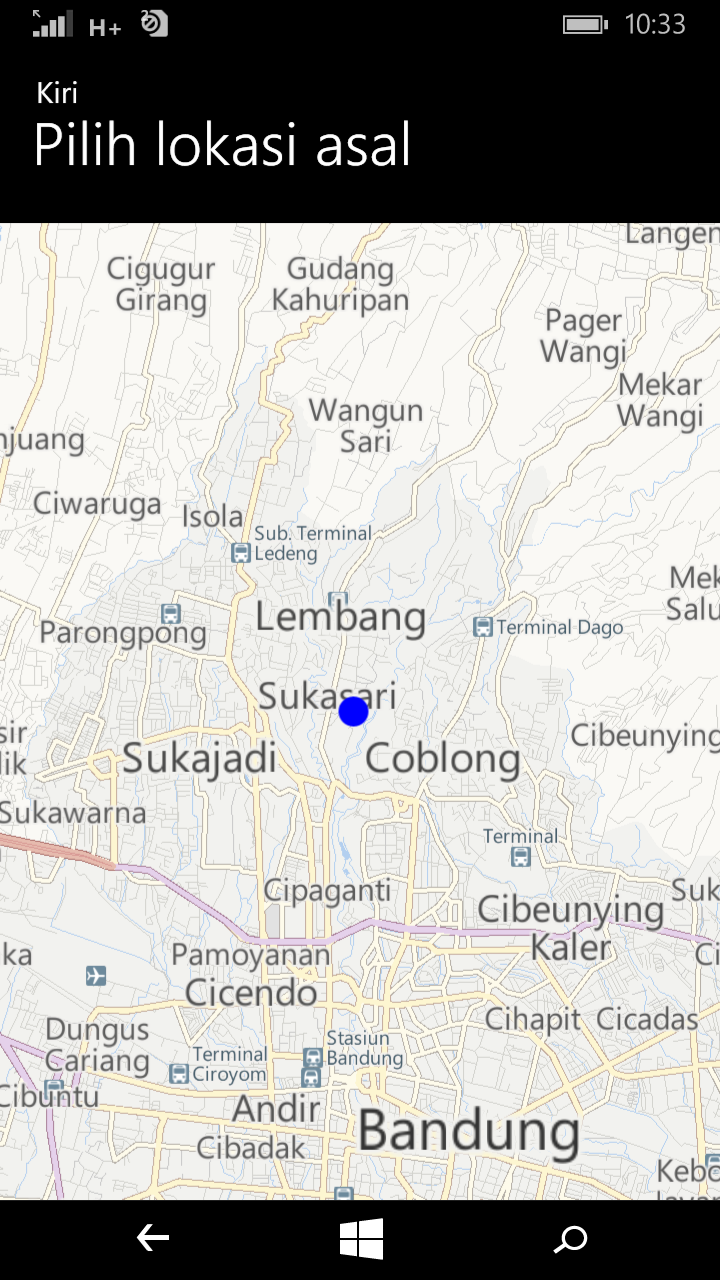
\includegraphics[scale=0.2]{Gambar/antarmuka/map}
		\caption{Gambar antarmuka kelas Map}
		\label{fig:antarmuka Map}
	\end{figure}
	
	% Gambar antarmuka menunggu di kelas Route
	\begin{figure}[!h]
		\centering
			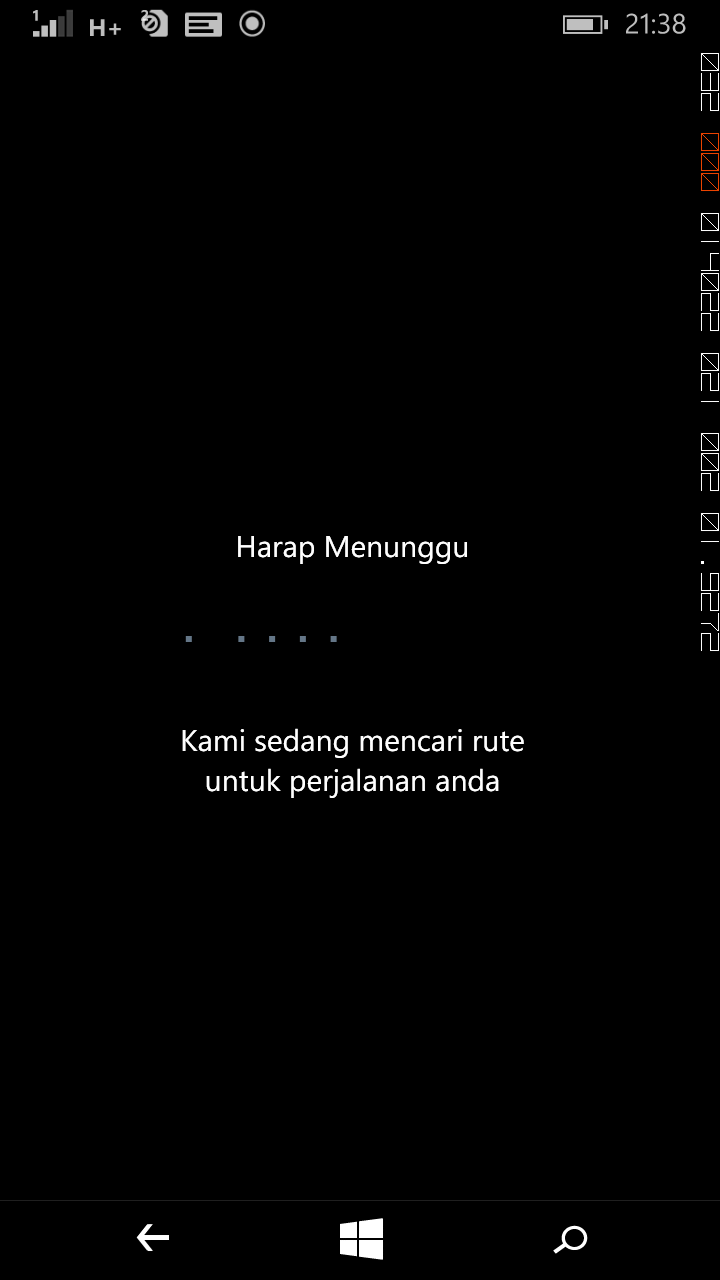
\includegraphics[scale=0.2]{Gambar/antarmuka/wait_route}
		\caption{Gambar antarmuka menunggu di kelas Route}
		\label{fig:antarmuka menunggu Route}
	\end{figure}
	
	% Gambar antarmuka kelas Route
	\begin{figure}[!h]
		\centering
			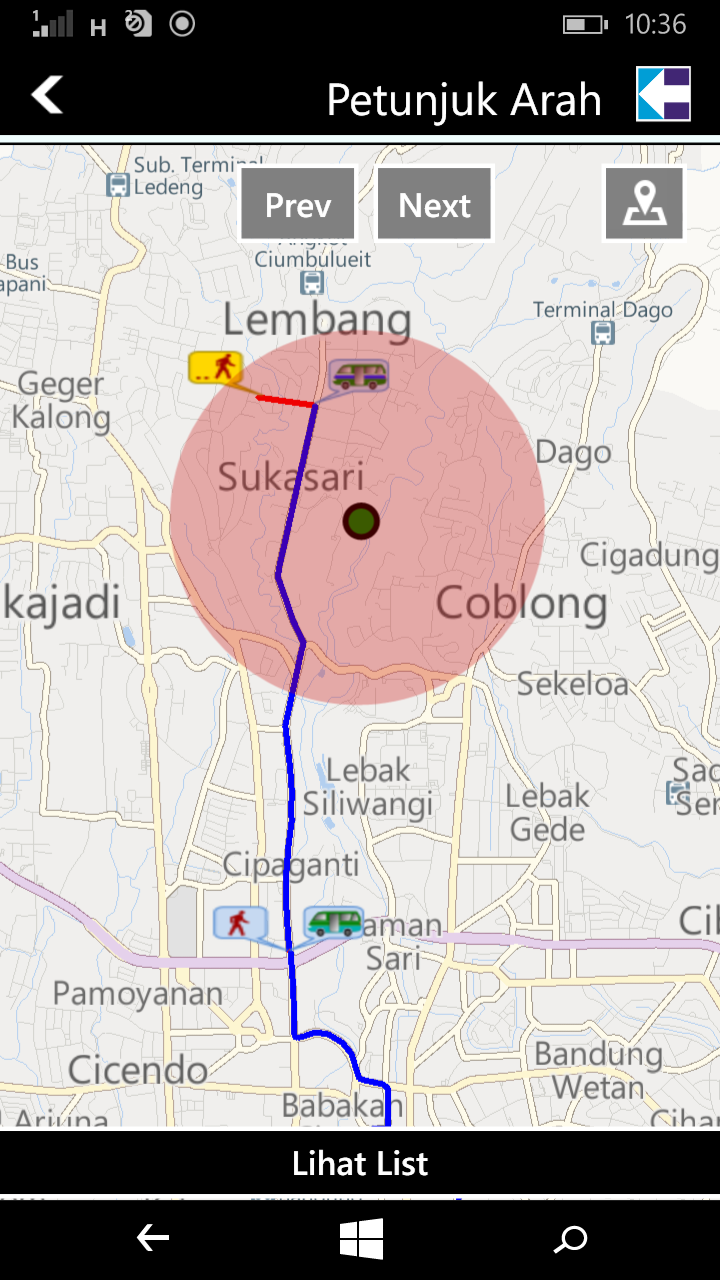
\includegraphics[scale=0.2]{Gambar/antarmuka/route_map}
		\caption{Gambar antarmuka kelas Route}
		\label{fig:antarmuka Route}
	\end{figure}
	
	% Gambar antarmuka kelas Route bentuk list
	\begin{figure}[!h]
		\centering
			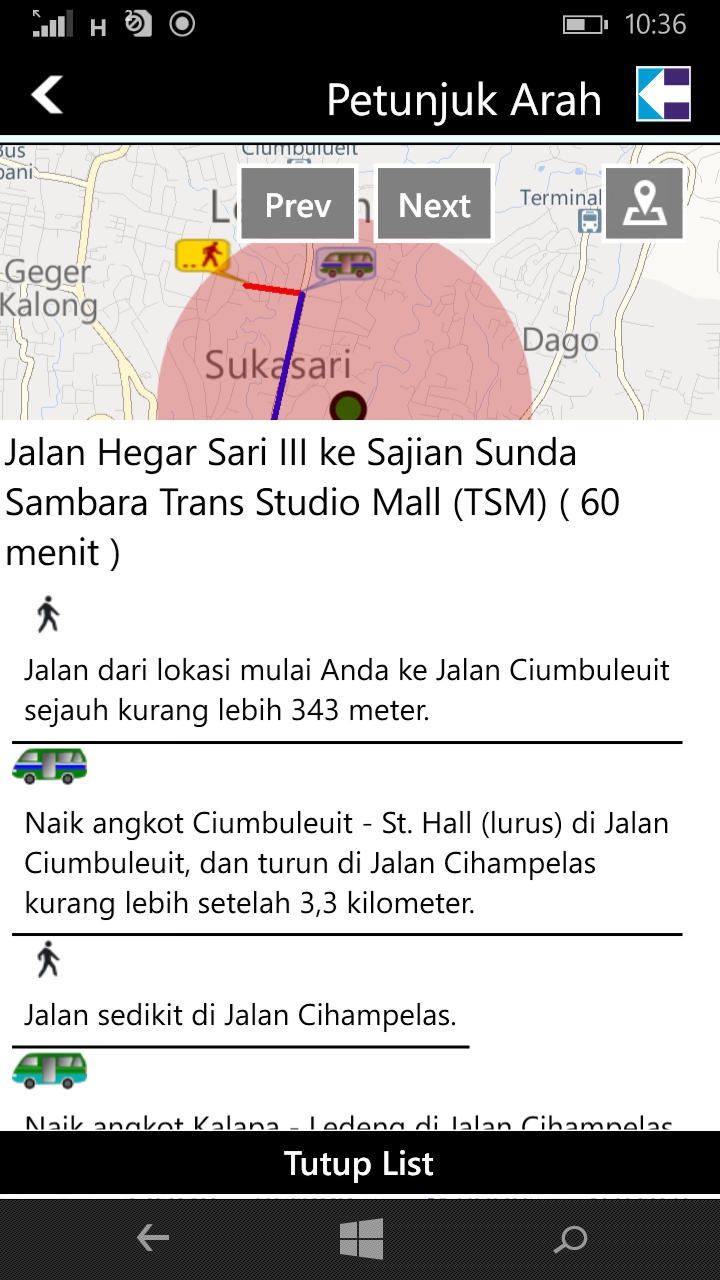
\includegraphics[scale=0.2]{Gambar/antarmuka/list_route}
		\caption{Gambar antarmuka \textit{list} di kelas Route}
		\label{fig:antarmuka list Route}
	\end{figure}

\newpage

%Pengujian
\section{Pengujian}
\label{lab:Pengujian}
\hspace{0.5cm} Pada bagian ini akan dibahas mengenai hasil pengujian yang telah dilakukan terhadap aplikasi yang telah dibangun penulis. Pengujian yang dilakukan terdiri dari dua bagian yaitu pengujian fungsional dan pengujian eksperimental. Pengujian fungsional bertujuan untuk memastikan semua fungsi aplikasi berjalan sesuai harapan. Sementara pengujian eksperimental bertujuan untuk mengetahui keberhasilan proses kerja dari aplikasi.

%Lingkungan Pengujian
\subsection{Lingkungan Pengujian}
\label{lab:Lingkungan Pengujian}
\hspace{0.5cm} Dalam proses pengujian perangkat lunak penulis menggunakan sistem operasi Windows Phone 8.1 dengan spesifikasi perangkat keras sebagai berikut.
\begin{enumerate}
	\item \textit{Processor} : 1.2 Ghz Quad Core
	\item RAM : 1 GB
	\item Layar : 1280 x 720 \textit{pixels}, 4,7 inch
	\item GPS : A-GPS, GLONASS, Beidou
\end{enumerate}

%Pengujian Fungsional untuk mengetahui kesesuaian reaksi nyata dengan yang diharapkan
\subsection{Pengujian Fungsional}
\label{lab:Pengujian Fungsional}
\hspace{0.5cm} Pengujian fungsional dilakukan untuk menguji kesesuaian reaksi yang terjadi dengan reaksi yang diharapkan. Untuk menguji kesesuaian rreaksi yang terjadi dengan reaksi yang diharapkan penulis menguji 5 orang pengguna dengan perintah sebagai berikut. 
\begin{enumerate}
	\item Carilah rute dari sini ke BIP!
	\item Carilah rute dari BIP ke Ciwalk!
	\item Carilah rute dari sini ke ITB pintu jalan Ganesa!
\end{enumerate}

Dari tiga perintah berikut penulis mengharapkan hasil sebagi berikut.
\begin{table}[h]
	\centering
		\begin{tabular}{|p{2cm}|p{10cm}|}\hline
				Perintah & Aksi Pengguna \\ \hline
				1 & Menekan tombol "Here" dan menulis kata "bip" pada TextBox \\ \hline
				2 & Menulis kata "bip" pada TextBox dan menulis kata "Ciwalk" pada TextBox \\ \hline
				3 & Menekan tombol "Here" dan menunjuk pintu masuk ITB yang di jalan Ganesa \\ \hline
		\end{tabular}
	\caption{Tabel hasil yang diharapkan penulis}
	\label{tab:TabelHasilyangdiharapkanPenulis}
\end{table}

Dari tiga perintah berikut didapat hasil sebagi berikut.
\begin{table}[h!]
	\centering
		\begin{tabular}{|p{1,5cm}|p{9cm}|p{2cm}|}\hline
				Perintah & Aksi Pengguna & Kesesuaian \\ \hline
				1 & Menekan tombol "Here" dan menulis "BIP" pada TextBox & sesuai \\ \hline
				2 & Menulis "BIP" pada TextBox dan menulis "CIwalk" pada TextBox & sesuai \\ \hline
				3 & Menekan tombol "Here" dan menulis "jl Ganesa" pada TextBox & tidak sesuai \\ \hline
		\end{tabular}
	\caption{Tabel hasil pengujian fungsionalitas terhadap pengguna 1}
	\label{tab:TabelHasilPengujianFungsionalitasTerhadapPengguna}
\end{table}

\begin{table}[h!]
	\centering
		\begin{tabular}{|p{1,5cm}|p{9cm}|p{2cm}|}\hline
				Perintah & Aksi Pengguna & Kesesuaian \\ \hline
				1 & Menekan tombol "Here" dan menulis "BIP" pada TextBox & sesuai \\ \hline
				2 & Menulis "BIP" pada TextBox dan menulis "CIwalk" pada TextBox & sesuai \\ \hline
				3 & Menekan tombol "Here" dan menunjuk pada peta & sesuai \\ \hline
		\end{tabular}
	\caption{Tabel hasil pengujian fungsionalitas terhadap pengguna 2}
	\label{tab:TabelHasilPengujianFungsionalitasTerhadapPengguna}
\end{table}

\newpage

\begin{table}[h!]
	\centering
		\begin{tabular}{|p{1,5cm}|p{9cm}|p{2cm}|}\hline
				Perintah & Aksi Pengguna & Kesesuaian \\ \hline
				1 & Menekan tombol "Here" dan menulis "BIP" pada TextBox & sesuai \\ \hline
				2 & Menulis "BIP" pada TextBox dan menulis "CIwalk" pada TextBox & sesuai \\ \hline
				3 & Menekan tombol "Here" dan menulis "ITB Ganeca" pada TextBox lalu menyadari tombol map dan menggunakannya & sesuai \\ \hline
		\end{tabular}
	\caption{Tabel hasil pengujian fungsionalitas terhadap pengguna 3}
	\label{tab:TabelHasilPengujianFungsionalitasTerhadapPengguna}
\end{table}

\begin{table}[h!]
	\centering
		\begin{tabular}{|p{1,5cm}|p{9cm}|p{2cm}|}\hline
				Perintah & Aksi Pengguna & Kesesuaian \\ \hline
				1 & Menekan tombol "Here" dan menulis "BIP" pada TextBox & sesuai \\ \hline
				2 & Menulis "BIP" pada TextBox dan menulis "CIwalk" pada TextBox & sesuai \\ \hline
				3 & Menekan tombol "Here" dan menulis "Institut Teknologi Bandung" pada TextBox & tidak sesuai \\ \hline
		\end{tabular}
	\caption{Tabel hasil pengujian fungsionalitas terhadap pengguna 4}
	\label{tab:TabelHasilPengujianFungsionalitasTerhadapPengguna}
\end{table}

\begin{table}[h!]
	\centering
		\begin{tabular}{|p{1,5cm}|p{9cm}|p{2cm}|}\hline
				Perintah & Aksi Pengguna & Kesesuaian \\ \hline
				1 & Menekan tombol "Here" dan menulis "BIP" pada TextBox & sesuai \\ \hline
				2 & Menulis "BIP" pada TextBox dan menulis "Ciwalk" pada TextBox & sesuai \\ \hline
				3 & Menekan tombol "Here" dan menulis "jalan ganesa" pada TextBox & tidak sesuai \\ \hline
		\end{tabular}
	\caption{Tabel hasil pengujian fungsionalitas terhadap pengguna 5}
	\label{tab:TabelHasilPengujianFungsionalitasTerhadapPengguna}
\end{table}

\hspace{0.5cm} Hasil pengujian menunjukan untuk perintah 1 dan 2 semua pengguna dapat menyelesaikan perintah dengan aksi yang sesuai. Sedangkan untuk perintah ke 3 sebagian pengguna masih salah dalam melakukan aksi yang sesuai. Dari hasil pengujian terhadap pengguna dapat dilihat pengguna lebih memilih untuk mengetikan kata kunci karena hal tersebut adalah yang paling mudah untuk dilakukan. Pengguna cenderung memikirkan suatu lokasi, memikirkan kata kunci lalu menuliskannya pada textbox di aplikasi. Menuliskan pada textbox memang lebih mudah dilakukan tapi ada beberapa pencarian spesifik yang tidak dapat dilakukan dengan mengetikan kata kunci.   

Penulis juga mencoba melakukan pengujian fungsionalitas untuk menguji aksi dan reaksi dari aplikasi. Hasil pengujian tersebut ditunjukan pada tabel ~\ref{tab:TabelHasilPengujianFungsionalitas}.
\begin{table}[h!]
	\centering
		\begin{tabular}{|p{1cm}|p{4cm}|p{6cm}|p{3cm}|}\hline
				No & Aksi Pengguna & Reaksi yang Diharapkan & Reaksi Perangkat lunak \\ \hline
				1 & Menjalankan aplikasi & Aplikasi menampilkan SplashScreen selama beberapa saat dan tampilan awal halaman MainPage ditampilkan & sesuai \\ \hline
				2 & Memasukan lokasi asal dan lokasi tujuan dari \textit{textbox} & \textit{Textbox} terisi sesuai masukan & sesuai \\ \hline
				3 & Memasukan lokasi asal atau lokasi tujuan berdasarkan lokasi perangkat dengan menekan tombol "here" & \textit{Textbox} lokasi asal atau lokasi tujuan terisi "here" & sesuai \\ \hline
				4 & Menekan tombol "maps" untuk memilih lokasi pada peta & Pindah halaman ke kelas Map & sesuai \\ \hline
				5 & Menekan lokasi pada peta lalu menekan tombol "pilih lokasi" & Lokasi ditandai dan pengguna diarahkan kembali ke kelas Main Page & sesuai \\ \hline
				6 & Memilih kota & Kota berubah sesusai yang dipilih pengguna & sesuai \\ \hline
				7 & Menekan tombol "Find" & Bila lokasi diambil dari peta dan lokasi perangkat maka tidak akan tampil \textit{ListBox} dan antarmuka dialihkan ke kelas Route & sesuai \\ \hline
				8 & & Bila input masukan berupa kata kunci tempat maka akan tampil \textit{ListBox} untuk dipilih, lalu setelah dipilih antarmuka dialihkan ke kelas Route & sesuai \\ \hline
				9 & Bila \textit{ListBox} ditampilkan dan pengguna memilih & \textit{ListBox} akan tertutup & sesuai \\ \hline
				10 & Pada kelas Route pengguna menekan tombol "here" & Pusat peta akan diarahkan ke lokasi pengguna berada & sesuai \\ \hline
				11 & Pada kelas Route pengguna menekan tombol "Tunjukan Daftar" & Jika daftar tertutup maka daftar akan terbuka & sesuai \\ \hline
				12 & & Jika daftar terbuka maka daftar akan tertutup & sesuai \\ \hline
				13 & Pada kelas Route pengguna menekan tombol "Next" & Pusat peta akan diarahkan ke pergantian transportasi berikutnya sesua kembalian Kiri disertai keterangan & sesuai \\ \hline
		\end{tabular}
	\caption{Tabel Hasil pengujian fungsionalitas}
	\label{tab:TabelHasilPengujianFungsionalitas}
\end{table}

\begin{table}[h!]
	\centering
		\begin{tabular}{|p{1cm}|p{4cm}|p{6cm}|p{3cm}|}\hline
				No & Aksi Pengguna & Reaksi yang Diharapkan & Reaksi Perangkat lunak \\ \hline
				14 & Pada kelas Route pengguna menekan tombol "Prev" & Pusat peta akan diarahkan ke pergantian transportasi sebelumnya sesua kembalian Kiri disertai keterangan & sesuai \\ \hline
				15 & Pada kelas Route pengguna menekan tombol "windows" & Keadaan aplikasi menjadi \textit{dormant} & tidak sesuai \\ \hline
		\end{tabular}
	\caption{Tabel Hasil pengujian fungsionalitas}
	\label{tab:TabelHasilPengujianFungsionalitas}
\end{table}

\hspace{0.5cm} Pada pengujian keadaan aplikasi dari keadaan \textit{running} ke \textit{dormant} tidak terjadi. Pada saat aplikasi dalam keadaan \textit{running} dan pengguna menekan tombol "windows" seharusnya keadaan aplikasi berpindah dari keadaan \textit{running} ke \textit{dormant} tetapi keadaan aplikasi malah \textit{terminate}. Hal tersebut dikarenakan aplikasi yang penulis kembangkan masih dalam mode debug.

%Pengujian Eksperimental untuk mengetahui tingkat keberhasilan proses kerja aplikasi
\subsection{Pengujian Eksperimental}
\label{lab:Pengujian Eksperimental}
\hspace{0.5cm} Pengujian eksperimental dilakukan untuk mengetahui keberhasilan aplikasi yang dibangun penulis. Berikut pengujian eksperimental yang dilakukan penulis.

	Pengujian 1
		\begin{itemize}
			\item Tempat : Rumah(Jalan Kejaksaan menuju Unpar)
			\item Waktu : Pukul 9 pada tanggal 7 April 2014 
			\item Pengalaman : \\
			\hspace{0.5cm} Pada pengujian 1 penulis memasukan alamat di dalam rumah untuk menuju Unpar. Saat penulis memasukan kata Unpar muncul daftar tempat sesuai kata kunci "Unpar", lalu penulis memilih "Universitas Katolik Parahyangan". Saat rute ditampilkan ada ketidaktepatan lokasi yang ditunjukan untuk lokasi asal(rumah) sedangkan untuk lokasi tujuan(Unpar) ditunjukan dengan tepat. Katidaktepatan tersebut kira-kira seratus meter dan lokasi ditandai lingkaran merah dengan ukuran besar. Hal tersebut dikarenakan tempat tertutup yang membuat GPS tidak menunjukan lokasi yang akurat. Tapi saat pengujian penulis berusaha mengikuti titik naik angkutan umum.
			\hspace{0.5cm}Penulis mulai dengan mengikuti petunjuk berjalan kaki menuju Jalan Tamblong. Saat keluar rumah lingkaran merah disekitar lokasi perangkat mulai mengecil yang menandakan akurasi GPS semakin baik. Angkutan kota yang penulis naiki pertama kali adalah angkutan kota kalapa. Sambil berada di angkot penulis mengamati rute yang ditunjukan aplikasi sudah sesuai dengan rute angkutan kota dan penunjuk lokasi menunjukan pergerakan dengan akurat. Angkutan kota yang penulis naiki berhenti di stasiun lalu penulis turun dan menuju Jalan Kebon Jukut. Di jalan kebon jukut penulis naik angkutan kota Ciumbuleuit - St. Hall. Selama perjalanan petunjuk rute dan \textit{polyline} sudah tepat sesuai rute angkutan kota. Angkutan kota ke dua langsung mengantarkan penulis menuju Jalan Ciumbuleuit untuk selanjutnya penulis berjalan menuju Unpar. Ketika sampai di Unpar, kordinat lokasi pada peta juga menunjukan titik di Unpar dan memakan waktu 65 menit.
			\hspace{0.5cm}Untuk perjalanan pulang penulis memulai dengan mencari rute dari Unpar menuju ke rumah di jalan Kejaksaan dengan mencari di peta. Perjalanan penulis mulai dengan naik angkot Ciumbuleuit - St. Hall (lurus). Angkot Ciumbuleuit - St. Hall (lurus) penulis naiki dari jalan Ciumbuleuit sampai jalan Cihampelas. Penulis turun di jalan Cihampelas dan naik angkot Kalapa - Ledeng di jalan Cihampelas. Namun di jalan Wastukencana rute pada peta menunjukan rute menyusuri jalan Wastukencana lalu ke jalan Aceh, namun angkot malah berbelok ke jalan Riau lalu ke jalan Purnawarman lalu ke jalan Aceh. Rute yang benar yaitu rute angkot dan bukan pada peta. Dari jalan Aceh angkot menuju jalan Sumatera lalu ke jalan Tamblong. Perjalanan penulispun berakhir setelah sampai di rumah.
		\end{itemize}


\subsection{Perbandingan Aplikasi Pencari Rute di Android dengan Aplikasi Pencari Rute di Windows Phone}
\label{lab:Perbandingan}
\hspace{0.5cm} Aplikasi Pencari rute yang penulis buat dengan yang ada di Android memiliki beberapa perbedaan. Berikut perbedaan antara aplikasi pencari rute di Android dengan Windows Phone.

\begin{table}[h]
	\centering
		\begin{tabular}{|p{4cm}|p{4cm}|p{4cm}|}\hline
				Perbedaan & Android & Windows Phone \\ \hline
				Mendapatkan Lokasi & Memanfaatkan pemanggilan lokasi secara berulang-ulang dan akan mengunah lokasi dari yang kurang tepat menjadi lebih tepat. & Memanfaatkan pemanggilan sampai mendapat akurasi yang cukup tepat. \\ \hline
				Map  & Google Map & Windows Phone Map \\ \hline
				Navigasi antar halaman  & Pengiriman parameter berupa nilai "key" dan "value" & Pengiriman state objek \\ \hline
		\end{tabular}
	\caption{Tabel perbedaan}
	\label{tab:TabelPerbedaan}
\end{table}}{}
\ifdefstring{\vbabf}{1}{\chapter{Kesimpulan dan Saran}
\label{chap:Kesimpulan dan Saran}

%Kesimpulan
\section{Kesimpulan}
\label{lab:Kesimpulan}

%Saran
\section{Saran}
\label{lab:Saran}}{}

%\bibliographystyle{ieeetr}
%\bibliography{pustaka}

\begin{thebibliography}{1}

	\bibitem{MSDN} Microsoft  {\em Windows Phone Silverlight development } 2014 : \url{http://msdn.microsoft.com/library/windows/apps/ff402535.aspx}.
	
	\bibitem{Kiri} Kiri Team  {\em KIRI API v2 Documentation} 2014 : \url{https://bitbucket.org/projectkiri/kiri_api/wiki/KIRI\% 20API\% 20v2\% 20Documentation}.
	
  \bibitem{Manning} Manning, Paul  {\em Pro Windows Phone App Development} 2013: Apress.

	\bibitem{Szostak} Szostak, Tomasz  {\em Windows Phone 8 Application Development Essentials} 2013: PACKT.
	

\end{thebibliography}

\appendix
\apptoc

\tampillmp{\vlmp}
%\ifdefstring{\vlmpa}{1}{\chapter{Kode Program Kelas MainPage}
\label{app:A}

\singlespacing 

\begin{lstlisting} [language=C,basicstyle=\tiny,caption=MainPage.xaml.cs]
using System;
using System.Collections.Generic;
using System.Linq;
using System.Net;
using System.Windows;
using System.Windows.Controls;
using System.Windows.Navigation;
using Microsoft.Phone.Controls;
using Microsoft.Phone.Shell;
using Kiri.Resources;
using System.Net.Http;
using System.Threading.Tasks;
using System.Windows.Input;
using Windows.Devices.Geolocation;
using System.IO.IsolatedStorage;
using System.Windows.Media;
using System.IO;
using System.Runtime.Serialization.Json;
using System.Text;
using Newtonsoft.Json;

using System.Windows.Controls.Primitives;
using System.ComponentModel;
using System.Threading;

using System.Device.Location; 

namespace Kiri
{
    public partial class MainPage : PhoneApplicationPage
    {
        // Constructor
        private Protocol protocol;
        private LocationFinder lFinder;
        private HttpClient httpClient = new HttpClient();
        private City c;
        private String myCity;

        private BackgroundWorker backgroundWorker;
        public String test = "aaa";
        
        public MainPage()
        {
            InitializeComponent();
            this.lFinder = new LocationFinder();
            this.c = new City();
            this.cmbCurrFrom.ItemsSource = c.city;
            this.protocol = new Protocol();
            ShowSplash();
        }

        protected override void OnNavigatedTo(System.Windows.Navigation.NavigationEventArgs e)
        {
            base.OnNavigatedTo(e);
            if (PhoneApplicationService.Current.State.ContainsKey("location"))
            {
                this.lFinder = (LocationFinder)PhoneApplicationService.Current.State["location"];
                //this.lFinder = (LocationFinder)PhoneApplicationService.Current.State["location"];
                if (lFinder.coorLongFrom != 0.0)
                {
                    fromBox.Text = lFinder.coorLongFrom + "aaa";
                }
                if (lFinder.coorLongTo != 0.0)
                {
                    fromBox.Text = lFinder.coorLongTo + "";
                }
                
                //check form
                if (lFinder.coorLatFrom == 0.0 && lFinder.coorLongFrom == 0.0 && !lFinder.addressFrom.Equals("Maps") && !lFinder.addressFrom.Equals("Here"))
                {
                    fromBox.Text = lFinder.addressFrom;
                }
                else if (lFinder.coorLatFrom != 0.0 && lFinder.coorLongFrom != 0.0)
                {
                    if (lFinder.addressFrom.Equals("Here"))
                    {
                        fromBox.Text = "Here";
                    }
                    else
                    {
                        fromBox.Text = "Maps";
                    }
                }
                //System.Diagnostics.Debug.WriteLine("stuff");
                if (lFinder.coorLatTo == 0.0 && lFinder.coorLongTo == 0.0 && !lFinder.addressTo.Equals("Maps") && lFinder.addressTo.Equals("Here"))
                {
                    toBox.Text = lFinder.addressTo;
                }
                else if (lFinder.coorLatTo != 0.0 && lFinder.coorLongTo != 0.0)
                {
                    if (lFinder.addressTo.Equals("Here"))
                    {
                        toBox.Text = "Here";
                    }
                    else
                    {
                        toBox.Text = "Maps";
                    }
                }
            }
            string forMaps = "";
            if (NavigationContext.QueryString.TryGetValue("for", out forMaps)) ;
            if (forMaps!=null)
            {
                if (forMaps.Equals("from"))
                {
                    fromBox.Text = "Maps";
                    //lFinder.addressFrom = "Maps";
                }
                else
                {
                    toBox.Text = "Maps";
                    //lFinder.addressTo = "Maps";
                }
            }
        }

        protected override void OnNavigatedFrom(NavigationEventArgs e)
        {
            base.OnNavigatedFrom(e);
            PhoneApplicationService.Current.State["location"] = lFinder;
        }

        private void Application_Deactivated(object sender, DeactivatedEventArgs e){
            PhoneApplicationService.Current.State["location"] = lFinder;
        }

        private void Application_Activated(object sender, ActivatedEventArgs e) {
            //Console.WriteLine("Test");
            if (PhoneApplicationService.Current.State.ContainsKey("location"))
            {
                this.lFinder = (LocationFinder)PhoneApplicationService.Current.State["location"];
                this.findRoute();
                /*
                if (lFinder.coorLongFrom != 0.0)
                {
                    fromBox.Text = lFinder.coorLongFrom + "aaa";
                }
                if (lFinder.coorLongTo != 0.0)
                {
                    fromBox.Text = lFinder.coorLongTo + "";
                }
                 * */
            }
        }

        private async void startRoute(object sender, RoutedEventArgs e)
        {
            
            String queryFrom = fromBox.Text;
            String queryTo = toBox.Text;
            RootObjectSearchPlace from = null; //Untuk Asal
            RootObjectSearchPlace to = null; //Untuk Tujuan

            //Check form
            if (!queryFrom.Equals("") && !queryTo.Equals(""))
            {
                //Validate From
                Boolean routeStatus = true;
                progressFindPlace.IsIndeterminate = true;
                //Get place from query
                if ((!queryFrom.Equals("Here") || !queryFrom.Equals("Maps")) && (lFinder.coorLatFrom == 0.0 && lFinder.coorLongFrom == 0.0)) //Check get location from GPS
                {
                    //Reference zhttps://msdn.microsoft.com/en-us/library/hh191443.aspx
                    //Task<string> requestFromTask = httpClient.GetStringAsync(new Uri(protocol.getSearchPlace(queryFrom, myCity)));
                    //requestFrom = await requestFromTask;
                    //from = new RootObjectSearchPlace();
                    //from = JsonConvert.DeserializeObject<RootObjectSearchPlace>(requestFrom); //Mengubah String menjadi objek
                    from = await protocol.getRequestSearch(queryFrom, myCity); //Mengubah String menjadi objek
                    if (from.searchresult.Count() == 0)
                    {
                        MessageBox.Show("Pencarian untuk kata " + fromBox.Text + " tidak ditemukan");
                        routeStatus = false;
                    }
                }
                if ((!queryTo.Equals("Here") || !queryTo.Equals("Maps")) && (lFinder.coorLatTo == 0.0 && lFinder.coorLongTo == 0.0)) //Check get location from GPS
                {
                    //Task<string> requestToTask = httpClient.GetStringAsync(new Uri(protocol.getSearchPlace(queryTo, myCity)));
                    //requestTo = await requestToTask;
                    //to = new RootObjectSearchPlace();
                    //to = JsonConvert.DeserializeObject<RootObjectSearchPlace>(requestTo);//Mengubah String menjadi objek
                    to = await protocol.getRequestSearch(queryTo, myCity); //Mengubah String menjadi objek
                    if (to.searchresult.Count() == 0)
                    {
                        MessageBox.Show("Pencarian untuk kata " + toBox.Text + " tidak ditemukan");
                        routeStatus = false;
                    }
                }
                //Check Query
                if (routeStatus == true)
                {
                    if ((lFinder.coorLatFrom == 0.0 && lFinder.coorLongFrom == 0.0))
                    {
                        getListItem(from, "from"); //Show Listbox for location From
                    }
                    if ((lFinder.coorLatTo == 0.0 && lFinder.coorLongTo == 0.0))
                    {
                        getListItem(to, "to");  //Show Listbox for location To
                    }
                    this.findRoute();
                }
                progressFindPlace.IsIndeterminate = false;
            }
            else {
                MessageBox.Show("Harap melengkapi tempat asal dan tempat tujuan");
            }
        }

        private void changeMapFrom(object sender, RoutedEventArgs e)
        {
            NavigationService.Navigate(new Uri("/Map.xaml?fromMapFor=from", UriKind.Relative));
            //NavigationService.Navigate(new Uri("/Map.xaml?fromMapFor=from", UriKind.Relative));    
        }
        private void changeMapTo(object sender, RoutedEventArgs e)
        {
            NavigationService.Navigate(new Uri("/Map.xaml?fromMapFor=to", UriKind.Relative));    
        }

        private void getHereFrom(object sender, RoutedEventArgs e)
        {
            this.lFinder.setCoordinateHere("from");
            fromBox.Text = "Here";
            lFinder.addressFrom = "Here";
        }

        private void getHereTo(object sender, RoutedEventArgs e)
        {
            this.lFinder.setCoordinateHere("to");
            toBox.Text = "Here";
            lFinder.addressTo = "Here";
        }

        /* old reference: zhttps://msdn.microsoft.com/en-us/library/bb412179%28v=vs.110%29.aspx*/

        //zhttps://social.msdn.microsoft.com/forums/windowsapps/en-us/7db73c64-86f7-4c43-9fd4-faa03421ea21/popup-blocking-listbox-selection-changed
        private void getListItem(RootObjectSearchPlace request,String forRequest)
        {
            //ListBox listFrom = new ListBox();
            //ListBox listTo = new ListBox();
            Dispatcher.BeginInvoke(new Action(delegate
            {
                if (request.status.ToString().Equals("ok")) //check status
                {
                    if (request.searchresult.Count() == 1)
                    {
                        if (forRequest.Equals("from"))
                        {
                            String locFrom = request.searchresult[0].location.ToString();
                            string[] coordinate = locFrom.Split(',');
                            lFinder.coorLatFrom = Double.Parse(coordinate[0]);
                            lFinder.coorLongFrom = Double.Parse(coordinate[1]);
                        }
                        else
                        {
                            String locTo = request.searchresult[0].location.ToString();
                            string[] coordinate = locTo.Split(',');
                            lFinder.coorLatTo = Double.Parse(coordinate[0]);
                            lFinder.coorLongTo = Double.Parse(coordinate[1]);
                        }
                        this.findRoute();
                    }
                    else
                    {
                        //LayoutRoot.Children.Add(getListItem(requestFrom));
                        if (forRequest.Equals("from"))
                        {
                            for (int c = 0; c < request.searchresult.Count; c++)
                            {
                                listPlaceFrom.Items.Add(request.searchresult[c].placename);
                            }
                            panelFrom.Visibility = Visibility.Visible;
                            listPlaceFrom.DataContext = request.searchresult;
                            listPlaceFrom.SelectionChanged += ListBoxSelectedPlace;
                        }
                        else
                        {
                            panelTo.Visibility = Visibility.Visible;
                            for (int c = 0; c < request.searchresult.Count; c++)
                            {
                                listPlaceTo.Items.Add(request.searchresult[c].placename);
                            }
                            listPlaceTo.DataContext = request.searchresult;
                            listPlaceTo.SelectionChanged += ListBoxSelectedPlace;
                        }
                    }
                }
                else
                {
                    MessageBox.Show("Error!");
                }
            }));
        }

        private void ListBoxSelectedPlace(object sender, SelectionChangedEventArgs e)
        {
            if (panelFrom.Visibility.Equals(Visibility.Visible))
            { //Check visibility
                if (null != (sender as ListBox).SelectedItem)
                {
                    if ((sender as ListBox).SelectedIndex >= 0)
                    {
                        String locFrom = searchCoordinatePlace((List<Searchresult>)listPlaceFrom.DataContext, listPlaceFrom.SelectedItem.ToString());  //((sender as ListBox).SelectedItem as Searchresult).placename;
                        string[] coordinate = locFrom.Split(',');
                        lFinder.coorLatFrom = Double.Parse(coordinate[0]);
                        lFinder.coorLongFrom = Double.Parse(coordinate[1]);
                        lFinder.addressFrom = listPlaceFrom.SelectedItem.ToString();
                    }
                }
                panelFrom.Children.Clear();
                panelFrom.Visibility = Visibility.Collapsed;
                //panelTo.Visibility = Visibility.Visible;
            }
            else {
                if (null != (sender as ListBox).SelectedItem)
                {
                    if ((sender as ListBox).SelectedIndex >= 0)
                    {
                        String locTo = searchCoordinatePlace((List<Searchresult>)listPlaceTo.DataContext, listPlaceTo.SelectedItem.ToString()); //((sender as ListBox).SelectedItem as Searchresult).placename;
                        string[] coordinate = locTo.Split(',');
                        lFinder.coorLatTo = Double.Parse(coordinate[0]);
                        lFinder.coorLongTo = Double.Parse(coordinate[1]);
                        lFinder.addressTo = listPlaceTo.SelectedItem.ToString();
                    }
                }
                panelTo.Children.Clear();
                panelTo.Visibility = Visibility.Collapsed;
            }
            this.findRoute();
        }

        public string searchCoordinatePlace(List<Searchresult> listResult, string place) { //Pasti ketemu
            String coordinate = "0.0";
            for (int c = 0; c < listResult.Count; c++)
            {
                if (place.Equals(listResult[c].placename))
                {
                    coordinate = listResult[c].location;
                    c = listResult.Count;
                }
            }
            return coordinate;
        }

        public void findRoute()
        {
            if ((lFinder.coorLatFrom != 0.0 && lFinder.coorLongFrom != 0.0) && (lFinder.coorLatTo != 0.0 && lFinder.coorLongTo != 0.0))
            {
                NavigationService.Navigate(new Uri("/Route.xaml", UriKind.Relative)); //start=" + locationFrom + "&nameFrom=" + fromBox.Text + "&finish=" + locationTo + "&nameTo=" + toBox.Text
            }
        }

        private void changeCity(object sender, SelectionChangedEventArgs e)
        {
            if (!cmbCurrFrom.SelectedItem.Equals(null))
            {
                switch (cmbCurrFrom.SelectedItem.ToString())
                {
                    case "Bandung":
                        this.myCity="bdo";
                        break;
                    case "Jakarta":
                        this.myCity="cgk";
                        break;
                    case "Malang":
                        this.myCity="mlg";
                        break;
                    case "Surabaya":
                        this.myCity="sub";
                        break;     
                    default:
                        this.myCity="bdo"; //Finder Auto
                        break;
                }
            }
        }

        public void showCity() {
            int indexCity = -1;
            while (indexCity == -1)
            {
                indexCity = c.getNearby(lFinder.coorLat, lFinder.coorLong);
            }
            this.myCity = c.cityCode[indexCity];
        }

        private void ShowSplash()
        {
            this.popup.IsOpen = true;
            StartLoadingData();
        }

        private void StartLoadingData()
        {
            backgroundWorker = new BackgroundWorker();
            backgroundWorker.DoWork += new DoWorkEventHandler(backgroundWorker_DoWork);
            backgroundWorker.RunWorkerCompleted += new RunWorkerCompletedEventHandler(backgroundWorker_RunWorkerCompleted);
            backgroundWorker.RunWorkerAsync();
        }

        private void backgroundWorker_DoWork(object sender, DoWorkEventArgs e)
        {
            showCity();
        }

        private void backgroundWorker_RunWorkerCompleted(object sender, RunWorkerCompletedEventArgs e)
        {
            this.Dispatcher.BeginInvoke(() =>
            {
                this.cmbCurrFrom.SelectedIndex = c.getIndexFromCityCode(myCity);
                this.popup.IsOpen = false;
            });
        }
    }
}
\end{lstlisting}

\begin{lstlisting} [language=C,basicstyle=\tiny,caption=MainPage.xaml]
	<!--Logo kiri from kiri.travel 
    Icon from modernuiicons.com
    -->
    <phone:PhoneApplicationPage
    x:Class="Kiri.MainPage"
    xmlns="http://schemas.microsoft.com/winfx/2006/xaml/presentation"
    xmlns:x="http://schemas.microsoft.com/winfx/2006/xaml"
    xmlns:phone="clr-namespace:Microsoft.Phone.Controls;assembly=Microsoft.Phone"
    xmlns:shell="clr-namespace:Microsoft.Phone.Shell;assembly=Microsoft.Phone"
    xmlns:d="http://schemas.microsoft.com/expression/blend/2008"
    xmlns:mc="http://schemas.openxmlformats.org/markup-compatibility/2006"
    xmlns:toolkit="clr-namespace:Microsoft.Phone.Controls;assembly=Microsoft.Phone.Controls.Toolkit"
    mc:Ignorable="d"
    FontFamily="{StaticResource PhoneFontFamilyNormal}"
    FontSize="{StaticResource PhoneFontSizeNormal}"
    Foreground="{StaticResource PhoneForegroundBrush}"
    SupportedOrientations="Portrait" Orientation="Portrait"
    shell:SystemTray.IsVisible="True">

    <!--LayoutRoot is the root grid where all page content is placed-->
    <Grid x:Name="LayoutRoot" Background="Transparent" Margin="0,0,0,0">
        <Grid.RowDefinitions>
            <RowDefinition Height="158"/>
            <RowDefinition Height="3"/>
            <RowDefinition Height="*"/>
        </Grid.RowDefinitions>

        <!-- LOCALIZATION NOTE:
            To localize the displayed strings copy their values to appropriately named
            keys in the app's neutral language resource file (AppResources.resx) then
            replace the hard-coded text value between the attributes' quotation marks
            with the binding clause whose path points to that string name.

            For example:

                Text="{Binding Path=LocalizedResources.ApplicationTitle, Source={StaticResource LocalizedStrings}}"

            This binding points to the template's string resource named "ApplicationTitle".

            Adding supported languages in the Project Properties tab will create a
            new resx file per language that can carry the translated values of your
            UI strings. The binding in these examples will cause the value of the
            attributes to be drawn from the .resx file that matches the
            CurrentUICulture of the app at run time.
         -->

        <!--TitlePanel contains the name of the application and page title-->
        <StackPanel x:Name="TitlePanel" Grid.Row="0" Margin="6,10,6,0" RenderTransformOrigin="0.5,0.5" Height="108" VerticalAlignment="Top">
            <StackPanel.RenderTransform>
                <CompositeTransform SkewX="0.781" TranslateX="0.736"/>
            </StackPanel.RenderTransform>
            <TextBlock Text="Public Transport" Style="{StaticResource PhoneTextNormalStyle}" Margin="12,0"/>
            <TextBlock Text="Kiri WP 8" Margin="9,-7,0,0" Style="{StaticResource PhoneTextTitle1Style}" Height="111"/>
        </StackPanel>
        <Popup x:Name="popup" Margin="6,0,-6,10" Grid.RowSpan="3">
            <Grid Background="Black" Height="756" Width="484">
                <Image Source="/icons/kiri_logo.png" Margin="144,175,159,358" RenderTransformOrigin="1.509,0.516"/>
                <ProgressBar Height="34" Width="481" IsIndeterminate="True" Margin="-7,489,10,233"/>
            </Grid>
        </Popup>
        <!--ContentPanel - place additional content here-->
        <Grid x:Name="ContentPanel" Margin="0,0,0,0" Grid.Row="1" Grid.RowSpan="2">
            <TextBlock Text="From" Style="{StaticResource PhoneTextNormalStyle}" Margin="26,0,278,484" FontSize="50"/>
            <TextBlock Text="To" Style="{StaticResource PhoneTextNormalStyle}" Margin="26,137,361,274" FontSize="50"/>
            <TextBox x:Name="fromBox" HorizontalAlignment="Left" Margin="12,70,0,0" TextWrapping="Wrap" VerticalAlignment="Top" FontSize="24" Width="325" Height="76"/>
            <TextBox x:Name="toBox" HorizontalAlignment="Left" Margin="12,209,0,0" TextWrapping="Wrap" VerticalAlignment="Top" FontSize="24" Width="325" Height="76"/>
            <Button Content="FIND" HorizontalAlignment="Left" Margin="10,376,0,0" VerticalAlignment="Top" Click="startRoute" Height="81" Width="460"/>
            <Button HorizontalAlignment="Left" Margin="330,209,0,0" VerticalAlignment="Top" Click="changeMapTo" Height="77" Width="83">
                <Image Source="icons/map.png" Margin="-14 -12 0 0" Width="60" Height="60"></Image>
            </Button>
            <Button  HorizontalAlignment="Left" Margin="329,69,0,0" VerticalAlignment="Top" Click="changeMapFrom" Height="77" Width="83">
                <Image Source="icons/map.png" Margin="-14 -12 0 0" Width="60" Height="60"></Image>
            </Button>
            <Button HorizontalAlignment="Left" Margin="393,210,0,0" VerticalAlignment="Top" Click="getHereTo" Height="77" Width="83">
                <Image Source="icons/marker.png" Margin="-14 -12 0 0" Width="60" Height="60"></Image>
            </Button>
            <Button  HorizontalAlignment="Left" Margin="393,70,0,0" VerticalAlignment="Top" Click="getHereFrom" Height="77" Width="83">
                <Image Source="icons/marker.png" Margin="-14 -12 0 0" Width="60" Height="60"></Image>
            </Button>
            <TextBlock HorizontalAlignment="Left" Margin="20,315,0,0" TextWrapping="Wrap" Text="Anda berada di kota" VerticalAlignment="Top"/>
            <toolkit:ListPicker BorderThickness="0" ScrollViewer.VerticalScrollBarVisibility="Auto" Margin="217,298,74,-45" Name="cmbCurrFrom" SelectionChanged="changeCity" Visibility="Visible">
            </toolkit:ListPicker>
            <ProgressBar x:Name="progressFindPlace" Background="Black" HorizontalAlignment="Left" Height="19" Margin="0,-24,0,0" VerticalAlignment="Top" Width="456" RenderTransformOrigin="0.493,1.056"/>

            <StackPanel x:Name="panelFrom" HorizontalAlignment="Stretch"  Canvas.ZIndex="10" Margin="0,-150,0,5" VerticalAlignment="Stretch" Visibility="Collapsed" Background="Black">
                <TextBlock x:Name="textFrom" TextWrapping="Wrap" Text="Pilih lokasi Asal" FontSize="40"/>
                <ListBox x:Name="listPlaceFrom" Padding="10" Height="700" FontSize="30"></ListBox>
            </StackPanel>
            <StackPanel x:Name="panelTo" HorizontalAlignment="Stretch"  Canvas.ZIndex="5" Margin="0,-150,0,5" VerticalAlignment="Stretch"  Visibility="Collapsed" Background="Black" Grid.ColumnSpan="2">
                <TextBlock x:Name="textTo" TextWrapping="Wrap" Text="Pilih lokasi Tujuan" FontSize="40"/>
                <ListBox x:Name="listPlaceTo" Padding="10" Height="700" FontSize="30" ></ListBox>
            </StackPanel>
        </Grid>



        <!--Uncomment to see an alignment grid to help ensure your controls are
            aligned on common boundaries.  The image has a top margin of -32px to
            account for the System Tray. Set this to 0 (or remove the margin altogether)
            if the System Tray is hidden.

            Before shipping remove this XAML and the image itself.-->
        <!--<Image Source="/Assets/AlignmentGrid.png" VerticalAlignment="Top" Height="800" Width="480" Margin="0,-32,0,0" Grid.Row="0" Grid.RowSpan="2" IsHitTestVisible="False" />-->
    </Grid>

</phone:PhoneApplicationPage>
\end{lstlisting}}{}
%\ifdefstring{\vlmpb}{1}{\chapter{The Source Code}
\label{app:B}

%selalu gunakan single spacing untuk source code !!!!!
\singlespacing 
% language: bahasa dari kode program
% terdapat beberapa pilihan : Java, C, C++, PHP, Matlab, R, dll
%
% basicstyle : ukuran font untuk kode program
% terdapat beberapa pilihan : tiny, scriptsize, footnotesize, dll
%
% caption : nama yang akan ditampilkan di dokumen akhir, lihat contoh
\begin{lstlisting}[language=Java,basicstyle=\tiny,caption=MyFurSet.java]

import java.util.ArrayList;
import java.util.Collections;
import java.util.HashSet;

/**
 *
 * @author Lionov
 */

//class for set of vertices close to furthest edge
public class MyFurSet {
    protected int id;                                  //id of the set
    protected MyEdge FurthestEdge;                     //the furthest edge
    protected HashSet<MyVertex> set;                   //set of vertices close to furthest edge
    protected ArrayList<ArrayList<Integer>> ordered;   //list of all vertices in the set for each trajectory
    protected ArrayList<Integer> closeID;              //store the ID of all vertices
    protected ArrayList<Double> closeDist;             //store the distance of all vertices
    protected int totaltrj;                            //total trajectories in the set

    /**
     * Constructor
     * @param id : id of the set
     * @param totaltrj : total number of trajectories in the set
     * @param FurthestEdge : the furthest edge
     */
    public MyFurSet(int id,int totaltrj,MyEdge FurthestEdge) {
        this.id = id;
        this.totaltrj = totaltrj;
        this.FurthestEdge = FurthestEdge;
        set = new HashSet<MyVertex>();
        ordered = new ArrayList<ArrayList<Integer>>();
        for (int i=0;i<totaltrj;i++) ordered.add(new ArrayList<Integer>());
        closeID = new ArrayList<Integer>(totaltrj);
        closeDist = new ArrayList<Double>(totaltrj);
        for (int i = 0;i <totaltrj;i++) {
            closeID.add(-1);
            closeDist.add(Double.MAX_VALUE);
        }
    }

    /**
     * set a vertex into the set
     * @param v : vertex to be added to the set
     */
    public void add(MyVertex v) {
        set.add(v);
    }

    /**
     * check whether vertex v is a member of the set
     * @param v : vertex to be checked
     * @return true if v is a member of the set, false otherwise
     */
    public boolean contains(MyVertex v) {
        return this.set.contains(v);
    }
}
\end{lstlisting}}{}
%\ifdefstring{\vlmpc}{1}{\chapter{Kode Program kelas Route}
\label{app:C}

%selalu gunakan single spacing untuk source code !!!!!
\singlespacing 
% language: bahasa dari kode program
% terdapat beberapa pilihan : Java, C, C++, PHP, Matlab, R, dll
%
% basicstyle : ukuran font untuk kode program
% terdapat beberapa pilihan : tiny, scriptsize, footnotesize, dll
%
% caption : nama yang akan ditampilkan di dokumen akhir, lihat contoh

\begin{lstlisting} [language=C,basicstyle=\tiny,caption=Route.xaml.cs]
using System;
using System.Collections.Generic;
using System.Linq;
using System.Net;
using System.Windows;
using System.Windows.Controls;
using System.Windows.Navigation;
using Microsoft.Phone.Controls;
using Microsoft.Phone.Shell;

using System.Device.Location; // Provides the GeoCoordinate class.
using Windows.Devices.Geolocation; //Provides the Geocoordinate class.
using System.Windows.Media;
using System.Windows.Shapes;
using Microsoft.Phone.Maps.Controls;
using Microsoft.Phone.Maps.Toolkit;

using System.Threading.Tasks;
using System.Net.Http;
using System.IO;
using System.Runtime.Serialization.Json;
using System.Text;
using Newtonsoft.Json;
using System.Windows.Media.Imaging;
using System.ComponentModel;
using System.Windows.Controls.Primitives;
using System.Threading;
using System.IO.IsolatedStorage;
using System.Windows.Threading;
using System.Diagnostics;

namespace Kiri
{
    public partial class Route : PhoneApplicationPage
    {
        private Boolean listBoxStatus; //true == show, false == hide
        private LocationFinder lFinder;
        private Point[] arrayFocus;
        private String[] detailRoute;
        private int focusPointNumber;
        private MapLayer routeLayer;
        private MapLayer myLocationLayer;
        private Protocol p;
        private Boolean routeReady;

        private Geolocator geolocator = null;
        private BackgroundWorker backgroundWorker;
        private DispatcherTimer newTimer;
        private Boolean timeOut = false;

        public Route()
        {
            InitializeComponent();
            this.lFinder = null;
            this.arrayFocus = null;
            this.detailRoute = null;
            this.focusPointNumber = 0;
            this.routeLayer = new MapLayer();
            this.myLocationLayer = new MapLayer();
            this.p = new Protocol();
            this.routeReady = false;
            this.newTimer = new DispatcherTimer();
            newTimer.Interval = new TimeSpan(0, 0, 60);
            newTimer.Tick += OnTimerTick;
            newTimer.Start();

            ShowLoading();
        }

        protected override void OnNavigatedTo(System.Windows.Navigation.NavigationEventArgs e)
        {
            base.OnNavigatedTo(e);
            if (PhoneApplicationService.Current.State.ContainsKey("location"))
            {
                this.lFinder = (LocationFinder)PhoneApplicationService.Current.State["location"];
            }
            this.TrackLocation();

            //detect location
            if (IsolatedStorageSettings.ApplicationSettings.Contains("LocationConsent"))
            {
                return;
            }
        }

        protected override void OnNavigatedFrom(NavigationEventArgs e)
        {
            base.OnNavigatedFrom(e);
        }

        private void Application_Deactivated(object sender, DeactivatedEventArgs e)
        {
            PhoneApplicationService.Current.State["location"] = lFinder;
        }

        private void TrackLocation()
        {
            geolocator = lFinder.geolocator;

            geolocator.StatusChanged += geolocator_StatusChanged;
            geolocator.PositionChanged += geolocator_PositionChanged;
        }

        void geolocator_PositionChanged(Geolocator sender, PositionChangedEventArgs args)
        {
            Dispatcher.BeginInvoke(() =>
            {
                drawMyLocationOnTheMap(args.Position.Coordinate.Latitude, args.Position.Coordinate.Longitude);
                lFinder.setPositionChanged(sender,args);
            });
        }

        public async void Find()
        {
            Boolean status = true; 
            HttpClient httpClient = new HttpClient();

            RootObjectFindRoute r = await p.getRequestRoute(lFinder.coorLatFrom, lFinder.coorLongFrom, lFinder.coorLatTo, lFinder.coorLongTo);
            if (r.status.Equals("ok"))
            {
                if (!r.routingresults[0].steps[0][3].Equals("Maaf, kami tidak dapat menemukan rute transportasi publik untuk perjalanan Anda.")) //Check ditemukan atau tidak
                {
                    this.setRouteToMap(r);
                }
                else {
                    MessageBox.Show("Maaf, kami tidak dapat menemukan rute transportasi publik untuk perjalanan Anda.");
                    status = false; 
                }
            }
            else {
                MessageBox.Show("Error");
                status = false; 
            }

            if (status == false)
            {
                this.lFinder.reset();
								PhoneApplicationService.Current.State["location"] = lFinder;
                NavigationService.Navigate(new Uri("/MainPage.xaml", UriKind.Relative));
            }
        }

        private void setRouteToMap(RootObjectFindRoute r) {
            MapPolyline routeRoad = new MapPolyline();
            for (int i = 0; i < 1; i++) // Ambil Routing result yg pertama
            {
                this.arrayFocus = new Point[r.routingresults[i].steps.Count + 1];
                this.detailRoute = new String[r.routingresults[i].steps.Count + 1];
                for (int j = 0; j < r.routingresults[i].steps.Count; j++)
                {
                    routeRoad = new MapPolyline();
                    if (r.routingresults[i].steps[j][0].ToString().Equals("walk"))
                    {
                        routeRoad.StrokeColor = Color.FromArgb(255, 255, 0, 0);
                    }
                    else
                    {
                        routeRoad.StrokeColor = Color.FromArgb(255, 0, 0, 255);
                    }
                    routeRoad.StrokeThickness = 4;
                    GeoCoordinate geoCoo = new GeoCoordinate();
                    //Trim character
                    String temp = r.routingresults[i].steps[j][2].ToString();
                    char[] charsToTrim = { '[', ']', ' ' };
                    String result = temp.Trim(charsToTrim);
                    result = result.Replace("\"", "");
                    //Split string coordinate to array
                    string[] coordinate = result.Split(',');
                    for (int c = 0; c < coordinate.Length; c = c + 2)
                    {
                        geoCoo = new GeoCoordinate();
                        geoCoo.Latitude = double.Parse(coordinate[c]);
                        geoCoo.Longitude = double.Parse(coordinate[c + 1]);
                        routeRoad.Path.Add(geoCoo);
                        MapOverlay overlay1 = new MapOverlay();
                        //Process add icon/pushpin
                        if (j == 0 && c == 0)
                        {
                            overlay1.Content = createNew(p.iconStart, geoCoo, "start");
                            this.route.Center = geoCoo;
                            this.route.ZoomLevel = 14;
                        }
                        else if (j == r.routingresults[i].steps.Count - 1 && c == coordinate.Length - 2)
                        {
                            overlay1.Content = createNew(p.iconFinish, geoCoo, "finish");
                        }
                        else if (c == 0)
                        {
                            String iconLoc = p.getTypeTransport(r.routingresults[i].steps[j][0].ToString(), r.routingresults[i].steps[j][1].ToString());
                            if (r.routingresults[i].steps[j][0].ToString().Equals("walk"))
                            {
                                overlay1.Content = createNew(iconLoc, geoCoo, "walk");
                            }
                            else
                            {
                                overlay1.Content = createNew(iconLoc, geoCoo, "umum");
                            }
                        }
                        overlay1.GeoCoordinate = geoCoo;
                        routeLayer.Add(overlay1);
                    }

                    this.arrayFocus[j] = new Point(double.Parse(coordinate[0]), double.Parse(coordinate[1]));
                    this.detailRoute[j] = r.routingresults[i].steps[j][3].ToString();
                    if (j == r.routingresults[i].steps.Count - 1) // Untuk yg terakhir/sampai di tujuan
                    {
                        this.arrayFocus[j + 1] = new Point(double.Parse(coordinate[coordinate.Length - 2]), double.Parse(coordinate[coordinate.Length - 1]));
                        this.detailRoute[j + 1] = "Sampai di tujuan!";
                    }
                    //Add image 
                    Uri imgUri = new Uri(p.getTypeTransportWOBaloon(r.routingresults[i].steps[j][0].ToString(), r.routingresults[i].steps[j][1].ToString()), UriKind.RelativeOrAbsolute);
                    BitmapImage imgSourceR = new BitmapImage(imgUri);
                    Image image = new Image();
                    image.Source = imgSourceR;
                    image.Height = 30;
                    image.Width = 50;
                    //add description
                    listRoute.Items.Add(image);
                    listRoute.Items.Add(r.routingresults[i].steps[j][3].ToString()); // Add text to listBox
                    routeRoad.Path.Add(geoCoo);
                    route.MapElements.Add(routeRoad);
                }
                addFindRoute.Text = lFinder.addressFrom + " ke " + lFinder.addressTo + " ( " + r.routingresults[i].traveltime + " )";
            }
            // Add the list box to a parent container in the visual tree.
            route.Layers.Add(routeLayer);
            this.routeReady = true;
        }

        public void setFocus(object sender, RoutedEventArgs e)
        {
            routePanel.Visibility = Visibility.Collapsed;
            detailPanel.Visibility = Visibility.Visible;
            this.route.ZoomLevel = 18;
            if ((sender as Button).Name.Equals("prev"))
            {   
                this.focusPointNumber--;
                if (this.focusPointNumber < 0)
                {
                    this.focusPointNumber = arrayFocus.Length-1;
                }
                this.route.Center = new GeoCoordinate(arrayFocus[focusPointNumber].X, arrayFocus[focusPointNumber].Y);
            }
            else 
            {
                this.focusPointNumber++;
                if (this.focusPointNumber > arrayFocus.Length-1)
                {
                    this.focusPointNumber = 0;
                }
                this.route.Center = new GeoCoordinate(arrayFocus[focusPointNumber].X, arrayFocus[focusPointNumber].Y);
            }
            detailShows.Text = detailRoute[focusPointNumber];
        }

        public void toMyLocation(object sender, RoutedEventArgs e)
        {
            this.route.Center = new GeoCoordinate(lFinder.coorLat, lFinder.coorLong);
            this.route.ZoomLevel = 15;
        }

        private void ShowList(object sender, RoutedEventArgs e)
        {
            detailPanel.Visibility = Visibility.Collapsed;
            if (listBoxStatus == false)
            {
                routePanel.Visibility = Visibility.Visible;
                buttonList.Content = "Tutup List";
                this.listBoxStatus = true;
            }
            else 
            {
                routePanel.Visibility = Visibility.Collapsed;
                buttonList.Content = "Lihat List";
                this.listBoxStatus = false;
            }
        }

        public Pushpin createNew(string uri,GeoCoordinate geoCoordinate,String transport) {
            Pushpin p = new Pushpin();
            Uri imgUri = new Uri(uri, UriKind.RelativeOrAbsolute);
            BitmapImage imgSourceR = new BitmapImage(imgUri);
            ImageBrush imgBrush = new ImageBrush() { ImageSource = imgSourceR };
            p.Background = new SolidColorBrush(Color.FromArgb(0, 0, 0, 0));
            p.Content = new Rectangle()
            {
                Fill = imgBrush,
                Height = 30,
                Width = 50,
            };
            if (transport.Equals("start"))
            {
                p.Margin = new Thickness(-51, -35, 0, 0);
            }
            else if(transport.Equals("finish")) {
                p.Margin = new Thickness(-6, -34, 0, 0);
            }else if(transport.Equals("walk")){
                p.Margin = new Thickness(-55, -35, 0, 0);
            }else{
                p.Margin = new Thickness(-5, -35, 0, 0);
            }
            p.GeoCoordinate = geoCoordinate;
            return p;
        }

        private void drawMyLocationOnTheMap(Double latitude, Double longitude)
        {
            this.route.Layers.Remove(myLocationLayer);
            GeoCoordinate myGeoCoordinate = new GeoCoordinate(latitude, longitude);
            double myAccuracy = lFinder.accuracy; 
            double metersPerPixels = (Math.Cos(myGeoCoordinate.Latitude * Math.PI / 180) * 2 * Math.PI * 6378137) / (256 * Math.Pow(2, this.route.ZoomLevel));
            double radius = myAccuracy / metersPerPixels;

            Ellipse ellipse = new Ellipse();
            ellipse.Width = radius * 2;
            ellipse.Height = radius * 2;
            ellipse.Margin = new Thickness(-radius+10, -radius+10,0, 0);
            ellipse.Fill = new SolidColorBrush(Color.FromArgb(75, 200, 0, 0));

            Ellipse myCircle = new Ellipse();
            myCircle.Stroke = new SolidColorBrush(Colors.Black);
            myCircle.StrokeThickness = 4;
            myCircle.Fill = new SolidColorBrush(Colors.Green);
            myCircle.Height = 25;
            myCircle.Width = 25;
            myCircle.Opacity = 50;

            MapOverlay myLocationOverlayPosition = new MapOverlay();
            myLocationOverlayPosition.Content = myCircle;
            myLocationOverlayPosition.PositionOrigin = new Point(0, 0);
            myLocationOverlayPosition.GeoCoordinate = myGeoCoordinate;

            MapOverlay myLocationOverlayAccuracy = new MapOverlay();
            myLocationOverlayAccuracy.Content = ellipse;
            myLocationOverlayAccuracy.PositionOrigin = new Point(0, 0);
            myLocationOverlayAccuracy.GeoCoordinate = myGeoCoordinate;

            myLocationLayer = new MapLayer();
            myLocationLayer.Add(myLocationOverlayPosition);
            myLocationLayer.Add(myLocationOverlayAccuracy);
            this.route.Layers.Add(myLocationLayer);
        }

        private void back(object sender, RoutedEventArgs e)
        {
            MessageBoxResult result = MessageBox.Show("Anda yakin mengakhiri Navigasi?","Kembali ke Menu Utama",MessageBoxButton.OKCancel);

            if (result == MessageBoxResult.OK)
            {
                this.lFinder.reset();
								PhoneApplicationService.Current.State["location"] = lFinder;
                NavigationService.Navigate(new Uri("/MainPage.xaml", UriKind.Relative));
            }
        }

        private void ShowLoading()
        {
            this.popup.IsOpen = true;
            StartLoadingData();
        }

        private void StartLoadingData()
        {
            backgroundWorker = new BackgroundWorker();
            backgroundWorker.RunWorkerAsync();
            backgroundWorker.DoWork += new DoWorkEventHandler(backgroundWorker_DoWork);
            backgroundWorker.RunWorkerCompleted += new RunWorkerCompletedEventHandler(backgroundWorker_RunWorkerCompleted);
        }

        private void backgroundWorker_DoWork(object sender, DoWorkEventArgs e)
        {
            this.Dispatcher.BeginInvoke(() =>
            {
                this.Find();
            });
            
            while (this.routeReady == false)
            {
                if (this.timeOut == true) {
                    this.routeReady = true;
                }
            }
        }

        void OnTimerTick(Object sender, EventArgs args)
        {
            newTimer.Stop();
            this.timeOut = true;
        }

        private void backgroundWorker_RunWorkerCompleted(object sender, RunWorkerCompletedEventArgs e)
        {
            this.Dispatcher.BeginInvoke(() =>
            {
                this.popup.IsOpen = false;
                if (this.timeOut == true)
                {
                    MessageBox.Show("Maaf saat ini kami tidak dapet memproses rute anda!");
                    this.lFinder.reset();
										PhoneApplicationService.Current.State["location"] = lFinder;
                    NavigationService.Navigate(new Uri("/MainPage.xaml", UriKind.Relative));
                }
            });
        }

        protected override void OnBackKeyPress(CancelEventArgs e)
        {
            if (MessageBox.Show("Anda yakin mengakhiri Navigasi?", "Kembali ke Menu Utama?", MessageBoxButton.OKCancel) == MessageBoxResult.OK)
            {
                this.lFinder.reset();
								PhoneApplicationService.Current.State["location"] = lFinder;
                NavigationService.Navigate(new Uri("/MainPage.xaml", UriKind.Relative));
            }
            else
            {
                e.Cancel = true;
            }
        }

        //JSON data to c# using JSON.NET
        //package from zhttp://www.nuget.org/packages/newtonsoft.json
        //dok http://www.newtonsoft.com/json/help/html/SerializingJSON.htm
    }
}
\end{lstlisting}

\begin{lstlisting} [language=C,basicstyle=\tiny,caption=MainPage.xaml]
<phone:PhoneApplicationPage
    xmlns="http://schemas.microsoft.com/winfx/2006/xaml/presentation"
    xmlns:x="http://schemas.microsoft.com/winfx/2006/xaml"
    xmlns:phone="clr-namespace:Microsoft.Phone.Controls;assembly=Microsoft.Phone"
    xmlns:shell="clr-namespace:Microsoft.Phone.Shell;assembly=Microsoft.Phone"
    xmlns:d="http://schemas.microsoft.com/expression/blend/2008"
    xmlns:mc="http://schemas.openxmlformats.org/markup-compatibility/2006"
    
    xmlns:Controls="clr-namespace:Microsoft.Phone.Maps.Controls;assembly=Microsoft.Phone.Maps"
    xmlns:toolkit="clr-namespace:Microsoft.Phone.Maps.Toolkit;assembly=Microsoft.Phone.Controls.Toolkit"
    xmlns:Maps="clr-namespace:Microsoft.Phone.Controls.Maps;assembly=Microsoft.Phone.Controls.Maps"
    x:Class="Kiri.Route"
    FontFamily="{StaticResource PhoneFontFamilyNormal}"
    FontSize="{StaticResource PhoneFontSizeNormal}"
    Foreground="{StaticResource PhoneForegroundBrush}"
    SupportedOrientations="Portrait" Orientation="Portrait"
    mc:Ignorable="d"
    shell:SystemTray.IsVisible="True">

    <!--xmlns:maps="clr-namespace:Microsoft.Phone.Maps.Controls;assembly=Microsoft.Phone.Maps"-->
    <!--LayoutRoot is the root grid where all page content is placed-->
    <Grid x:Name="LayoutRoot" Background="Transparent">
        <Grid.RowDefinitions>
            <RowDefinition Height="Auto"/>
            <RowDefinition Height="*"/>
        </Grid.RowDefinitions>
        <!--TitlePanel contains the name of the application and page title-->
        <Grid HorizontalAlignment="Left" Height="57" Margin="10,10,0,0" Grid.RowSpan="2" VerticalAlignment="Top" Width="460">
            <Border BorderBrush="Azure" BorderThickness="0,0,0,5" HorizontalAlignment="Left" Height="57" VerticalAlignment="Top" Width="511" Margin="-21,-2,-30,0"/>
            <TextBlock HorizontalAlignment="Left" Margin="207,4,0,0" FontSize="30" TextWrapping="Wrap" Text="Petunjuk Arah" VerticalAlignment="Top" Width="198"/>
            <Button BorderThickness="0" HorizontalAlignment="Left" FontSize="30" Margin="-39,-12,0,-2" VerticalAlignment="Top" Height="71" Width="137" Click="back">
                <Image Source="icons/back.png" Height="60" Width="60" Margin="-14 -12 0 0"></Image>
            </Button>    
            <Image Source="/icons/kiri_logo.png" Margin="405,4,0,16" RenderTransformOrigin="1.509,0.516"/>
        </Grid>
        <Controls:Map x:Name="route" ZoomLevel="14" Margin="-9,67,-8,0" Grid.RowSpan="2"/>
        <Button Name="prev" Content="Prev" Background="Gray" HorizontalAlignment="Left" Margin="146,67,0,0" VerticalAlignment="Top" Height="77" Width="105" Click="setFocus" Grid.RowSpan="2"/>
        <Button Name="next" Content="Next" Background="Gray" HorizontalAlignment="Left" Margin="237,67,0,0" VerticalAlignment="Top" Height="77" Width="105" Click="setFocus" Grid.RowSpan="2"/>
        <Button  HorizontalAlignment="Left" Background="Gray" Margin="389,67,0,0" VerticalAlignment="Top" Height="77" Width="81" Click="toMyLocation" Grid.RowSpan="2">
            <Image Source="icons/marker.png" Height="60" Width="60" Margin="-14 -12 0 0"></Image>
        </Button>
        <StackPanel x:Name="detailPanel" HorizontalAlignment="Left" Background="Black" Height="111" Margin="0,610,0,0" Grid.Row="1" VerticalAlignment="Top" Width="480" Visibility="Collapsed">
            <TextBlock x:Name="detailShows" HorizontalAlignment="Left" Margin="0,0,0,0" Grid.Row="1" TextWrapping="Wrap" Text="" VerticalAlignment="Top" Height="100" Width="478" Padding="4"/>
        </StackPanel>
        <Button x:Name="buttonList" Content="Lihat List" Background="Black" HorizontalAlignment="Left" Margin="-22,709,-21,-13" VerticalAlignment="Top" Height="72" Width="523" Click="ShowList" Grid.Row="1"/>
        <StackPanel x:Name="routePanel" Background="White" Height="auto" Margin="0,250,0,47" Grid.Row="1" Visibility="Collapsed">
            <TextBlock x:Name="addFindRoute" Text="Rute Perjalanan" Foreground="Black" FontSize="25" TextWrapping="Wrap" Margin="3"/>
            <ListBox x:Name="listRoute" Foreground="White" Height="426" Background="White" FontSize="20" Padding="5" Margin="3">
                <ListBox.ItemTemplate>
                    <DataTemplate>
                        <Grid>
                            <Image Grid.Column="0" Margin="3"  Width="60"/>
                            <Border BorderBrush="Black" BorderThickness="0,0,0,2">
                                <TextBlock Grid.Column="1" Margin="3" Padding="5" Foreground="Black" TextWrapping="Wrap" Text="{Binding}"/>
                            </Border>
                        </Grid>
                    </DataTemplate>
                </ListBox.ItemTemplate>
            </ListBox>
        </StackPanel>
        <Popup x:Name="popup" Margin="-9,0,-8,10" Grid.RowSpan="2">
            <Grid Background="Black" Height="774" Width="498">
                <ProgressBar Height="34" Width="481" IsIndeterminate="True" Margin="-7,370,10,352"/>
                <TextBlock HorizontalAlignment="Left" Margin="166,320,0,0" TextWrapping="Wrap" Text="Harap Menunggu" VerticalAlignment="Top"/>
                <TextBlock HorizontalAlignment="Left" Margin="83,449,0,0" TextWrapping="Wrap" TextAlignment="Center" Text="Kami sedang mencari rute 
                           untuk perjalanan anda" VerticalAlignment="Top" Width="322"/>
            </Grid>
        </Popup>
    </Grid>

</phone:PhoneApplicationPage>
\end{lstlisting}}{}
%\ifdefstring{\vlmpd}{1}{\chapter{Kode Program kelas City}
\label{app:D}

%selalu gunakan single spacing untuk source code !!!!!
\singlespacing 
% language: bahasa dari kode program
% terdapat beberapa pilihan : Java, C, C++, PHP, Matlab, R, dll
%
% basicstyle : ukuran font untuk kode program
% terdapat beberapa pilihan : tiny, scriptsize, footnotesize, dll
%
% caption : nama yang akan ditampilkan di dokumen akhir, lihat contoh

\begin{lstlisting} [language=C,basicstyle=\tiny,caption=city.cs]
using System;
using System.Collections.Generic;
using System.Device.Location;
using System.Linq;
using System.Text;
using System.Threading.Tasks;

namespace Kiri
{
    class City
    {
        private GeoCoordinate[] centerCity;
        //String[,] city = { { "Auto", "Bandung", "Jakarta", "Malang", "Surabaya" }, { "Auto", "bdo", "cgk", "mlg", "sub" } };
        public String[] city;
        public String[] cityCode;

        public City(){
            this.city = new String[] {"Bandung", "Jakarta", "Malang", "Surabaya" };
            this.cityCode = new String[]{"bdo", "cgk", "mlg", "sub" };
            this.centerCity = new GeoCoordinate[] { new GeoCoordinate(-6.91474, 107.60981), new GeoCoordinate(-6.21154, 106.84517), new GeoCoordinate(-7.9812985, 112.6319264), new GeoCoordinate(-7.27421, 112.71908) };
        }

        public int getNearby(Double coorLat, Double coorLong)
        {
            int s = -1;
            GeoCoordinate deviceLocation = new GeoCoordinate(coorLat, coorLong);
            double distance = Double.MaxValue;
            if (!coorLat.Equals(0.0) && !coorLong.Equals(0.0))
            {
                for (int c = 0; c < centerCity.Length; c++)
                {
                    if (deviceLocation.GetDistanceTo(centerCity[c]) < distance)
                    {
                        distance = deviceLocation.GetDistanceTo(centerCity[c]);
                        s = c;
                    }
                }
            }
            return s;
        }

        public int getIndexFromCityCode(String code)
        {
            int i = -1;
            for (int c = 0; c < cityCode.Length; c++)
            {
                if (cityCode[c].Equals(code))
                {
                    i = c;
                }
            }
            return i;
        }
    }

}
\end{lstlisting}}{}
%\ifdefstring{\vlmpe}{1}{\chapter{Kode Program kelas LocationFinder}
\label{app:E}

%selalu gunakan single spacing untuk source code !!!!!
\singlespacing 
% language: bahasa dari kode program
% terdapat beberapa pilihan : Java, C, C++, PHP, Matlab, R, dll
%
% basicstyle : ukuran font untuk kode program
% terdapat beberapa pilihan : tiny, scriptsize, footnotesize, dll
%
% caption : nama yang akan ditampilkan di dokumen akhir, lihat contoh

\begin{lstlisting} [language=C,basicstyle=\tiny,caption=LocationFinder.cs]
using Microsoft.Phone.Maps.Services;
using System;
using System.Collections.Generic;
using System.Device.Location;
using System.IO.IsolatedStorage;
using System.Linq;
using System.Text;
using System.Threading.Tasks;
using System.Windows;
using Windows.Devices.Geolocation;

namespace Kiri
{
    class LocationFinder
    {
        public Double coorLat = 0.0; //device coordinate
        public Double coorLong = 0.0;
        public Double coorLatFrom = 0.0; //from coordinate
        public Double coorLongFrom = 0.0;
        public Double coorLatTo = 0.0; ////to coordinate
        public Double coorLongTo = 0.0;

        public string addressDevice = "";
        public string addressFrom = "";
        public string addressTo = "";

        public Geolocator geolocator;
        private ReverseGeocodeQuery MyReverseGeocodeQuery = null;
        private GeoCoordinate MyCoordinate = null;
        public double accuracy;

        public LocationFinder() {
            this.geolocator = new Geolocator();
            this.geolocator.DesiredAccuracy = PositionAccuracy.High;
            this.geolocator.MovementThreshold = 20; // The units are meters.
            this.accuracy = 0.0;
            findLocation();
        }

        public async void findLocation()
        {
            // Get my current location.
            try
            {
                Geoposition myGeoposition = await geolocator.GetGeopositionAsync(
                    TimeSpan.FromMinutes(1),
                    TimeSpan.FromSeconds(10)    
                );
                this.accuracy = myGeoposition.Coordinate.Accuracy;
                Deployment.Current.Dispatcher.BeginInvoke(() =>
                {
                    Geocoordinate myGeocoordinate = myGeoposition.Coordinate;
                    GeoCoordinate myGeoCoordinate = CoordinateConverter.ConvertGeocoordinate(myGeocoordinate);
                    GetCurrentCoordinate((Double)myGeoCoordinate.Latitude, (Double)myGeoCoordinate.Longitude,"device");
                });
            }
            catch (Exception ex)
            {
                // Couldn't get current location - location might be disabled in settings
                MessageBox.Show("Tidak dapat menemukan lokasi");
            }
        }

        public async void updateAccuracy()
        {
            Geoposition myGeoposition = await geolocator.GetGeopositionAsync(
                    TimeSpan.FromMinutes(1),
                    TimeSpan.FromSeconds(10)
                );
            this.accuracy = myGeoposition.Coordinate.Accuracy;
        }


        public void setPositionChanged(Geolocator sender, PositionChangedEventArgs args)
        {
            Deployment.Current.Dispatcher.BeginInvoke(() =>
            {
                coorLat = args.Position.Coordinate.Latitude;
                coorLong = args.Position.Coordinate.Longitude;
                updateAccuracy();
            });
        }

        //Get address zhttps://msdn.microsoft.com/en-us/library/windows/apps/xaml/dn631249.aspx
        //old zhttp://stackoverflow.com/questions/16685088/windows-phone-reversegeocoding-to-get-address-from-lat-and-long

        //from zhttp://blogs.msdn.com/b/jrspinella/archive/2012/11/02/using-reversegeocodequery-for-windows-phone-8.aspx
        public void GetCurrentCoordinate(Double latitude, Double longitude,String paramFor)
        {
             try
             {
             MyCoordinate = new GeoCoordinate(latitude, longitude);
 
                 if (MyReverseGeocodeQuery == null || !MyReverseGeocodeQuery.IsBusy)
                 {
                     MyReverseGeocodeQuery = new ReverseGeocodeQuery();
                     MyReverseGeocodeQuery.GeoCoordinate = new GeoCoordinate(MyCoordinate.Latitude, MyCoordinate.Longitude);
                     if (paramFor.Equals("from"))
                     {
                         MyReverseGeocodeQuery.QueryCompleted += ReverseGeocodeQueryFrom_QueryCompleted;
                         this.coorLatFrom = latitude;
                         this.coorLongFrom = longitude;
                     }
                     else if (paramFor.Equals("to"))
                     {
                         MyReverseGeocodeQuery.QueryCompleted += ReverseGeocodeQueryTo_QueryCompleted;
                         this.coorLatTo = latitude;
                         this.coorLongTo = longitude;
                     }
                     else 
                     {
                         MyReverseGeocodeQuery.QueryCompleted += ReverseGeocodeQuery_QueryCompleted;
                         this.coorLat = latitude;
                         this.coorLong = longitude;
                     }
                     MyReverseGeocodeQuery.QueryAsync();
                 }
             }
             catch (Exception ex)
             {
             }
           
        }

        private void ReverseGeocodeQueryFrom_QueryCompleted(object sender, QueryCompletedEventArgs<IList<MapLocation>> e)
        {
            if (e.Error == null)
            {
                if (e.Result.Count > 0)
                {
                    MapAddress add = e.Result[0].Information.Address;
                    addressFrom = add.Street;
                }
            }
        }

        private void ReverseGeocodeQueryTo_QueryCompleted(object sender, QueryCompletedEventArgs<IList<MapLocation>> e)
        {
            if (e.Error == null)
            {
                if (e.Result.Count > 0)
                {
                    MapAddress add = e.Result[0].Information.Address;
                    addressTo = add.Street;
                }
            }
        }

        private void ReverseGeocodeQuery_QueryCompleted(object sender, QueryCompletedEventArgs<IList<MapLocation>> e)
        {
             if (e.Error == null)
             {
                 if (e.Result.Count > 0)
                 {
                     MapAddress add = e.Result[0].Information.Address;
                     addressDevice = add.Street;
                 } 
             }
        } 

        public void setCoordinateHere(string paramFor){
            if (paramFor.Equals("from"))
            {
                this.coorLatFrom = this.coorLat;
                this.coorLongFrom = this.coorLong;
                this.addressFrom = this.addressDevice;
            }
            else {
                this.coorLatTo = this.coorLat;
                this.coorLongTo = this.coorLong;
                this.addressTo = this.addressDevice;
            }
        }

        public void reset() { 
            this.coorLatFrom = 0.0; //from coordinate
            this.coorLongFrom = 0.0;
            this.coorLatTo = 0.0; ////to coordinate
            this.coorLongTo = 0.0;

            this.addressDevice = "";
            this.addressFrom = "";
        }
 
    }
}
\end{lstlisting}}{}
%\ifdefstring{\vlmpf}{1}{\chapter{Kode Program kelas Protocol}
\label{app:F}

%selalu gunakan single spacing untuk source code !!!!!
\singlespacing 
% language: bahasa dari kode program
% terdapat beberapa pilihan : Java, C, C++, PHP, Matlab, R, dll
%
% basicstyle : ukuran font untuk kode program
% terdapat beberapa pilihan : tiny, scriptsize, footnotesize, dll
%
% caption : nama yang akan ditampilkan di dokumen akhir, lihat contoh

\begin{lstlisting} [language=C,basicstyle=\tiny,caption=Protocol.cs]
using Newtonsoft.Json;
using System;
using System.Collections.Generic;
using System.Linq;
using System.Net.Http;
using System.Text;
using System.Threading.Tasks;
using System.Windows.Controls;
using System.Windows.Media;

namespace Kiri
{
    class Protocol
    {
        HttpClient httpClient = new HttpClient();
        public String uri_version
        {
            get
            {
                return "version=";
            }
        }
        public String uri_mode
        {
            get
            {
                return "&mode=";
            }
        }
        public String uri_locale
        {
            get
            {
                return "&locale=";
            }
        }
        public String uri_start
        {
            get
            {
                return "&start=";
            }
        }
        public String uri_finish
        {
            get
            {
                return "&finish=";
            }
        }
        public String uri_presentation
        {
            get
            {
                return "&presentation=";
            }
        }
        public String uri_apikey
        {
            get
            {
                return "&apikey=";
            }
        }
        public String uri_region
        {
            get
            {
                return "&region=";
            }
        }
        public String uri_query
        {
            get
            {
                return "&querystring=";
            }
        }

        private static String apiKey 
        {
            get 
            { 
                return "97A7A1157A05ED6F";    
            }
        }
        private static String hostname
        {
            get
            {
                return "http://kiri.travel/";
            }
        }
        private static String handle
        {
            get
            {
                return hostname+"handle.php?";
            }
        }
        private static String iconPath
        {
            get
            {
                return hostname + "images/means/";
            }
        }
        public String iconStart
        {
            get
            {
                return hostname + "images/stepicon-walkstart.png";
            }
        }
        public String iconFinish
        {
            get
            {
                return hostname + "images/stepicon-finish.png";
            }
        }


        private static String version_2
        {
            get
            {
                return "2";
            }
        }

        private static String modeFind
        {
            get
            {
                return "searchplace";
            }
        }

        private static String modeRoute
        {
            get
            {
                return "findroute";
            }
        }
        private static String modeNearby
        {
            get
            {
                return "nearbytransport";
            }
        }
        private static String localeId
        {
            get
            {
                return "id";
            }
        }
        private static String localeEn
        {
            get
            {
                return "en";
            }
        }
        private static String presentationMobile
        {
            get
            {
                return "mobile";
            }
        }
        private static String presentationDesktop
        {
            get
            {
                return "desktop";
            }
        }

        public string getTypeTransport(string means, string meansDetail)
        {

            String uri = iconPath + means + "/baloon/" + meansDetail + ".png";
            return uri;
        }

        public string getTypeTransportWOBaloon(string means, string meansDetail)
        {

            String uri = iconPath + means + "/" + meansDetail + ".png";
            return uri;
        }

        public string getSearchPlace(string query,string region)
        {
            String uri = handle + uri_version + version_2 + uri_mode + modeFind + uri_region + region + uri_query + query + uri_apikey + apiKey;
            return uri;
        }

        public string getFindRoute(string start, string finish)
        {
            String uri = handle + uri_version + version_2 + uri_mode + modeRoute + uri_locale + localeId + uri_start + start + uri_finish + finish + uri_presentation + presentationDesktop + uri_apikey + apiKey;
            return uri;
        }

        public async Task<RootObjectSearchPlace> getRequestSearch(string query, string region)
        {
            String uri = getSearchPlace(query,region);
            Task<String> requestRouteTask = httpClient.GetStringAsync(new Uri(uri));
            String request = await requestRouteTask;
            RootObjectSearchPlace objectRootSearch = JsonConvert.DeserializeObject<RootObjectSearchPlace>(request);
            return objectRootSearch;
        }

        public async Task<RootObjectFindRoute> getRequestRoute(Double startLat, Double startLong, Double finishLat, Double finishLong)
        {
            String uri = getFindRoute(startLat + "," + startLong, finishLat + "," + finishLong);
            Task<String> requestRouteTask = httpClient.GetStringAsync(new Uri(uri));
            String request  = await requestRouteTask;
            RootObjectFindRoute objectRootRoute = JsonConvert.DeserializeObject<RootObjectFindRoute>(request);
            return objectRootRoute;
        }


    }
}
\end{lstlisting}}{}
%\ifdefstring{\vlmpg}{1}{\chapter{Kode Program objek dari JSON}
\label{app:G}

%selalu gunakan single spacing untuk source code !!!!!
\singlespacing 
% language: bahasa dari kode program
% terdapat beberapa pilihan : Java, C, C++, PHP, Matlab, R, dll
%
% basicstyle : ukuran font untuk kode program
% terdapat beberapa pilihan : tiny, scriptsize, footnotesize, dll
%
% caption : nama yang akan ditampilkan di dokumen akhir, lihat contoh

\begin{lstlisting} [language=C,basicstyle=\tiny,caption=RootObjectFindRoute.cs]
using System;
using System.Collections.Generic;
using System.Linq;
using System.Text;
using System.Threading.Tasks;

namespace Kiri
{
    class RootObjectFindRoute
    {
        public string status { get; set; }
        public List<Routingresult> routingresults { get; set; }
    }
}
\end{lstlisting}

\begin{lstlisting} [language=C,basicstyle=\tiny,caption=RootObjectSearchPlace.cs]
using System;
using System.Collections.Generic;
using System.Linq;
using System.Text;
using System.Threading.Tasks;

namespace Kiri
{
    public class RootObjectSearchPlace
    {
        public string status { get; set; }
        public List<Searchresult> searchresult { get; set; }
        public object attributions { get; set; }

    }
}
\end{lstlisting}

\begin{lstlisting} [language=C,basicstyle=\tiny,caption=Routingresult.cs]
using System;
using System.Collections.Generic;
using System.Linq;
using System.Runtime.Serialization;
using System.Text;
using System.Threading.Tasks;

namespace Kiri
{
    class Routingresult
    {
        public List<List<object>> steps { get; set; }
        public string traveltime { get; set; }        
    }
}
\end{lstlisting}

\begin{lstlisting} [language=C,basicstyle=\tiny,caption=Searchresult.cs]
using System;
using System.Collections.Generic;
using System.Linq;
using System.Text;
using System.Threading.Tasks;

namespace Kiri
{
    public class Searchresult
    {
        public string placename { get; set; }
        public string location { get; set; }
    }
}
\end{lstlisting}}{}
%\ifdefstring{\vlmph}{1}{\chapter{Kode Program kelas Route}
\label{app:H}

%selalu gunakan single spacing untuk source code !!!!!
\singlespacing 
% language: bahasa dari kode program
% terdapat beberapa pilihan : Java, C, C++, PHP, Matlab, R, dll
%
% basicstyle : ukuran font untuk kode program
% terdapat beberapa pilihan : tiny, scriptsize, footnotesize, dll
%
% caption : nama yang akan ditampilkan di dokumen akhir, lihat contoh

\begin{lstlisting} [language=C,basicstyle=\tiny,caption=MainPage.xaml.cs]
\end{lstlisting}}{}
%\ifdefstring{\vlmpi}{1}{\include{Lampiran/lampI}}{}

\end{document}
